\documentclass[oneside]{urdpl}
\UseRawInputEncoding
\usepackage{polski}
\usepackage[utf8]{inputenc}

\usepackage{mathtools}
\usepackage{amsfonts}
\usepackage{amsmath}
\usepackage{amsthm}
\usepackage[hidelinks]{hyperref}
\usepackage{float}
\usepackage{listings}
\usepackage{graphicx}
\usepackage{subcaption}
\usepackage{multirow} 
\usepackage{tabularx} 
\usepackage{amssymb} 
\usepackage{listings}
\usepackage{xcolor}
\usepackage{array}
\usepackage{makecell}
\usepackage[flushleft]{threeparttable}
\usepackage[normalem]{ulem}
\usepackage{lineno}
\usepackage{epstopdf}

\usepackage{csquotes}

\usepackage{courier}

\usepackage{listings}
\lstloadlanguages{TeX}
\renewcommand{\lstlistlistingname}{Spis listingów}
\renewcommand{\lstlistingname}{Listing}


\lstset{
	literate={ą}{{\k{a}}}1
           {ć}{{\'c}}1
           {ę}{{\k{e}}}1
           {ó}{{\'o}}1
           {ń}{{\'n}}1
           {ł}{{\l{}}}1
           {ś}{{\'s}}1
           {ź}{{\'z}}1
           {ż}{{\.z}}1
           {Ą}{{\k{A}}}1
           {Ć}{{\'C}}1
           {Ę}{{\k{E}}}1
           {Ó}{{\'O}}1
           {Ń}{{\'N}}1
           {Ł}{{\L{}}}1
           {Ś}{{\'S}}1
           {Ź}{{\'Z}}1
           {Ż}{{\.Z}}1,
	basicstyle=\footnotesize\ttfamily,
}

\lstdefinestyle{javaStyle}{
    language=Java,
    basicstyle=\ttfamily\footnotesize,
    keywordstyle=\color{blue},
    commentstyle=\color{green!50!black}\itshape,
    stringstyle=\color{green},
    numberstyle=\tiny\color{gray},
    numbers=left,
    numbersep=5pt,                    
    stepnumber=1,
    showspaces=false,                  
    tabsize=2,
    showstringspaces=false,
    breaklines=true,
    breakatwhitespace=false,           
    showtabs=false,                    
    keepspaces=true                    
}

\definecolor{stringcolor}{RGB}{163,21,21}  
\definecolor{typecolor}{RGB}{43, 145, 176}  

\lstdefinestyle{csStyle}{
    language=[Sharp]C,
    basicstyle=\ttfamily\footnotesize,
    keywordstyle=\color{blue},
    stringstyle=\color{stringcolor},
    commentstyle=\color{green!50!black}\itshape,
    morekeywords={class, public, private, protected, static, void, string, int, new}, 
    emphstyle=\color{typecolor}\bfseries, 
    numbers=left,
    numbersep=5pt,                       
    numberstyle=\tiny\color{gray},
    stepnumber=1,
    breaklines=true,
    showspaces=false,                    
    tabsize=2,
    showstringspaces=false,
    breakatwhitespace=false,            
    showtabs=false,                     
    keepspaces=true                     
}

\definecolor{lightgray}{rgb}{0.9,0.9,0.9}
    \definecolor{green}{rgb}{0,0.6,0}
    \definecolor{gray}{rgb}{0.5,0.5,0.5}

\AtBeginDocument{
	\renewcommand{\tablename}{Tabela}
	\renewcommand{\figurename}{Rys.}   
    \newcommand{\listingname}{Listing}
}

\newcolumntype{C}[1]{>{\hsize=#1\hsize\centering\arraybackslash}X}

\author{Łukasz Warzocha}
\shortauthor{Ł. Warzocha}
\noAlbum{134983}

\titlePL{System zarządzania kliniką weterynaryjną}
\titleEN{Management System for Veterinary Clinic}

\shorttitlePL{System zarządzania kliniką weterynaryjną}
\shorttitleEN{Management System for Veterinary Clinic}

\thesistype{Praca projektowa}


\thesisDone{Praca wykonana pod kierunkiem}
\supervisor{mgr inż. Ewa Żesławska}
%\supervisor{Jan Nowak PhD}

\degreeprogramme{Informatyka}
%\degreeprogramme{Computer Science}

\date{2026}

\department{Instytut Informatyki}
%\department{Institute of Computer Science}

\faculty{Wydział Nauk Ścisłych i Technicznych}
%\faculty{Faculty of Science and Technology}

\setlength{\cftsecnumwidth}{10mm}

\setcounter{secnumdepth}{4}
\brokenpenalty=10000\relax

\begin{document}

\titlepages

\fancypagestyle{plain}
{
    \fancyhf{}
    \renewcommand{\headrulewidth}{0pt}
    \renewcommand{\footrulewidth}{0pt}
}

\setcounter{tocdepth}{2}
\tableofcontents
\clearpage
\chapter{Streszczenie}

Dokumentacja aplikacji desktopowej wspomagającej zarządzanie kliniką 
weterynaryjną. Aplikacja m.in. umożliwia użytkownikowi na rejestrację swoich 
pupili (psów i kotów), rezerwację wizyt u weterynarza, zarządzanie 
saldem konta oraz przeglądanie historii wizyt. Administrator ma 
możliwość zarządzania lekarzami weterynarii, dostępnymi zabiegami 
oraz przeglądania i edycji wszystkich rezerwacji. Projekt został 
zrealizowany w języku C\# z wykorzystaniem technologii WPF 
(interfejs graficzny) oraz ADO.NET do komunikacji z 
bazą danych Microsoft SQL Server. Aplikacja umożliwia m.in. 
rezerwację zabiegów z uwzględnieniem kalendarza weterynarza, 
zarządzanie pupilami, doładowanie konta użytkownika, a także 
dodawanie i usuwanie weterynarzy oraz zabiegów przez administratora.

\vspace{15pt}

Documentation of a desktop application supporting the management of a veterinary clinic. The application allows the user to register their pets 
(dogs and cats), book appointments with a veterinarian, manage their account balance, and browse their visit history. The administrator has the 
ability to manage veterinarians, available procedures, as well as view and edit all reservations.
The project was developed in C\# using the WPF technology (graphical user interface) and ADO.NET for communication with a Microsoft 
SQL Server database. The application offers features such as booking procedures with respect to the veterinarian's calendar, pet 
management, account top-up functionality for users, and the ability for administrators to add and remove veterinarians and procedures.
\chapter{Opis założeń projektu}

\section{Cel projektu}

Celem projektu jest stworzenie aplikacji desktopowej do zarządzania 
kliniką weterynaryjną. System będzie posiadał bezpieczny mechanizm 
logowania i rejestracji z wykorzystaniem bazy danych, a także autoryzację 
użytkowników na podstawie przypisanej do konta roli, takiej jak administrator 
lub użytkownik. Po zalogowaniu aplikacja automatycznie wyświetli odpowiedni 
interfejs, w zależności od roli zalogowanego użytkownika. Administrator 
będzie miał możliwość dodawania i usuwania weterynarzy oraz zabiegów, a 
także przeglądania listy wszystkich zarejestrowanych użytkowników oraz 
złożonych rezerwacji. Użytkownik natomiast będzie mógł doładowywać środki 
na swoje konto, rejestrować swoich pupili, przeglądać historię wizyt oraz 
rezerwować zabiegi u wybranych weterynarzy z uwzględnieniem ich kalendarza 
dostępności.

\vspace{10pt}

\textbf{Przegląd istniejących rozwiązań}

Na rynku dostępnych jest kilka rozwiązań o podobnym przeznaczeniu:

\begin{enumerate}
\item \textbf{VetApp} (\url{https://www.vetapp.app/}) - aplikacja
dedykowana dla gabinetów weterynaryjnych. Oferuje funkcje zarządzania 
wizytami, kartoteką pacjentów oraz fakturowaniem. Jest rozwiązaniem 
płatnym, skierowanym głównie do dużych placówek.
\item \textbf{Vetster} (\url{https://vetster.com/}) - platforma umożliwiająca 
rezerwację wizyt weterynaryjnych online. Jest rozwiązaniem wymagającym opłat subskrypcyjnych.
\item\textbf{eVetPractice} (\url{https://evetpractice.com}) - system 
zarządzania praktyką weterynaryjną oferujący moduły rezerwacji 
i dokumentacji medycznej. Działa w modelu wiążącym się 
z miesięcznymi opłatami i uzależnieniem od infrastruktury dostawcy.
\end{enumerate}

\vspace{5pt}
Przedstawione rozwiązania są zazwyczaj płatne, wymagają dostępu do 
internetu lub są skierowane do dużych placówek. Projektowana aplikacja 
stanowi prostą, bezpłatną alternatywę, dedykowaną 
dla małych i średnich klinik weterynaryjnych.

\section{Realizacja projektu}

Projekt został zrealizowany z wykorzystaniem języka C\# oraz 
technologii WPF (Windows Presentation Foundation). Do przechowywania 
danych użyto relacyjnej bazy danych Microsoft SQL Server 2025, wraz 
z biblioteką ADO.NET i sterownikiem 
Microsoft.Data.SqlClient, która obsługuje informacje o użytkownikach, 
pupilach, weterynarzach, zabiegach oraz rezerwacjach. Aplikacja została 
opracowana w środowisku Visual Studio 2026 Insiders.

\section{Wymagania funkcjonalne oraz niefunkcjonalne}

\textbf{Wymagania funkcjonalne:}
\begin{enumerate}
\item \textbf{Logowanie i rejestracja użytkowników} - aplikacja umożliwia rejestrację nowych użytkowników poprzez formularz, w którym należy podać imię, nazwisko, adres e-mail, numer telefonu, opcjonalny adres zamieszkania oraz hasło. Podczas logowania użytkownik wprowadza swój adres e-mail oraz hasło w celu uwierzytelnienia.

\item \textbf{Panel użytkownika}:
\begin{enumerate}
\item Dodawanie środków do konta - użytkownik może doładować saldo swojego konta, aby móc opłacać rezerwowane zabiegi.
\item Zarządzanie pupilami - użytkownik może dodawać swoich pupili (psy i koty), podając imię, gatunek, rasę, wiek oraz płeć. Może również edytować wiek pupila lub usunąć go z listy.
\item Rezerwacja zabiegu - użytkownik wybiera pupila, następnie zabieg, weterynarza wykonującego dany zabieg, a na końcu wolny termin z kalendarza dostępności wybranego weterynarza. System automatycznie sprawdza dostępność terminów oraz weryfikuje, czy saldo użytkownika jest wystarczające na pokrycie kosztu zabiegu.
\item Przeglądanie zabiegów - użytkownik ma dostęp do historii swoich rezerwacji wraz z informacjami o dacie, godzinie, weterynarzu, zabiegu oraz aktualnym statusie wizyty. Użytkownik może anulować zarezerwowany zabieg.
\item Zarządzanie kontem - użytkownik może edytować swoje dane osobowe oraz zmieniać hasło.
\end{enumerate}

\item \textbf{Panel administratora:}
\begin{enumerate}
\item Zarządzanie użytkownikami - administrator ma dostęp do listy wszystkich zarejestrowanych użytkowników wraz z ich danymi i saldem konta. Może usunąć użytkownika wraz z jego pupilami i rezerwacjami.
\item Zarządzanie rezerwacjami - administrator może przeglądać listę wszystkich złożonych rezerwacji z możliwością filtrowania po dacie, weterynarzu oraz statusie. Administrator może zmieniać status rezerwacji na: Zarezerwowany, Zrealizowany lub Anulowany.
\item Zarządzanie weterynarzami - administrator może dodawać nowych weterynarzy, podając imię, nazwisko, specjalizację, email, telefon, hasło oraz godziny pracy w poszczególnych dniach tygodnia. Może również przypisywać zabiegi do weterynarza oraz usuwać weterynarzy z systemu.
\item Zarządzanie zabiegami - administrator może dodawać nowe zabiegi do oferty kliniki, wprowadzając nazwę, czas trwania oraz cenę. Może także usuwać dostępne zabiegi.
\end{enumerate}
\item Opcja wylogowania - zarówno panel użytkownika, jak i panel administratora, posiadają opcję wylogowania, która przenosi z powrotem do ekranu logowania.
\end{enumerate}
\vspace{5pt}

\textbf{Wymagania niefunkcjonalne:}
\begin{enumerate}
\item Bezpieczeństwo - dostęp do poszczególnych funkcji ograniczony zgodnie z rolą: użytkownik, administrator. Walidacja danych wejściowych na poziomie aplikacji zapobiega wprowadzaniu nieprawidłowych danych.
\item Skalowalność - struktura bazy danych oraz logika aplikacji umożliwiają rozszerzenie systemu o dodatkowe funkcjonalności, np. obsługę kolejnych gatunków zwierząt, powiadomienia o wizytach lub wystawianie faktur.
\item Responsywność - czas odpowiedzi programu na operacje użytkownika nie powinien przekraczać 1 sekundy.
\item Intuicyjność - program łatwy do użytku dzięki przejrzystej oprawie graficznej oraz podziałowi na logiczne sekcje nawigacyjne.
\end{enumerate}
\chapter{Opis struktury projektu}
\section{Technologie wykorzystane w projekcie}

\textbf{Interfejs użytkownika}

Do budowy interfejsu graficznego zastosowałem technologię WPF (Windows Presentation Foundation) wraz z językiem 
znaczników XAML. WPF został wybrany ze względu na integrację z platformą .NET, bogaty zestaw wbudowanych 
kontrolek oraz możliwość tworzenia nowoczesnych interfejsów bez konieczności stosowania zewnętrznych bibliotek 
graficznych. XAML umożliwia deklaratywne definiowanie interfejsu w sposób czytelny i całkowicie oddzielony od 
logiki aplikacji.

\vspace{10pt}

\textbf{Dostęp do danych}

Do komunikacji z bazą danych wykorzystałem ADO.NET ze sterownikiem Microsoft.Data.SqlClient w wersji 7.0.1. ADO.NET 
został wybrany ze względu na pełną kontrolę nad wykonywanymi zapytaniami SQL. 

\vspace{10pt}

\textbf{Baza danych}

Jako system zarządzania bazą danych wybrałem Microsoft SQL Server 2025 ze względu na to, że używaliśmy go na labach. 
SQL Server oferuje obsługę zaawansowanych typów danych wykorzystanych w projekcie, 
takich jak TIME, DATE czy DECIMAL, a także zapewnia wydajne mechanizmy wymuszania integralności danych poprzez 
klucze obce i ograniczenia CHECK.

\vspace{10pt}

\textbf{Język programowania i platforma}

Aplikacja została napisana w języku C\# na platformie .NET 10.0. Platforma .NET 10.0 zapewnia 
nowoczesne możliwości języka oraz wysoką wydajność.

\vspace{10pt}

\textbf{Narzędzia deweloperskie}

Projekt był rozwijany przy użyciu Visual Studio 2026 Insiders, zintegrowanego środowiska programistycznego 
firmy Microsoft, oferującego zaawansowane narzędzia do debugowania
oraz zarządzania pakietami NuGet. Do zarządzania wersjami kodu użyłem systemu Git z repozytorium na 
platformie GitHub.

\section{Baza danych}
\subsection{Konfiguracja bazy danych (SQL Server)}

W projekcie wykorzystano relacyjną bazę danych Microsoft SQL Server. 
Do jej zarządzania zaleca się użycie narzędzia SQL Server Management 
Studio (SSMS), przewodnik do instalacji (SSMS) można znaleźć pod adresem: 
\url{https://learn.microsoft.com/en-us/ssms/install/install}. W trakcie instalacji 
SQL Server należy wybrać tryb uwierzytelniania Windows 
Authentication. Do poprawnego działania aplikacji należy:

\begin{enumerate}
    \item Otworzyć SQL Server Management Studio i połączyć się z serwerem przy użyciu Windows Authentication.
    \item W panelu Object Explorer kliknąć prawym przyciskiem myszy na Databases i wybrać opcję New Database, a następnie nadać jej nazwę \textbf{klinika\_weterynaryjna}.
    \item Kliknąć prawym przyciskiem myszy na nowo utworzoną bazę danych i wybrać opcję New Query.
    \item Wkleić zawartość pliku \textbf{schema.sql} do edytora zapytań, a następnie kliknąć przycisk Execute (F5).
    \item Po poprawnym wykonaniu skryptu baza danych będzie zawierać wszystkie tabele oraz dane początkowe niezbędne do działania aplikacji.
\end{enumerate}

\subsection{Połączenie z bazą danych w Visual Studio}

Aby aplikacja mogła nawiązać połączenie z bazą danych 
SQL Server, wymagana jest odpowiednia konfiguracja połączenia w 
kodzie źródłowym. Za połączenie z bazą danych odpowiada klasa Database.

\lstinputlisting[caption=Klasa Database, label=dbconnection]{src/DBConnection.cs}

\subsection{Konfiguracja środowiska Visual Studio}

Do uruchomienia projektu w Visual Studio 2026 Insiders 
potrzebujesz platformy .NET 10.0 lub nowszej, działającego serwera 
SQL Server 2025 oraz sterownika Microsoft.Data.SqlClient 
(instalowanego przez NuGet). Konfiguracja projektu obejmuje wybór 
odpowiedniej wersji .NET oraz listę 
poprawnie załadowanych zależności NuGet.

\begin{figure}[H]
\centering
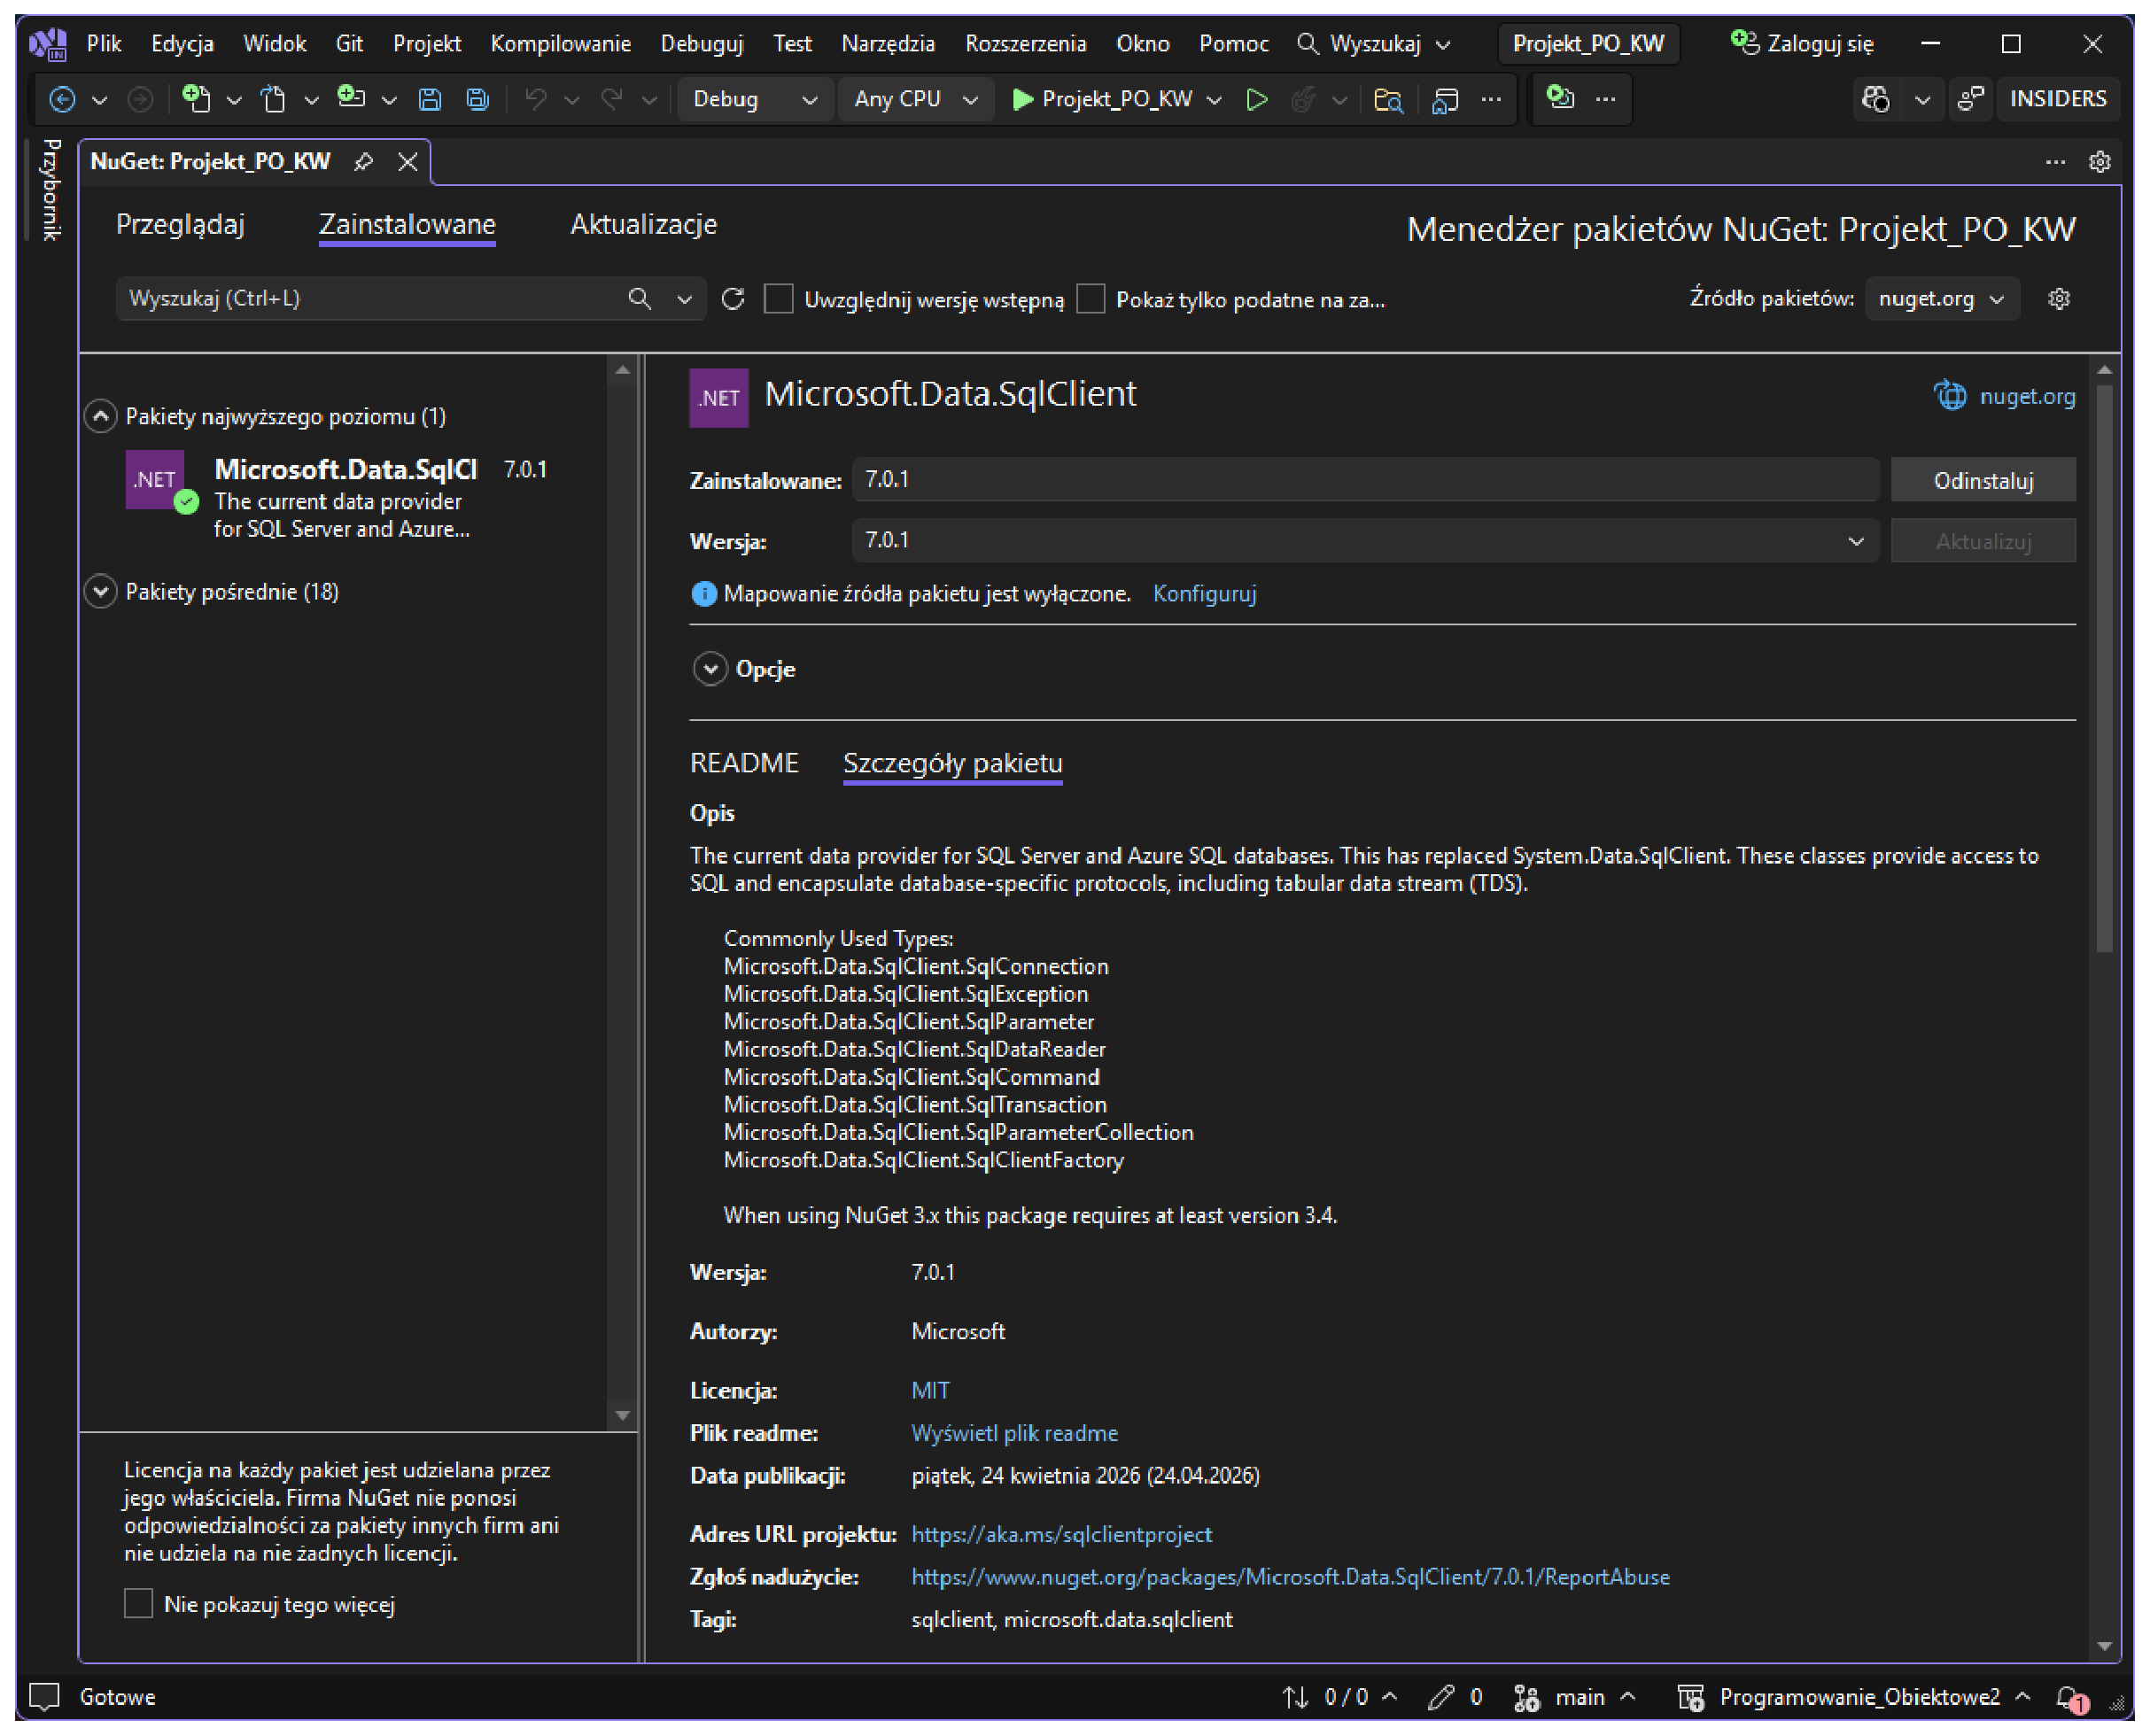
\includegraphics[width=\linewidth]{figures/fig_001.eps}
\caption{Sterownik Microsoft.Data.SqlClient (Menadżer pakietów NuGet).\label{fig1}}
\end{figure}

Baza danych składa się z ośmiu tabel: 
Uzytkownik, Pupil, Weterynarz, Zabieg, 
Rezerwacja, Dostepnosc oraz tabel łączących 
Uzytkownik\_Pupil i Weterynarz\_Zabieg. 
Tabela Uzytkownik oraz Pupil połączone są relacją 
wiele do wielu za pomocą tabeli łączącej Uzytkownik\_Pupil, 
tzn. jeden użytkownik może posiadać wiele pupili i jeden pupil może 
mieć wielu właścicieli. Tabela Weterynarz oraz Zabieg
połączone są relacją wiele do wielu za pomocą tabeli 
Weterynarz\_Zabieg, co oznacza, że jeden weterynarz może 
wykonywać wiele zabiegów, a jeden zabieg może być wykonywany przez 
wielu weterynarzy. Tabela Dostepnosc powiązana jest z tabelą 
Weterynarz relacją jeden do wielu i przechowuje informacje 
o godzinach pracy weterynarza w poszczególnych dniach tygodnia. 
Tabela Rezerwacja stanowi centralną tabelę systemu i łączy 
w sobie informacje o użytkowniku, pupilu, weterynarzu oraz zabiegu, 
przechowując datę, godzinę oraz aktualny status wizyty.

\begin{table}[H]
\centering
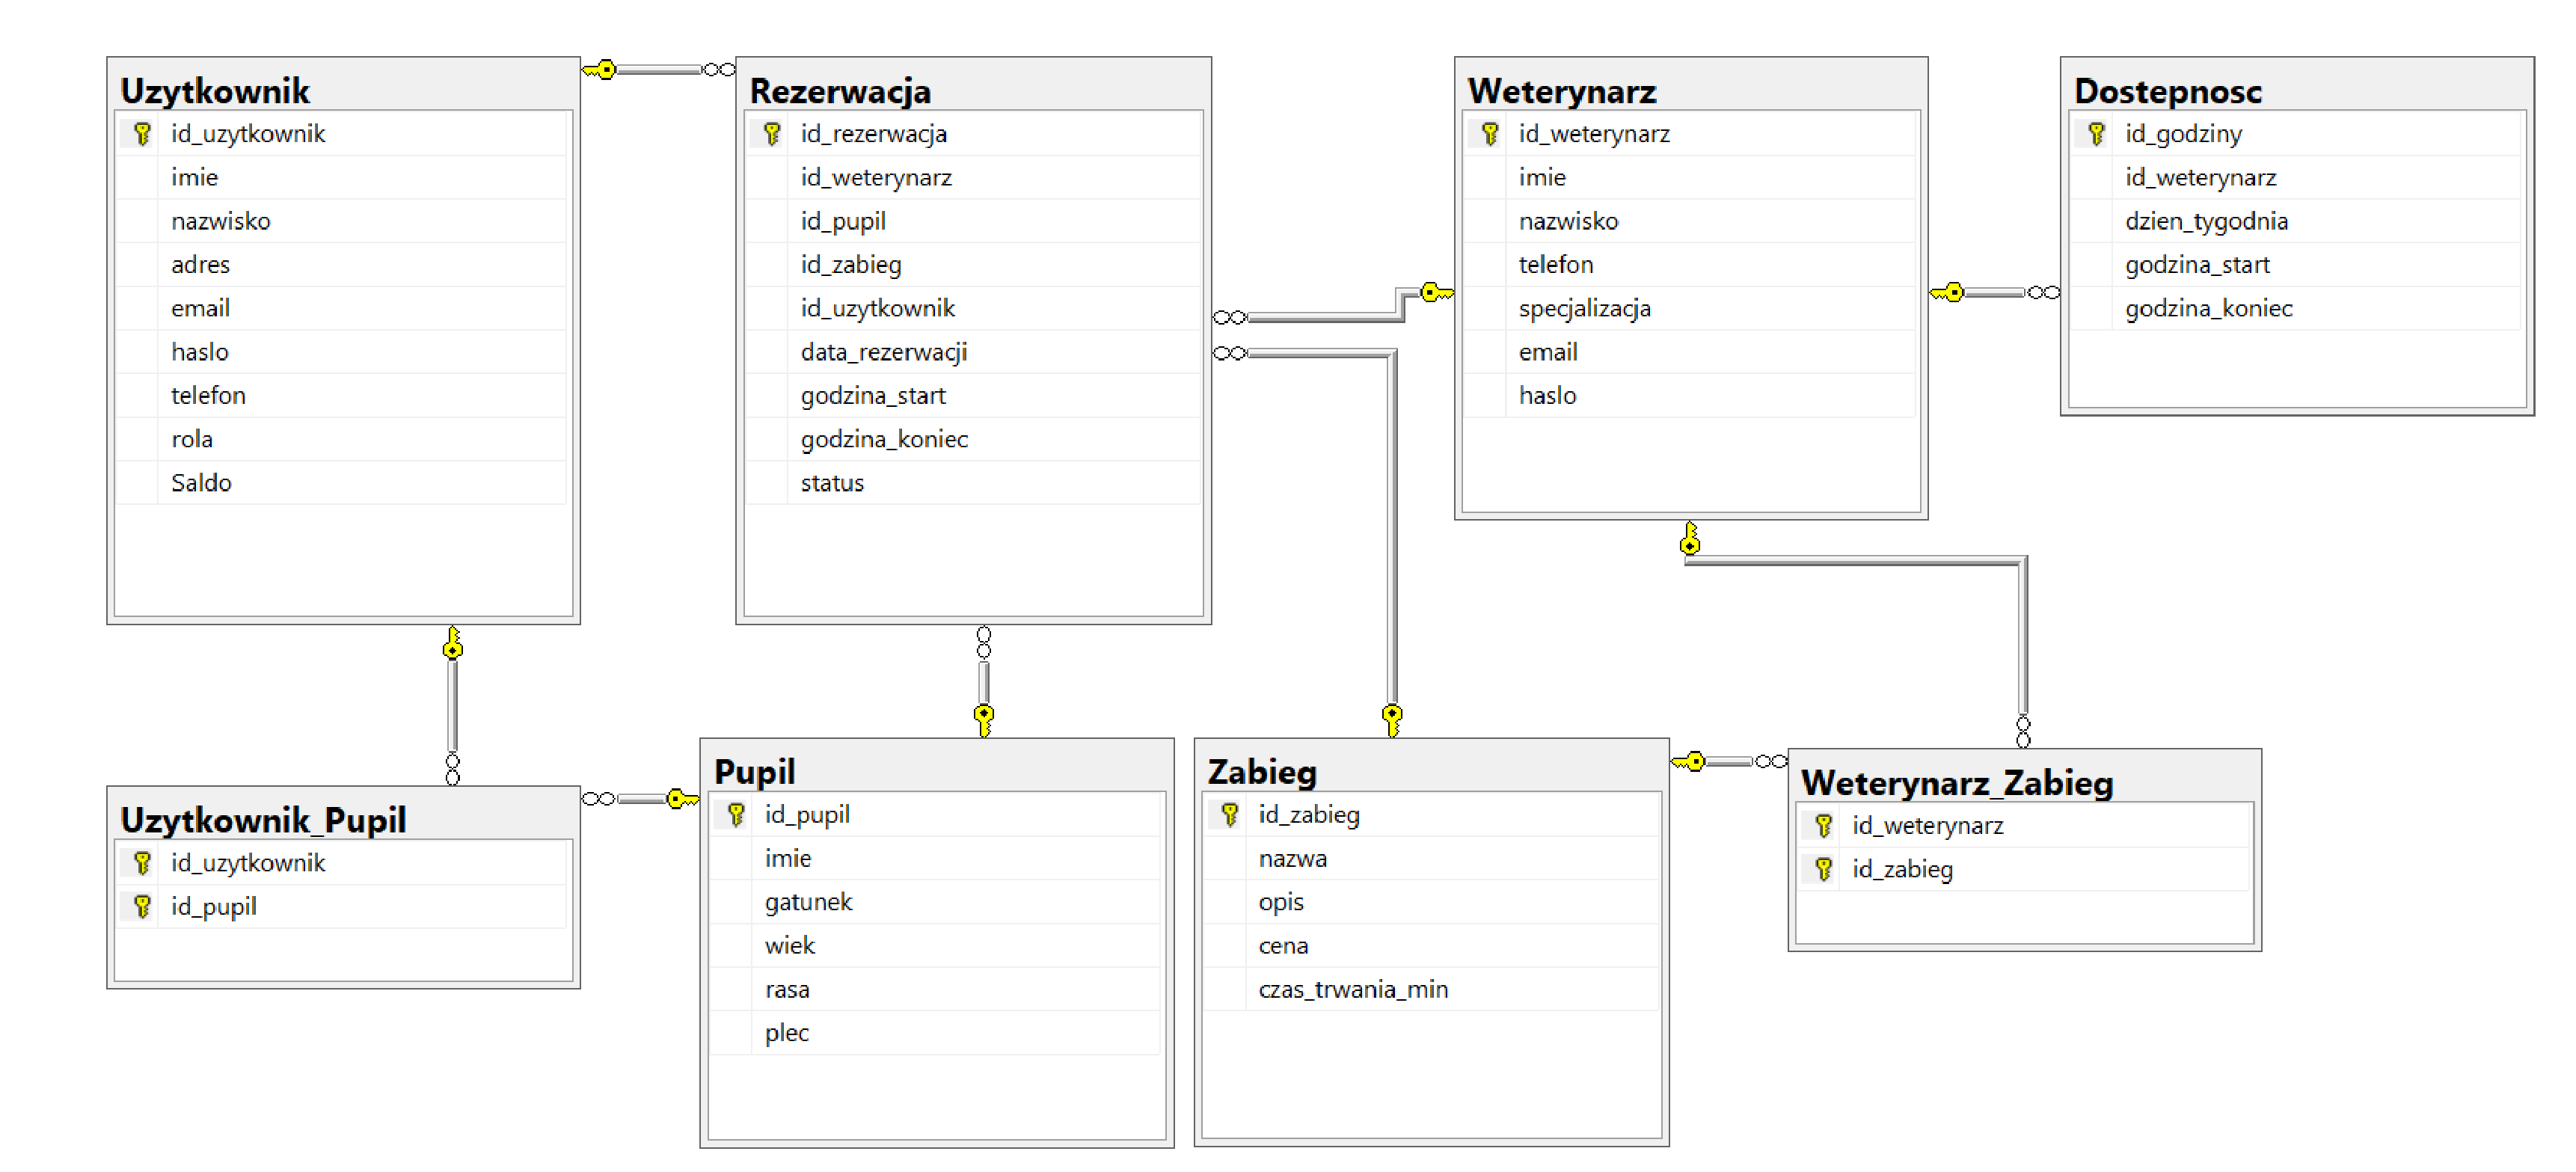
\includegraphics[width=1.15\linewidth]{figures/fig_002.eps}
\caption{Diagram ERD projektowanej aplikacji.\label{fig2}}
\end{table}

\subsection{Normalizacja bazy oraz Integralność danych}

\textbf{Normalizacja bazy danych}

Baza danych została zaprojektowana zgodnie z trzecią postacią normalną (3NF). 
Każda tabela zawiera tylko atrybuty bezpośrednio zależne od klucza głównego, eliminując redundancję 
danych. Relacje wiele do wielu (Uzytkownik-Pupil oraz WeterynarzZabieg) zostały 
rozwiązane przy użyciu dedykowanych tabel łączących.

\textbf{Integralność danych}

Integralność danych w bazie zapewniana jest przez następujące mechanizmy:
\begin{itemize}
\item \textbf{Klucze główne} - każda tabela posiada unikalny identyfikator typu INT IDENTITY, automatycznie 
inkrementowany przez SQL Server,
\item \textbf{Klucze obce} - relacje między tabelami są wymuszane przez ograniczenia FOREIGN KEY, uniemożliwiające 
dodanie rekordów z nieistniejącymi odwołaniami,
\item \textbf{Ograniczenia CHECK} - kolumny gatunek (Pies/Kot), plec (Samiec/Samica), rola (Uzytkownik/Administrator)
oraz status (Zarezerwowany/Anulowany/Zrealizowany) posiadają ograniczenia dopuszczalnych wartości,
\item \textbf{Unikalność} - kolumna email w tabeli Uzytkownik posiada ograniczenie UNIQUE, uniemożliwiające 
rejestrację dwóch kont na ten sam adres e-mail,
\item \textbf{Walidacja po stronie aplikacji} - dodatkowa weryfikacja danych wejściowych realizowana jest w
kodzie C\# przed wykonaniem zapytań do bazy danych, co stanowi drugą warstwę ochrony przed nieprawidłowymi danymi.
\end{itemize}

\section{Struktura klas}

Projekt podzielony jest na cztery warstwy: Models (klasy odwzorowujące tabele bazy danych), 
Repositories (klasy odpowiedzialne za komunikację z bazą danych 
poprzez ADO.NET), Views (okna WPF) oraz 
Helpers (klasy pomocnicze tzn. SessionHelper i DialogHelper). 
Klasa Database odpowiada za nawiązanie 
połączenia z bazą danych SQL Server.

\begin{figure}[H]
\centering
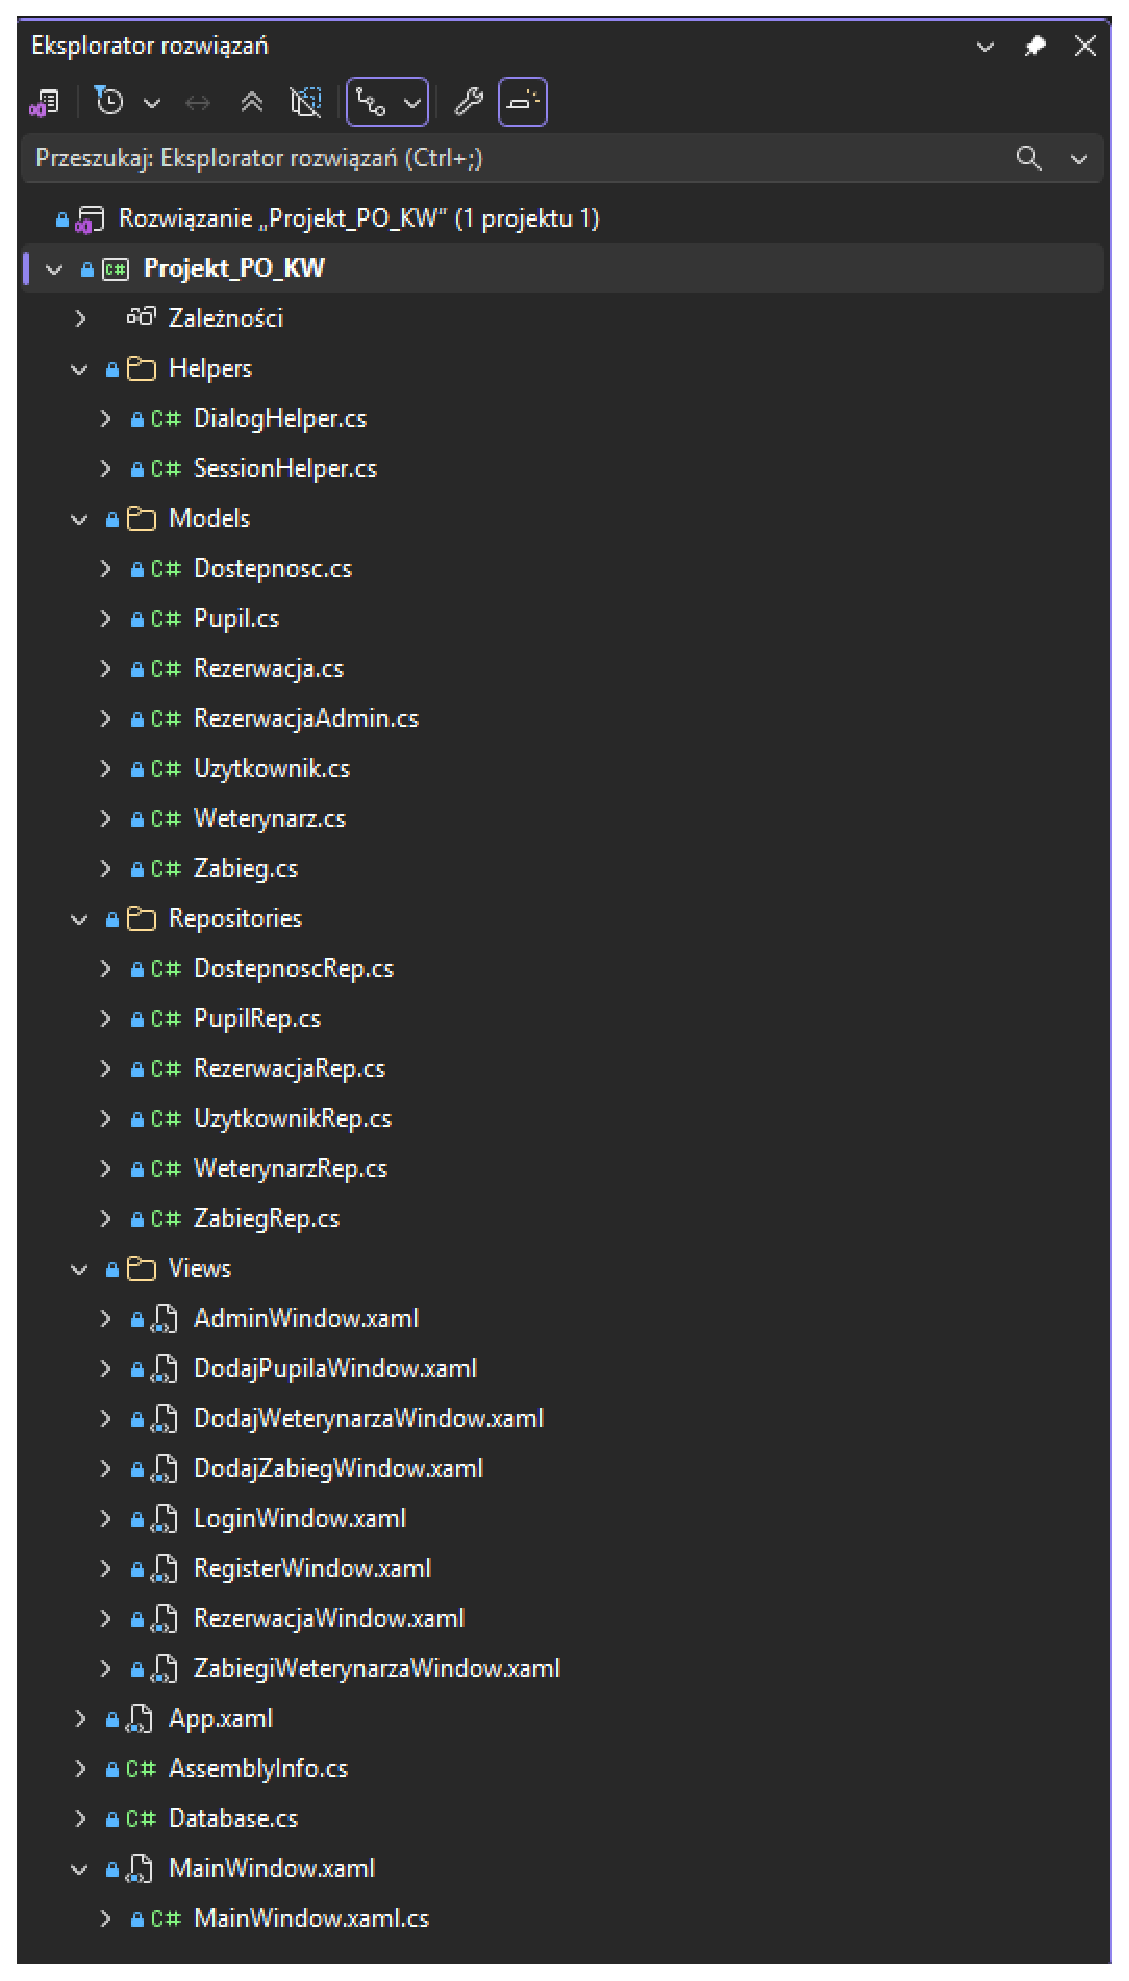
\includegraphics[width=0.9\linewidth]{figures/fig_003.eps}
\caption{Struktura klas w projekcie.\label{fig3}}
\end{figure}

\section{Najważniejsze metody}

\subsection{Logowanie}

Metoda Zaloguj\_sie pobiera wartości z pól formularza: adres e-mail oraz hasło. 
Następnie sprawdza, czy oba pola zostały uzupełnione, jeśli nie to wyświetlany jest komunikat błędu. Jeżeli pola są wypełnione, wywoływana 
jest metoda GetUser z repozytorium UzytkownikRep, która wykonuje zapytanie SQL do bazy danych i zwraca obiekt użytkownika 
na podstawie podanego adresu e-mail oraz hasła. Jeśli użytkownik nie zostanie znaleziony w bazie danych, wyświetlany jest komunikat o 
nieprawidłowych danych logowania. W przypadku pomyślnego uwierzytelnienia dane zalogowanego użytkownika zapisywane są w klasie
SessionHelper, która przechowuje je przez cały czas działania aplikacji. Następnie sprawdzana jest rola przypisana do konta, jeśli jest 
to administrator, otwierany jest panel administratora AdminWindow, w przeciwnym razie otwierany jest panel użytkownika w tym wypadku MainWindow. 
Okno logowania zostaje zamknięte. W przypadku błędu połączenia z bazą danych wyświetlany jest komunikat z informacją o przyczynie błędu.

\lstinputlisting[caption=Metoda logowania wraz z SessionHelper oraz metodą z zapytaniem SQL, label=logowanie]{src/Task1.cs}

\subsection{Zmiana hasła - panel użytkownika}

Metoda Zmiana\_hasla pobiera dane zalogowanego użytkownika z klasy SessionHelper. 
Następnie odczytuje wartości z trzech pól formularza tzn. obecne hasło, nowe hasło oraz potwierdzenie hasła. 
Sprawdza, czy wszystkie pola zostały uzupełnione jeśli nie, wyświetlany jest komunikat błędu. Następnie weryfikuje, 
czy podane obecne hasło zgadza się z hasłem przechowywanym w sesji jeśli nie, wyświetlany jest komunikat o nieprawidłowym haśle.
Kolejnym krokiem jest sprawdzenie, czy nowe hasło jest identyczne z polem potwierdzającym oraz czy jego długość wynosi co najmniej 6 znaków.
Przed wykonaniem zmiany użytkownik proszony jest o potwierdzenie operacji w oknie dialogowym. Następnie wywoływana jest metoda Zmiana\_hasla 
z repozytorium UzytkownikRep, która wykonuje 
zapytanie UPDATE aktualizujące hasło w bazie danych na podstawie identyfikatora użytkownika. Po pomyślnym wykonaniu operacji pola formularza zostają 
wyczyszczone, a użytkownik otrzymuje komunikat o sukcesie. W przypadku błędu połączenia z bazą danych wyświetlany 
jest komunikat z informacją o przyczynie błędu.

\lstinputlisting[caption=Metoda zmiany hasła wraz z metodą zapytania SQL, label=zmiana hasla]{src/Task2.cs}

\subsection{Zmiana panelu wyświetlania - panel użytkownika}

Metoda Nav\_Click odpowiada za nawigację między sekcjami panelu użytkownika. Na początku wszystkie 
panele tzn. PanelMojeKonto, PanelMojePupile, PanelMojeWizyty oraz PanelDoladujSrodki są ukrywane poprzez 
ustawienie właściwości Visibility na Collapsed, a znaczniki aktywności wszystkich przycisków nawigacyjnych są zerowane. 
Następnie kliknięty przycisk zostaje oznaczony jako aktywny poprzez ustawienie jego właściwości Tag na wartość active. W zależności od 
tego, który przycisk został kliknięty, wyświetlany jest odpowiedni panel. 
W przypadku sekcji Moje pupile dodatkowo wywoływana jest metoda WczytajPupile, która pobiera listę pupili zalogowanego 
użytkownika z bazy danych. Analogicznie w przypadku sekcji Moje wizyty wywoływana jest metoda WczytajWizyty, która pobiera 
historię rezerwacji użytkownika.

\lstinputlisting[caption=Metoda nawigacji do zmiany panelu wyświetlania, label=zmiana panelu wyświetlania]{src/Task3.cs}

\subsection{Wpłata środków - panel użytkownika}

Metoda WplacSrodki\_Click umożliwia użytkownikowi doładowanie salda konta. Pobiera wartość wpisaną przez użytkownika 
w polu tekstowym i próbuje przekonwertować ją na liczbę całkowitą przy użyciu metody int.TryParse. 
Jeśli podana wartość nie jest liczbą całkowitą lub jest mniejsza bądź równa zero, wyświetlany jest komunikat błędu. W przypadku 
poprawnych danych użytkownik proszony jest o potwierdzenie operacji w oknie dialogowym. Po zatwierdzeniu wywoływana jest 
metoda DoladujSaldo z repozytorium UzytkownikRep, która wykonuje zapytanie UPDATE zwiększające saldo 
użytkownika w bazie danych o podaną kwotę. Jednocześnie saldo aktualizowane jest w obiekcie przechowywanym w SessionHelper 
oraz odświeżana jest etykieta wyświetlająca aktualne saldo w interfejsie użytkownika. Pole tekstowe zostaje wyczyszczone, a użytkownik 
otrzymuje komunikat o pomyślnym wykonaniu wpłaty. W przypadku błędu połączenia z bazą danych wyświetlany jest 
komunikat z informacją o przyczynie błędu.

\lstinputlisting[caption=Metoda wpłaty środków wraz z metodą zapytania SQL, label=wpłata środków]{src/Task4.cs}

\subsection{Rezerwacja zabiegu - panel użytkownika}

Metoda WybierzZabieg obsługuje wybór zabiegu przez użytkownika w pierwszym kroku rezerwacji. 
Na początku iteruje po wszystkich elementach listy zabiegów i resetuje kolor obramowania każdego z nich do 
domyślnego koloru szarego, aby usunąć poprzednie zaznaczenie. Następnie pobiera kliknięty element jako obiekt Border i zmienia 
kolor jego obramowania na różowy, sygnalizując aktywny wybór. Wybrany zabieg zostaje zapisany w polu \_wybranyZabieg
jako obiekt typu Zabieg, pobierany z kontekstu danych klikniętego elementu.

\lstinputlisting[caption=Metoda wyboru zabiegu oraz wyboru weterynarza, label=Rezerwacja zabiegu (1-3)]{src/Task5.cs}

Metoda Dalej\_Click obsługuje nawigację między trzema krokami procesu rezerwacji wizyty. W pierwszym kroku sprawdza, czy 
użytkownik wybrał pupila z listy rozwijanej oraz czy zaznaczył zabieg jeśli nie, wyświetlany jest odpowiedni komunikat błędu. 
Następnie weryfikuje, czy saldo konta użytkownika jest wystarczające do pokrycia kosztu wybranego zabiegu. Jeśli środki są niewystarczające,
wyświetlany jest komunikat informujący o aktualnym saldzie oraz koszcie zabiegu. W przypadku poprawnej walidacji pobierana jest lista weterynarzy 
wykonujących wybrany zabieg przy użyciu metody GetByZabieg z repozytorium WeterynarzRep, która wykonuje zapytanie SELECT z 
połączeniem tabel Weterynarz i Weterynarz\_Zabieg. W drugim kroku sprawdzane jest, czy 
użytkownik wybrał weterynarza jeśli tak, wywoływana jest metoda WygenerujKalendarz i interfejs przełącza się na trzeci krok, a przycisk Dalej
zmienia treść na Zarezerwuj. W trzecim a zarazem ostatnimkroku sprawdzane jest, czy użytkownik wybrał termin jeśli tak, wywoływana jest metoda ZapiszRezerwacje.

\lstinputlisting[caption=Metoda do rezerwacji (zachowania ciągłąści między etapami) wraz z metodą zapytania SQL, label=Rezerwacja zabiegu (2-3)]{src/Task6.cs}

Metoda WygenerujKalendarz odpowiada za dynamiczne generowanie tygodniowego widoku kalendarza dostępności wybranego 
weterynarza. Na początku czyszczone są wszystkie elementy siatki kalendarza. Następnie pobierana jest dostępność weterynarza z 
bazy danych przy użyciu metody GetByWeterynarz z repozytorium DostepnoscRep, która wykonuje 
zapytanie SELECT zwracające godziny pracy weterynarza w poszczególnych dniach tygodnia. Na podstawie pobranych danych 
generowana jest lista dni tygodnia od dnia dzisiejszego, dla których weterynarz ma zdefiniowane godziny pracy. Dla każdego dnia dodawana 
jest kolumna do siatki kalendarza z nagłówkiem zawierającym nazwę dnia i datę. Następnie pobierane są istniejące rezerwacje weterynarza z 
bazy danych. Dla każdej godziny od 8:00 do 16:00 oraz dla każdego dostępnego dnia generowany jest przycisk, którego stan zależy od trzech 
warunków: czy dany slot mieści się w godzinach pracy weterynarza, czy godzina zakończenia zabiegu nie przekracza końca jego pracy oraz czy 
w danym terminie nie istnieje już inna rezerwacja. Przyciski oznaczone są kolorami tzn. zielonym dla wolnych terminów, czerwonym dla zajętych 
oraz szarym dla terminów poza godzinami pracy. Po kliknięciu wolnego slotu poprzednio wybrany termin zostaje zresetowany, a nowo wybrany 
zostaje podświetlony na różowo z etykietą Wybrano. Wybrana data i godzina zapisywane są w odpowiednich polach.

\lstinputlisting[caption=Metoda wyświetląjąca kalendarz wraz z metodą zapytania SQL, label=Rezerwacja zabiegu (3-3)]{src/Task7.cs}

\subsection{Lista użytkowników - panel administratora}

Metoda WczytajUzytkownikow pobiera listę wszystkich zarejestrowanych użytkowników z bazy danych przy użyciu metody 
GetAllUzytkownicy z repozytorium UzytkownikRep i przypisuje ją jako źródło danych do listy użytkowników 
w interfejsie. Metoda GetAllUzytkownicy wykonuje zapytanie SELECT pobierające wszystkich użytkowników z 
rolą Uzytkownik, posortowanych według nazwiska.

Metoda UsunUzytkownika\_Click obsługuje usunięcie użytkownika przez administratora. 
Pobiera identyfikator użytkownika z właściwości Tag klikniętego przycisku i wyświetla okno 
dialogowe z prośbą o potwierdzenie operacji, informując że usunięcie użytkownika spowoduje również usunięcie 
jego pupili i rezerwacji. Po potwierdzeniu wywoływana jest metoda UsunUzytkownika z 
repozytorium UzytkownikRep i lista użytkowników jest odświeżana. Metoda UsunUzytkownika
wykonuje operację usunięcia w kilku krokach: najpierw usuwa wszystkie rezerwacje użytkownika, następnie pobiera listę 
jego pupili, usuwa powiązania użytkownika z pupilami z tabeli Uzytkownik\_Pupil, a następnie 
dla każdego pupila sprawdza, czy nie posiada już innych właścicieli jeśli nie, pupil zostaje trwale usunięty z tabeli 
Pupil. Na końcu usuwany jest sam rekord użytkownika z tabeli Uzytkownik.

\lstinputlisting[caption=Metody usuwania i wczytywania użytkowników wraz z metodą zapytania SQL, label=lista użytkowników]{src/Task8.cs}

\subsection{Dodawanie weterynarza - panel administratora}

Metoda DodajWeterynarza\_Click obsługuje dodawanie nowego weterynarza przez administratora. Pobiera wartości ze wszystkich 
pól formularza i sprawdza, czy wymagane pola (imię, nazwisko, email oraz hasło) zostały uzupełnione jeśli nie, wyświetlany jest 
komunikat błędu. W przypadku poprawnej walidacji wywoływana jest metoda Dodaj z repozytorium WeterynarzRep, 
która wykonuje zapytanie INSERT dodające nowego weterynarza do tabeli Weterynarz w bazie danych. Następnie 
pobierany jest identyfikator nowo dodanego weterynarza przy użyciu metody GetIdByEmail. Dla każdego dnia tygodnia od 
poniedziałku do piątku wywoływana jest metoda pomocnicza ZapiszDostepnosc, która sprawdza, czy pola godzin zostały 
uzupełnione oraz czy godzina rozpoczęcia jest wcześniejsza niż godzina zakończenia jeśli warunki są spełnione, wywoływana 
jest metoda Dodaj z repozytorium DostepnoscRep, która wykonuje zapytanie INSERT zapisujące godziny 
pracy weterynarza w danym dniu tygodnia do tabeli Dostepnosc. Jeśli pola godzin dla danego dnia są puste, wpis dla 
tego dnia nie jest tworzony, co oznacza że weterynarz nie pracuje w tym dniu.

\lstinputlisting[caption=Metoda dodawania weterynarza wraz z metodami zapytań SQL, label=dodawanie weterynarza]{src/Task9.cs}

\subsection{Dodawanie zabiegu - panel administratora}

Metoda Dodaj\_Click w oknie DodajZabiegWindow obsługuje dodawanie 
nowego zabiegu przez administratora. Pobiera wartości z trzech pól formularza: nazwę zabiegu, czas trwania oraz cenę. 
Sprawdza, czy wszystkie pola zostały uzupełnione jeśli nie, wyświetlany jest komunikat błędu. Następnie weryfikuje, 
czy podany czas trwania jest poprawną dodatnią liczbą całkowitą przy użyciu metody int.TryParse, oraz czy cena 
jest poprawną nieujemną liczbą dziesiętną przy użyciu metody decimal.TryParse. W przypadku poprawnej walidacji 
wywoływana jest metoda Dodaj z repozytorium ZabiegRep, która wykonuje zapytanie INSERT dodające nowy 
zabieg do tabeli Zabieg w bazie danych. Pole opis jest opcjonalne jeśli nie zostało uzupełnione, do bazy zapisywana 
jest wartość NULL. 

Natomiast metoda UsunZabieg\_Click obsługuje usunięcie zabiegu. Pobiera identyfikator zabiegu z właściwości Tag
klikniętego przycisku i wyświetla okno dialogowe z prośbą o potwierdzenie operacji, informując że usunięcie zabiegu spowoduje również usunięcie 
powiązanych rezerwacji. Po potwierdzeniu wywoływana jest metoda Usun z repozytorium ZabiegRep, która wykonuje operację usunięcia 
w trzech krokach: najpierw usuwa wszystkie rezerwacje powiązane z danym zabiegiem z tabeli Rezerwacja, następnie usuwa powiązania z 
weterynarzami z tabeli Weterynarz\_Zabieg, a na końcu usuwa sam rekord zabiegu z tabeli Zabieg. 
Po pomyślnym usunięciu lista zabiegów jest odświeżana.

\lstinputlisting[caption=Metody dodawania i usuwania zabiegów wraz z metodami zapytań SQL, label=dodawanie zabiegu]{src/Task10.cs}

\subsection{Operacje na zabiegach - panel administratora}

Metoda WczytajRezerwacje pobiera wszystkie rezerwacje z bazy danych przy użyciu metody GetAllAdmin z repozytorium RezerwacjaRep, 
która wykonuje zapytanie SELECT z czterokrotnym połączeniem tabel Weterynarz, Pupil, Zabieg, Uzytkownik w 
celu pobrania pełnych informacji o każdej rezerwacji, takich jak imię i nazwisko weterynarza, imię pupila, nazwa zabiegu oraz imię i nazwisko właściciela.
Wyniki są sortowane malejąco według daty rezerwacji. Pobrana lista zapisywana jest w polu \_wszystkieRezerwacje, a 
następnie wywoływana jest metoda ZastosujFiltry.

Metoda ZastosujFiltry filtruje listę wszystkich rezerwacji na podstawie trzech kryteriów: wybranej daty, wybranego weterynarza oraz wybranego statusu. 
Filtrowanie odbywa się sekwencyjnie tzn. każdy aktywny filtr zawęża zbiór wyników. Aby uniknąć wywoływania filtrowania podczas inicjalizacji kontrolek, metoda 
sprawdza flagę \_inicjalizacja. Metoda WyczyscFiltry\_Click resetuje wszystkie filtry do wartości domyślnych i ponownie wywołuje ZastosujFiltry.

Metoda StatusRezerwacji\_Changed obsługuje zmianę statusu rezerwacji bezpośrednio z poziomu listy. 
Pobiera identyfikator rezerwacji z właściwości Tag listy rozwijanej oraz nową wartość statusu z wybranego elementu. 
Następnie wywołuje metodę ZmienStatus z repozytorium RezerwacjaRep, która wykonuje zapytanie UPDATE
aktualizujące status rezerwacji w bazie danych.

Metoda AktualizujPrzeterminowane wywoływana jest automatycznie przy każdym uruchomieniu aplikacji w klasie App.xaml.cs. 
Wykonuje zapytanie UPDATE zmieniające status wszystkich rezerwacji o statusie Zarezerwowany, których godzina 
zakończenia już minęła, na status Zrealizowany. Dzięki temu system automatycznie aktualizuje historię wizyt.

\lstinputlisting[caption=Metoda aktualizacji statusów oraz metody związane z zabiegami wraz z metodami zapytań SQL, label=lista zabiegów]{src/Task11.cs}

\section{Wymagania sprzętowe i narzędzia}

\begin{itemize}
\item \textbf{Procesor:} minimum 2-rdzeniowy, 2.0 GHz lub szybszy.
\item \textbf{Pamięć RAM:} minimum 8 GB.
\item \textbf{System operacyjny:} Windows 10 (64-bit) lub nowszy.
\item \textbf{.NET:} wersja 10.0 lub nowsza.
\item \textbf{Microsoft SQL Server:} wersja 2025 (wersja używana w projekcie).
\item \textbf{Visual Studio Insiders:} wersja 2026 (wersja używana w projekcie).
\item \textbf{Sterownik ADO.NET:} Microsoft.Data.SqlClient w wersji 7.0.1 
(instalowany przez NuGet).
\end{itemize}

\textbf{Narzędzia wykorzystane w projekcie}

\begin{itemize}
\item \textbf{Visual Studio Insiders 2026} - środowisko programistyczne do tworzenia aplikacji w języku C\#,
\item \textbf{Git} - system kontroli wersji,
\item \textbf{WPF (Windows Presentation Foundation)} - technologia do tworzenia graficznego interfejsu użytkownika,
\item \textbf{Microsoft SQL Server 2025} - system zarządzania relacyjną bazą danych,
\item \textbf{SQL Server Management Studio (SSMS)} - narzędzie do zarządzania bazą danych SQL Server,
\item \textbf{Microsoft.Data.SqlClient 7.0.1} - sterownik ADO.NET do komunikacji z bazą danych SQL Server,
\item \textbf{Strona online-convert.com} - strona wykorzystana do konwersji grafik do formatu EPS.
\end{itemize}
\chapter{Harmonogram realizacji projektu}

W realizacji projektu użyłem Git jako systemu kontroli wersji, a repozytorium jest zapisane na platformie GitHub 
pod adresem: \url{https://github.com/lukaszwarzocha/Programowanie_Obiektowe2.git}.

\vspace{10pt}

Realizację projektu przedstawiam na diagramie Gantta. Prace rozpocząłem od przygotowania projektu, które obejmowało m.in. 
zaprojektowanie bazy danych, stworzenie modeli oraz konfigurację połączenia z bazą danych. 
Następnie przystąpiłem do tworzenia interfejsu graficznego w technologii WPF równolegle tworząc implementację panelu użytkownika. 
Kolejnym etapem była implementacja panelu administratora. Ostatnim etapem było tworzenie dokumentacji do projektu.

\begin{figure}[H]
\centering

\includegraphics[width=\linewidth]{figures/fig_004.eps}
\caption{Diagram Gantta.\label{fig4}}
\end{figure}
\chapter{Prezentacja warstwy użytkowej projektu}

\section{Panel logowania oraz rejestracji}

Panel logowania umożliwia użytkownikowi 
uwierzytelnienie się w systemie. Formularz zawiera dwa pola: adres e-mail oraz hasło. Po 
kliknięciu przycisku Zaloguj się aplikacja weryfikuje poprawność wprowadzonych danych. Po poprawnym 
zalogowaniu użytkownik zostaje przekierowany do panelu użytkownika lub panelu administratora, w z
ależności od przypisanej roli. Użytkownik nieposiadający konta może przejść do formularza rejestracji klikając przycisk Zarejestruj się.

\begin{figure}[H]
\centering
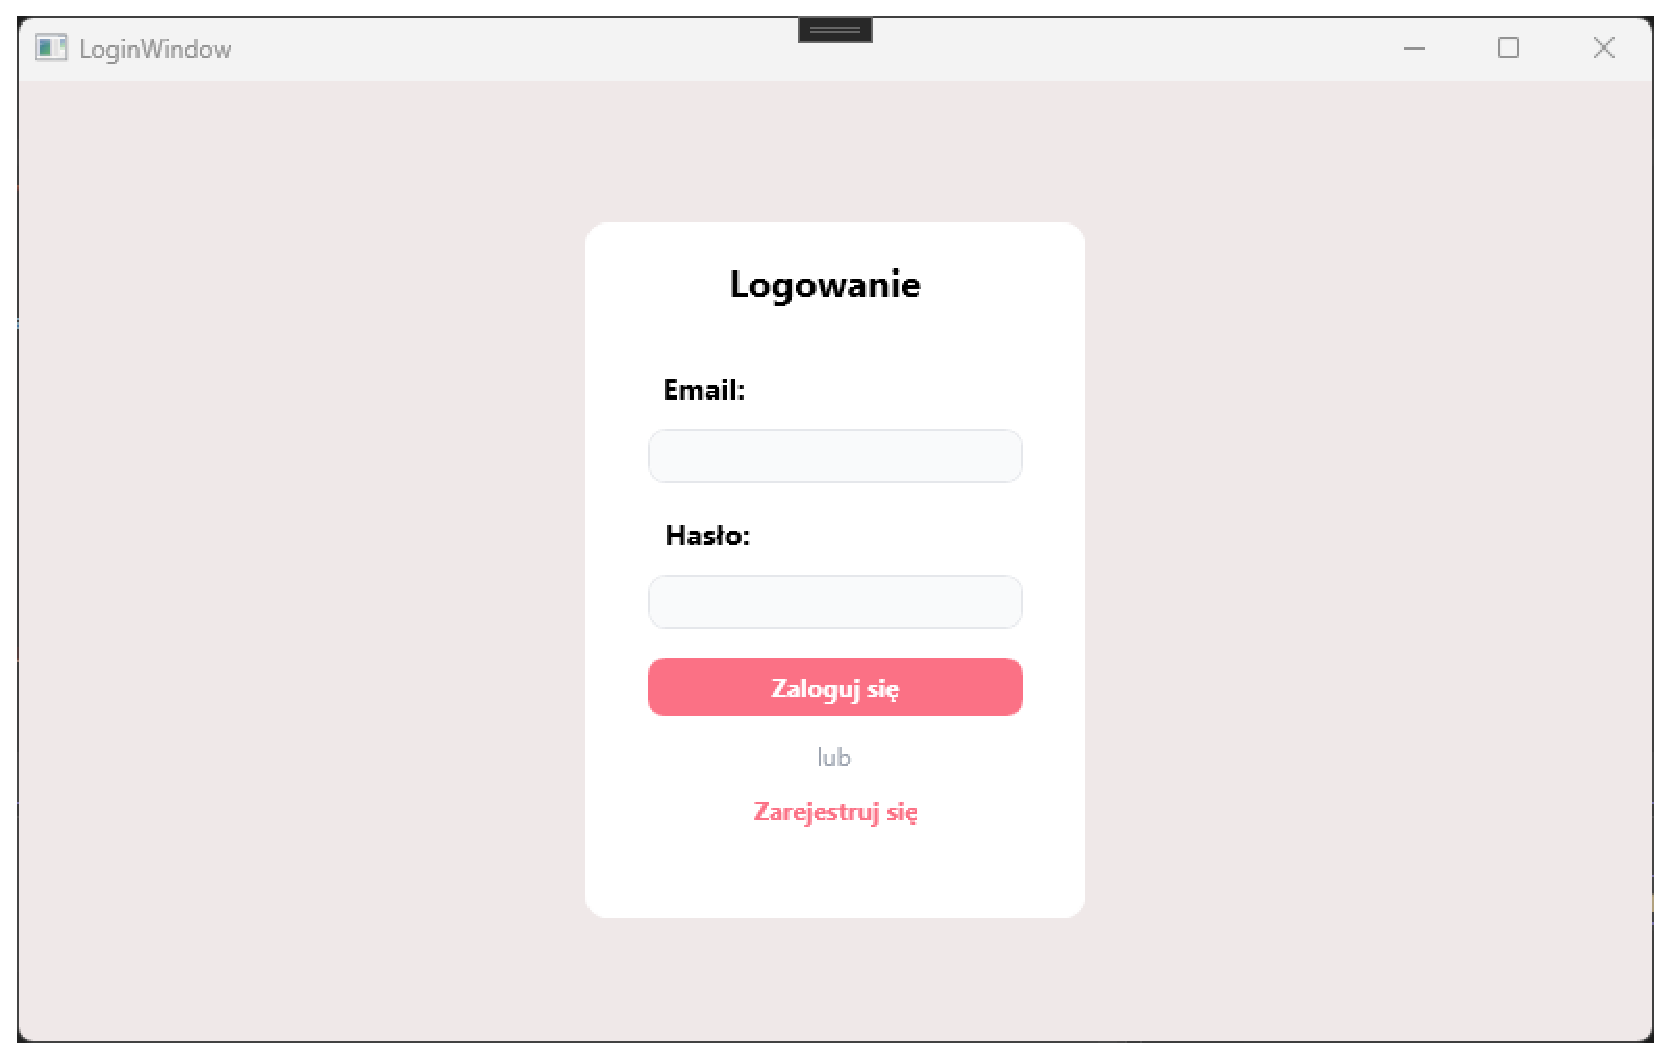
\includegraphics[width=0.8\linewidth]{figures/Logowanie/fig_005.eps}
\caption{Widok panelu logowania.\label{fig5}}
\end{figure}

W przypadku gdy użytkownik nie wypełni pól formularza lub poda błędne dane logowania, wyświetlany jest 
komunikat błędu informujący o nieprawidłowym adresie e-mail lub haśle.

\begin{figure}[H]
\centering
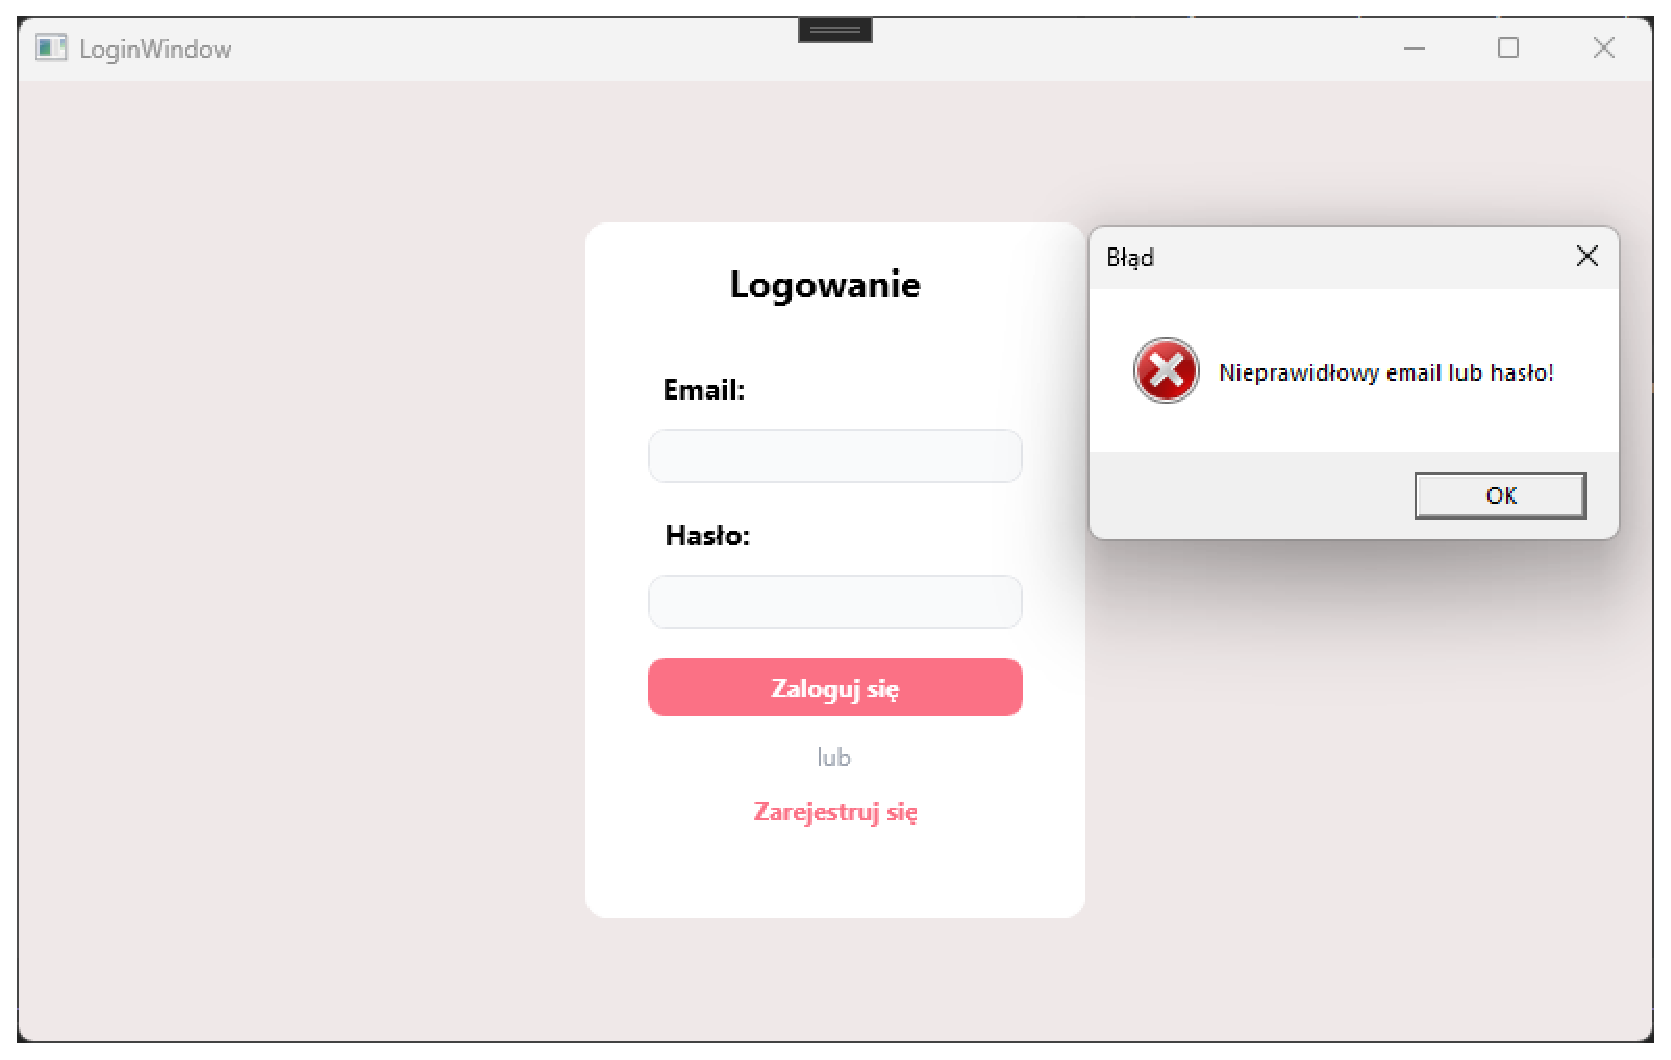
\includegraphics[width=0.8\linewidth]{figures/Logowanie/fig_006.eps}
\caption{Komunikat błędu przy nieprawidłowych danych logowania.\label{fig6}}
\end{figure}

\textbf{Panel rejestracji}

Panel rejestracji umożliwia nowemu użytkownikowi założenie konta w systemie. Formularz zawiera pola: imię, 
nazwisko, adres e-mail, numer telefonu, adres (pole opcjonalne), hasło oraz potwierdzenie hasła. 
Po wypełnieniu formularza i kliknięciu przycisku Zarejestruj się aplikacja przeprowadza 
wieloetapową walidację danych. Użytkownik posiadający już konto może powrócić do ekranu logowania klikając przycisk Powróć do logowania.

\begin{figure}[H]
\centering
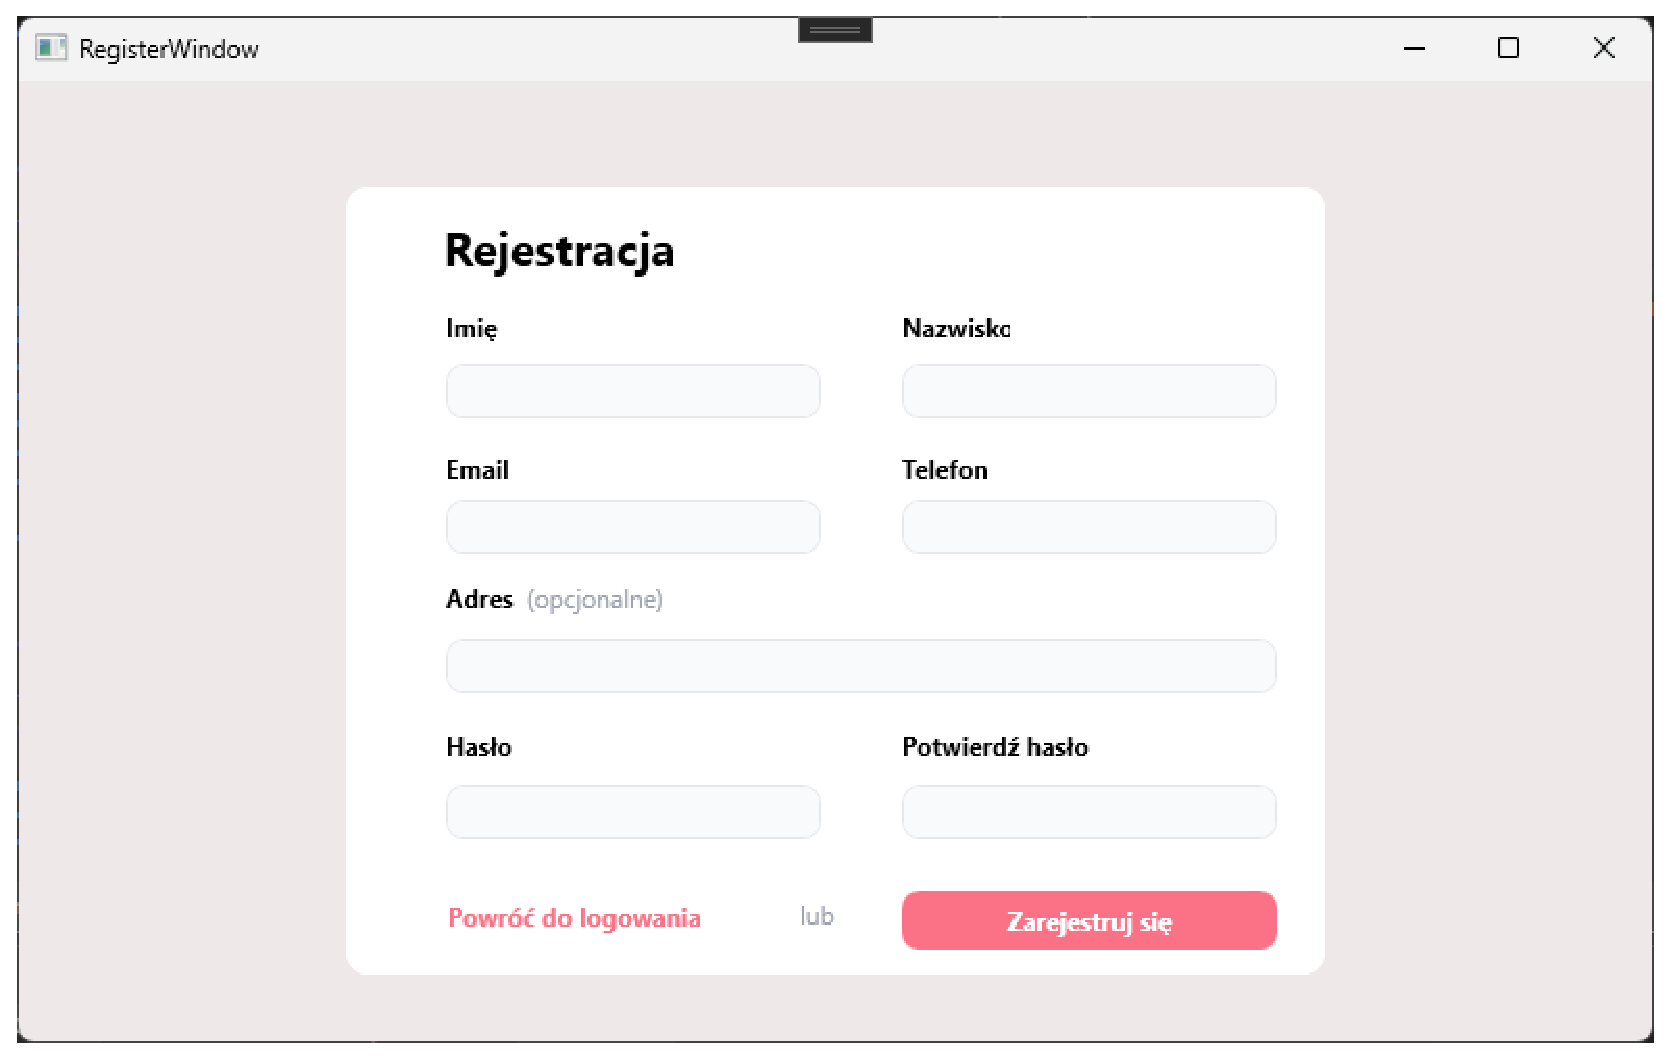
\includegraphics[width=0.8\linewidth]{figures/Rejestracja/fig_007.eps}
\caption{Widok panelu rejestracji.\label{fig7}}
\end{figure}

W przypadku gdy użytkownik nie wypełni wszystkich wymaganych pól formularza, wyświetlany jest komunikat błędu informujący o konieczności uzupełnienia danych.

\begin{figure}[H]
\centering
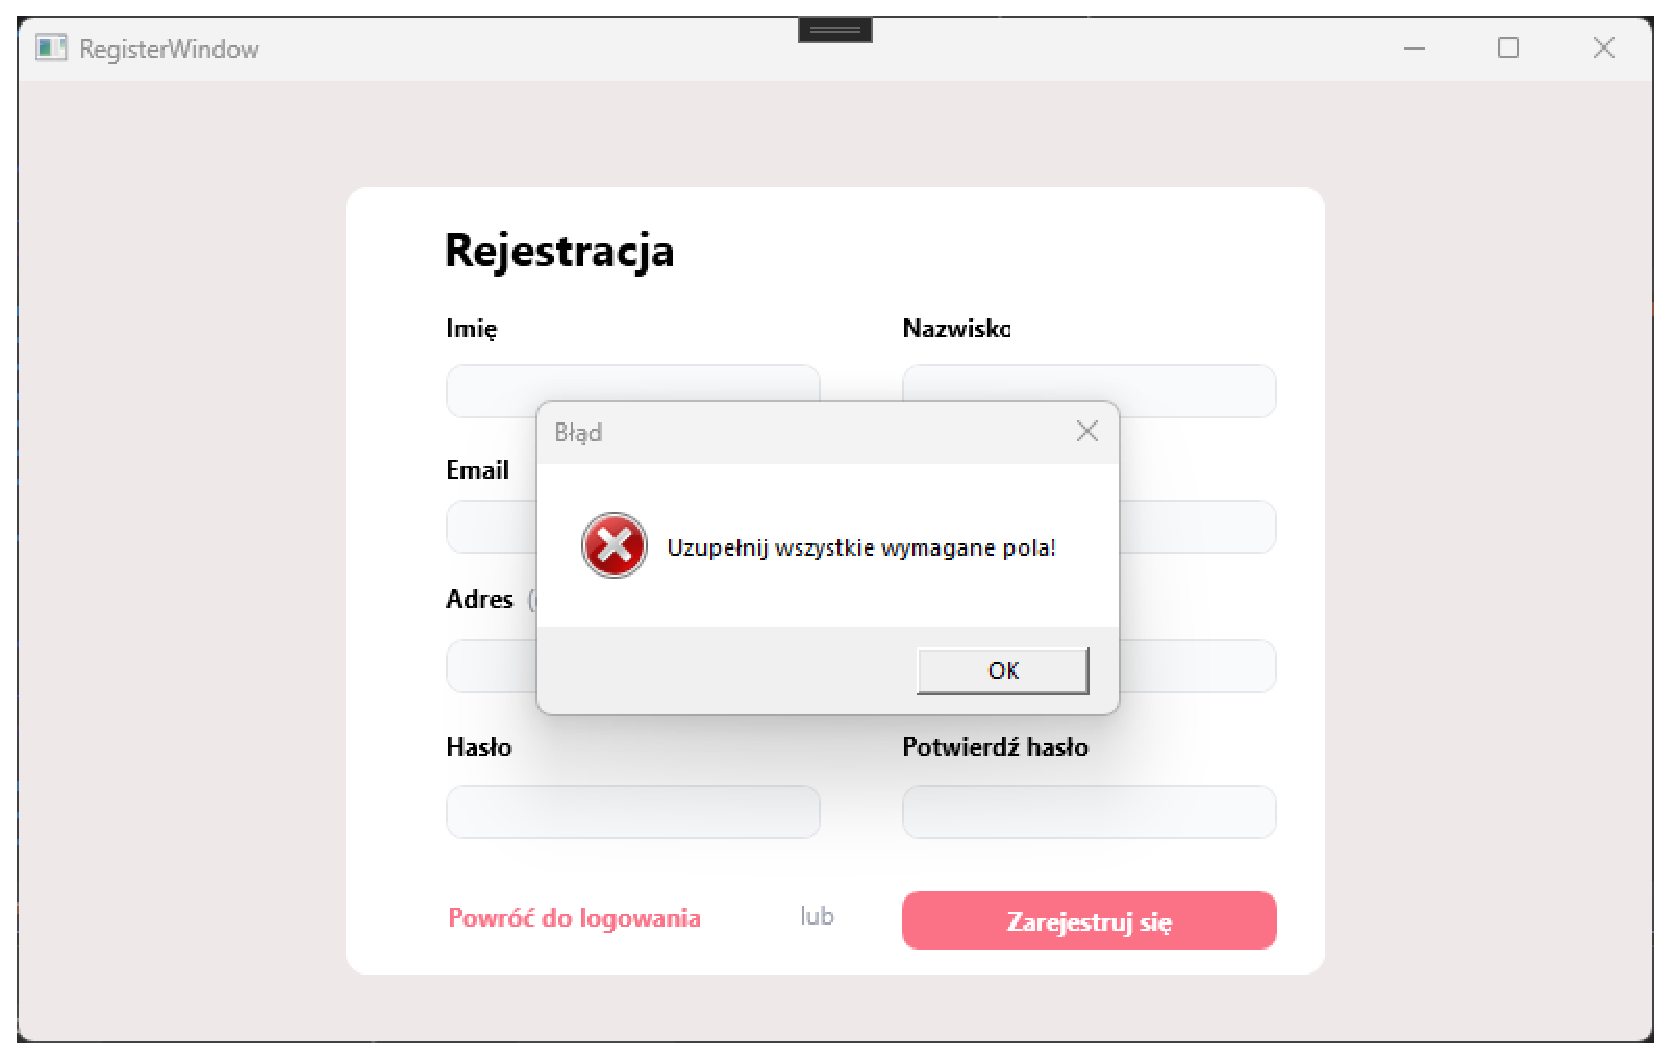
\includegraphics[width=0.8\linewidth]{figures/Rejestracja/fig_008.eps}
\caption{Komunikat błędu przy niewypełnionych polach formularza.\label{fig8}}
\end{figure}

Aplikacja weryfikuje również poprawność formatu numeru telefonu tzn. numer musi składać się z dokładnie 9 cyfr oraz nie zawierać innych znaków. 
W przypadku podania numeru w nieprawidłowym formacie wyświetlany jest odpowiedni komunikat błędu.

\begin{figure}[H]
\centering
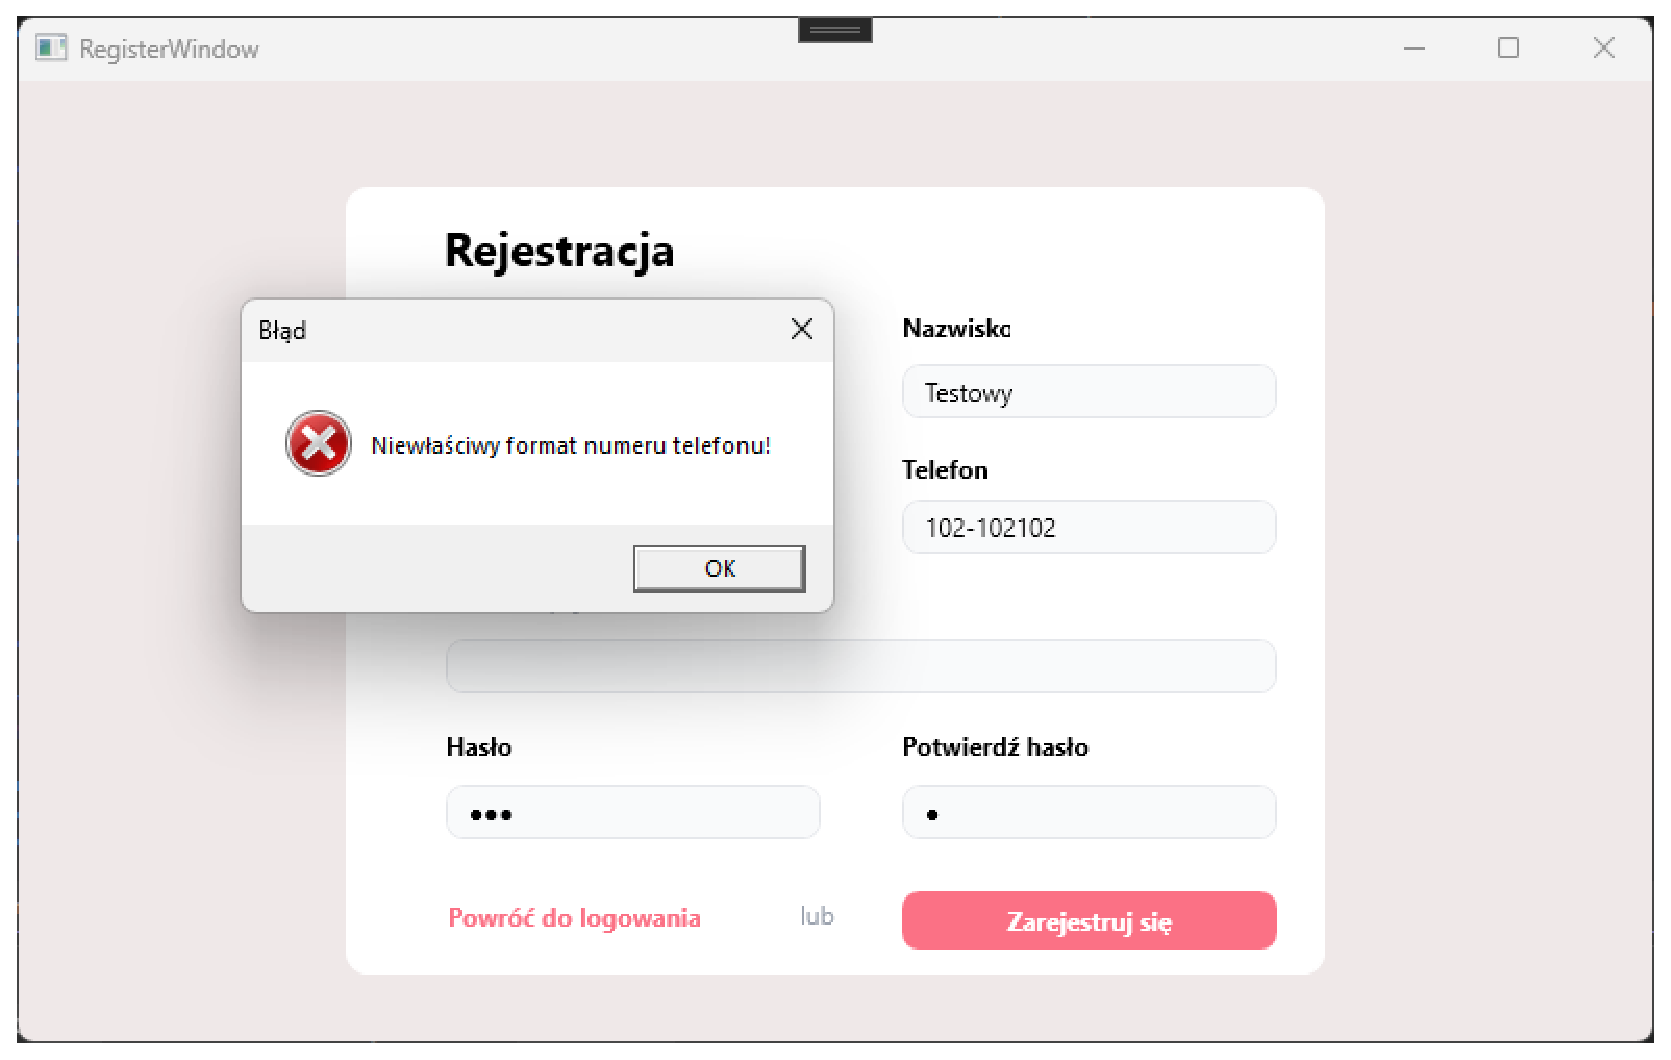
\includegraphics[width=0.8\linewidth]{figures/Rejestracja/fig_009.eps}
\caption{Komunikat błędu przy nieprawidłowym formacie numeru telefonu.\label{fig9}}
\end{figure}

Kolejnym etapem walidacji jest sprawdzenie, czy podane hasło i jego potwierdzenie są identyczne. W przypadku niezgodności haseł wyświetlany jest komunikat błędu.

\begin{figure}[H]
\centering
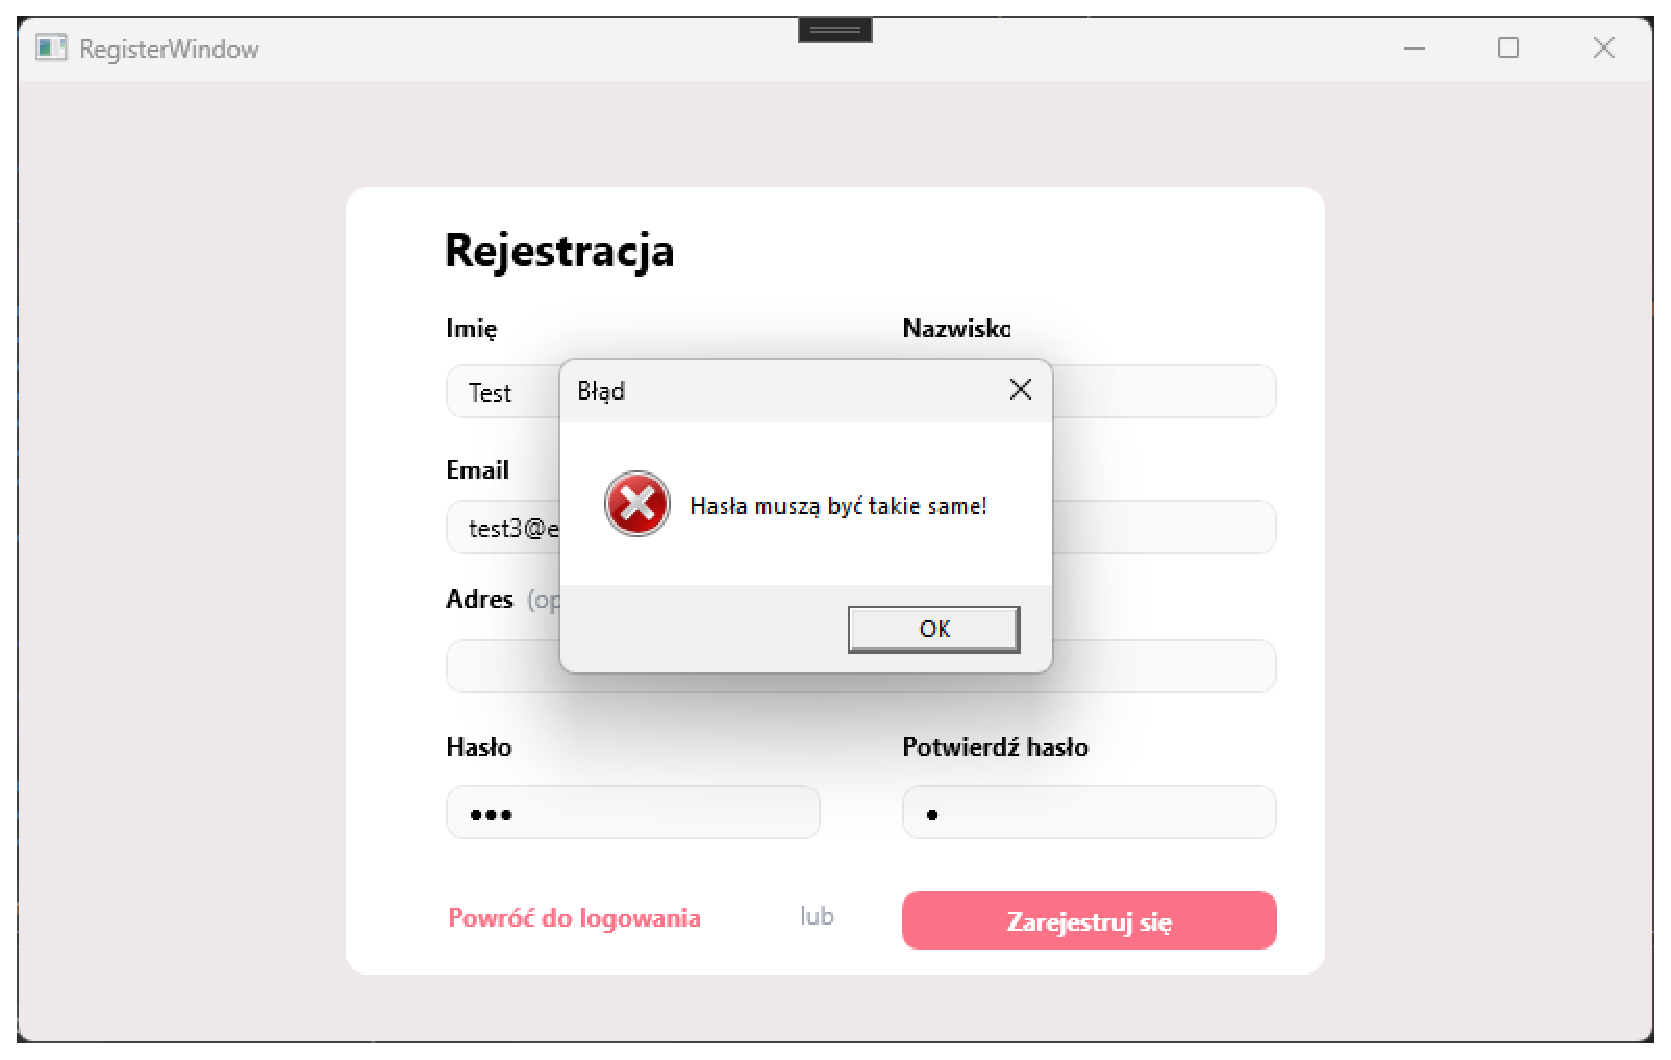
\includegraphics[width=0.8\linewidth]{figures/Rejestracja/fig_010.eps}
\caption{Komunikat błędu przy niezgodności haseł.\label{fig10}}
\end{figure}

Ostatnim etapem walidacji jest sprawdzenie długości hasła - musi ono zawierać co najmniej 6 znaków. W przypadku 
podania zbyt krótkiego hasła wyświetlany jest odpowiedni komunikat błędu.

\begin{figure}[H]
\centering
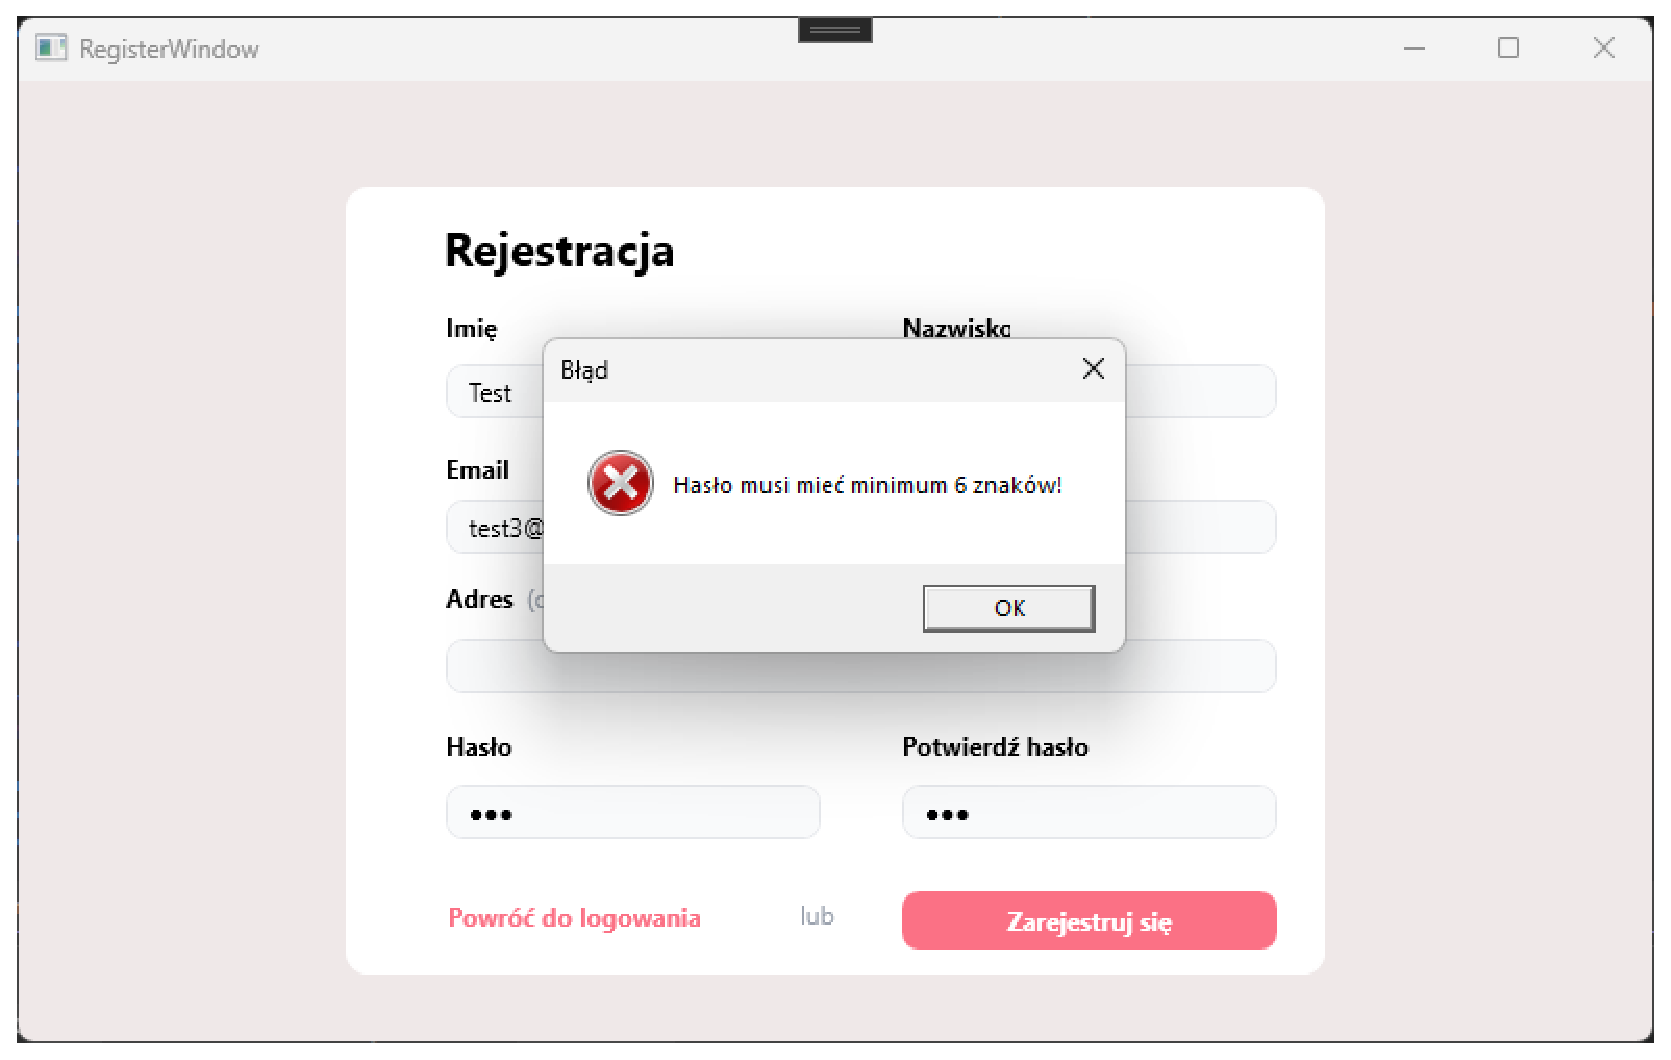
\includegraphics[width=0.8\linewidth]{figures/Rejestracja/fig_011.eps}
\caption{Komunikat błędu przy haśle krótszym niż 6 znaków.\label{fig11}}
\end{figure}

\section{Panel użytkownika}

\textbf{Zakładka "Moje konto"}

Zakładka "Moje konto" umożliwia zalogowanemu użytkownikowi przeglądanie i edycję swoich danych osobowych oraz 
zmianę hasła. W górnej części ekranu widoczny jest pasek nawigacyjny z nazwą kliniki, imieniem zalogowanego użytkownika, aktualnym 
saldem konta oraz przyciskiem wylogowania. Sekcja Twoje dane wyświetla imię, nazwisko, adres e-mail, numer telefonu 
oraz adres użytkownika wczytane automatycznie po zalogowaniu. Przycisk Zmień dane umożliwia zapisanie wprowadzonych zmian.

\begin{figure}[H]
\centering
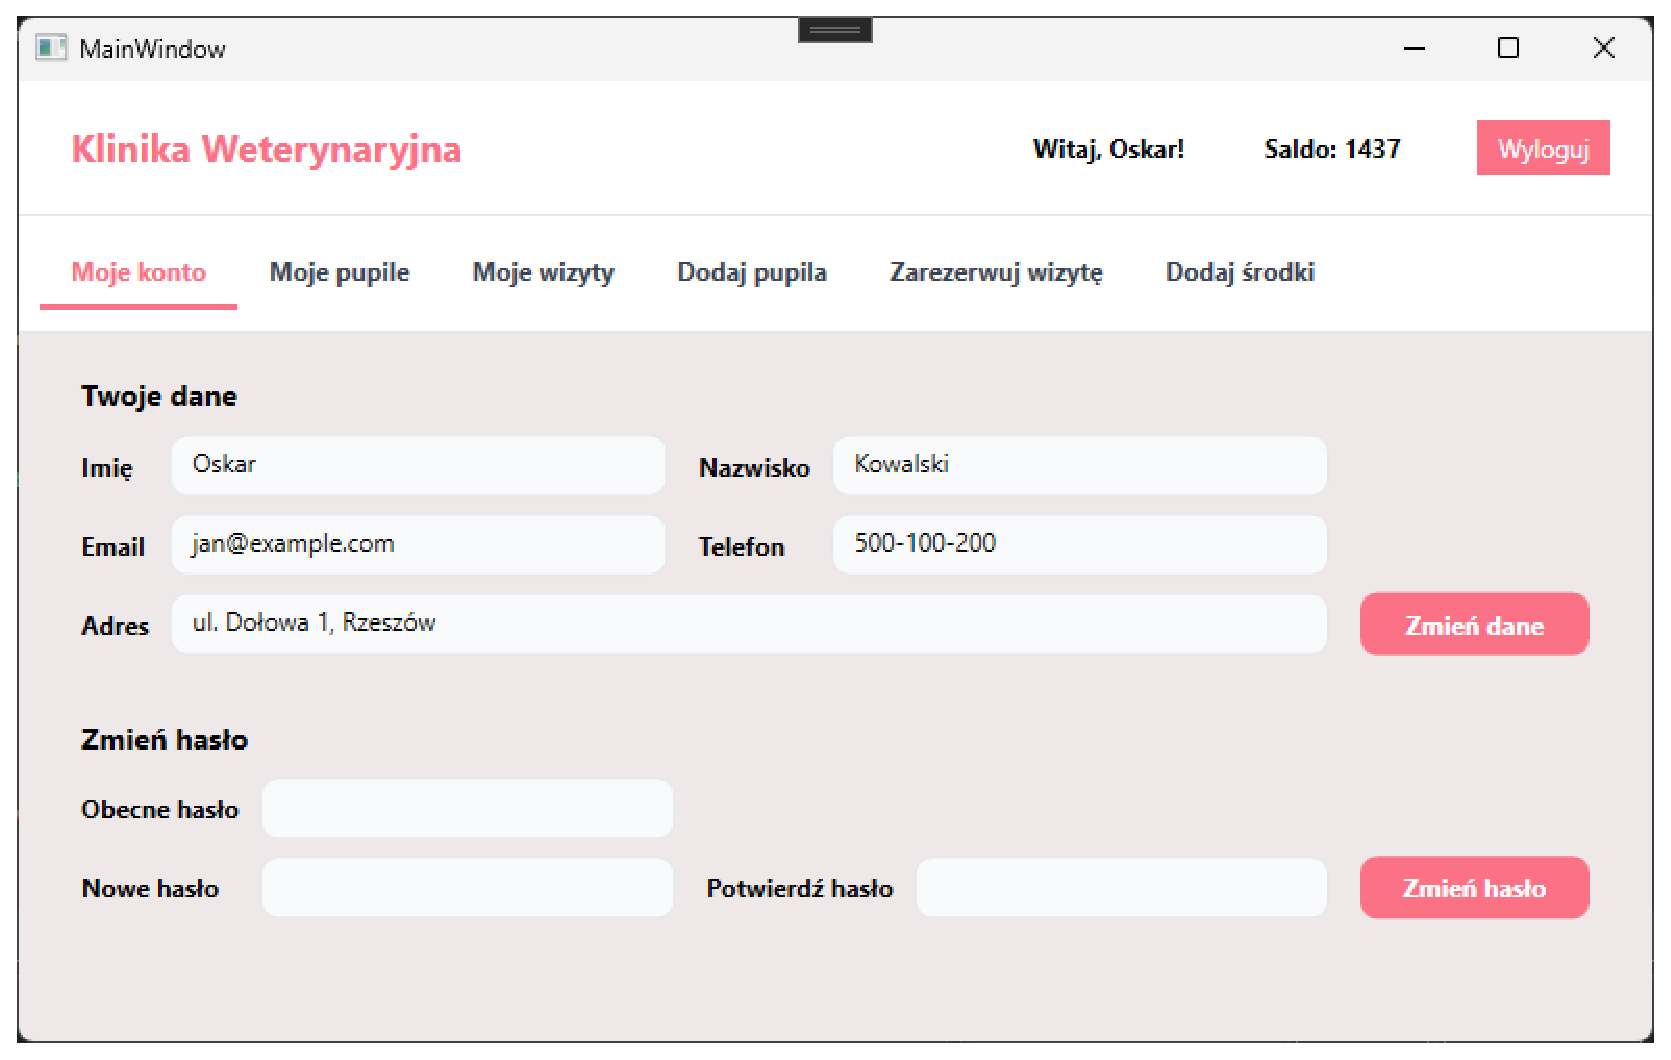
\includegraphics[width=0.9\linewidth]{figures/Uzytkownik/fig_012.eps}
\caption{Widok zakładki Moje konto.\label{fig12}}
\end{figure}

W przypadku kliknięcia przycisku Zmień dane bez wprowadzenia żadnych modyfikacji, aplikacja wyświetla 
komunikat informujący o konieczności wprowadzenia danych do zmiany.

\begin{figure}[H]
\centering
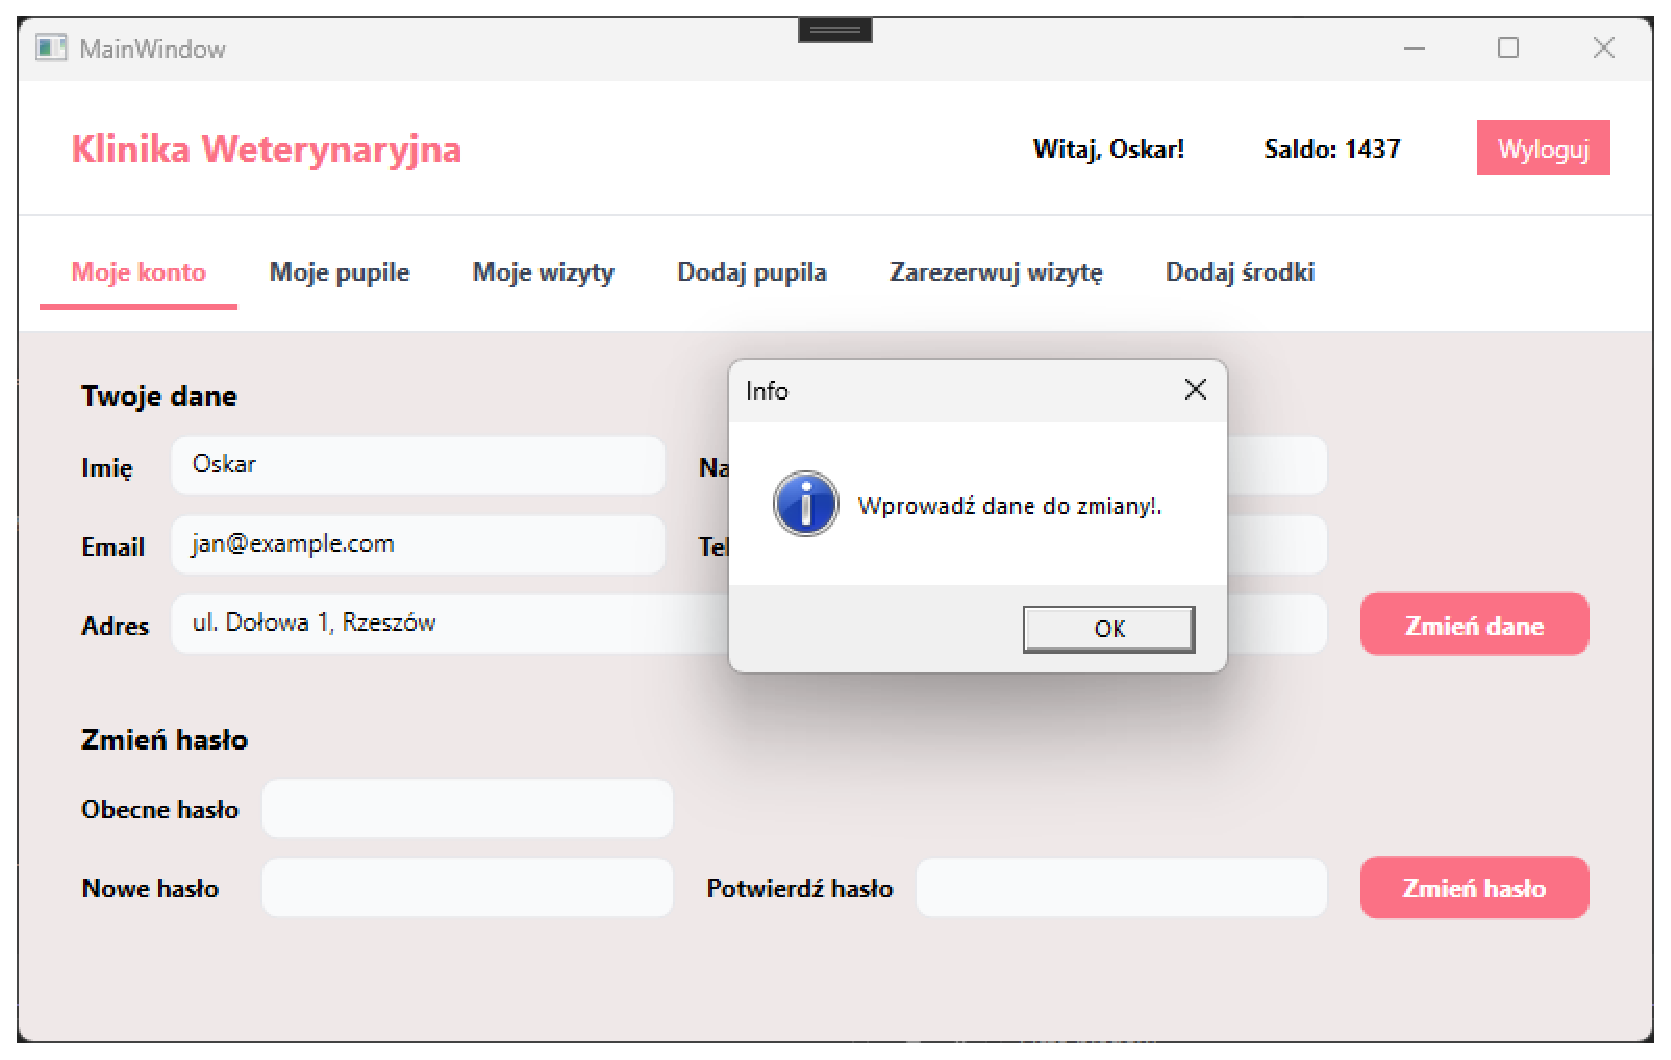
\includegraphics[width=0.9\linewidth]{figures/Uzytkownik/fig_013.eps}
\caption{Komunikat informacyjny przy braku zmian w danych.\label{fig13}}
\end{figure}

Sekcja Zmień hasło zawiera trzy pola: obecne hasło, nowe hasło oraz potwierdzenie nowego hasła. W przypadku gdy użytkownik nie wypełni wszystkich pól 
i kliknie przycisk Zmień hasło, wyświetlany jest komunikat błędu.

\begin{figure}[H]
\centering
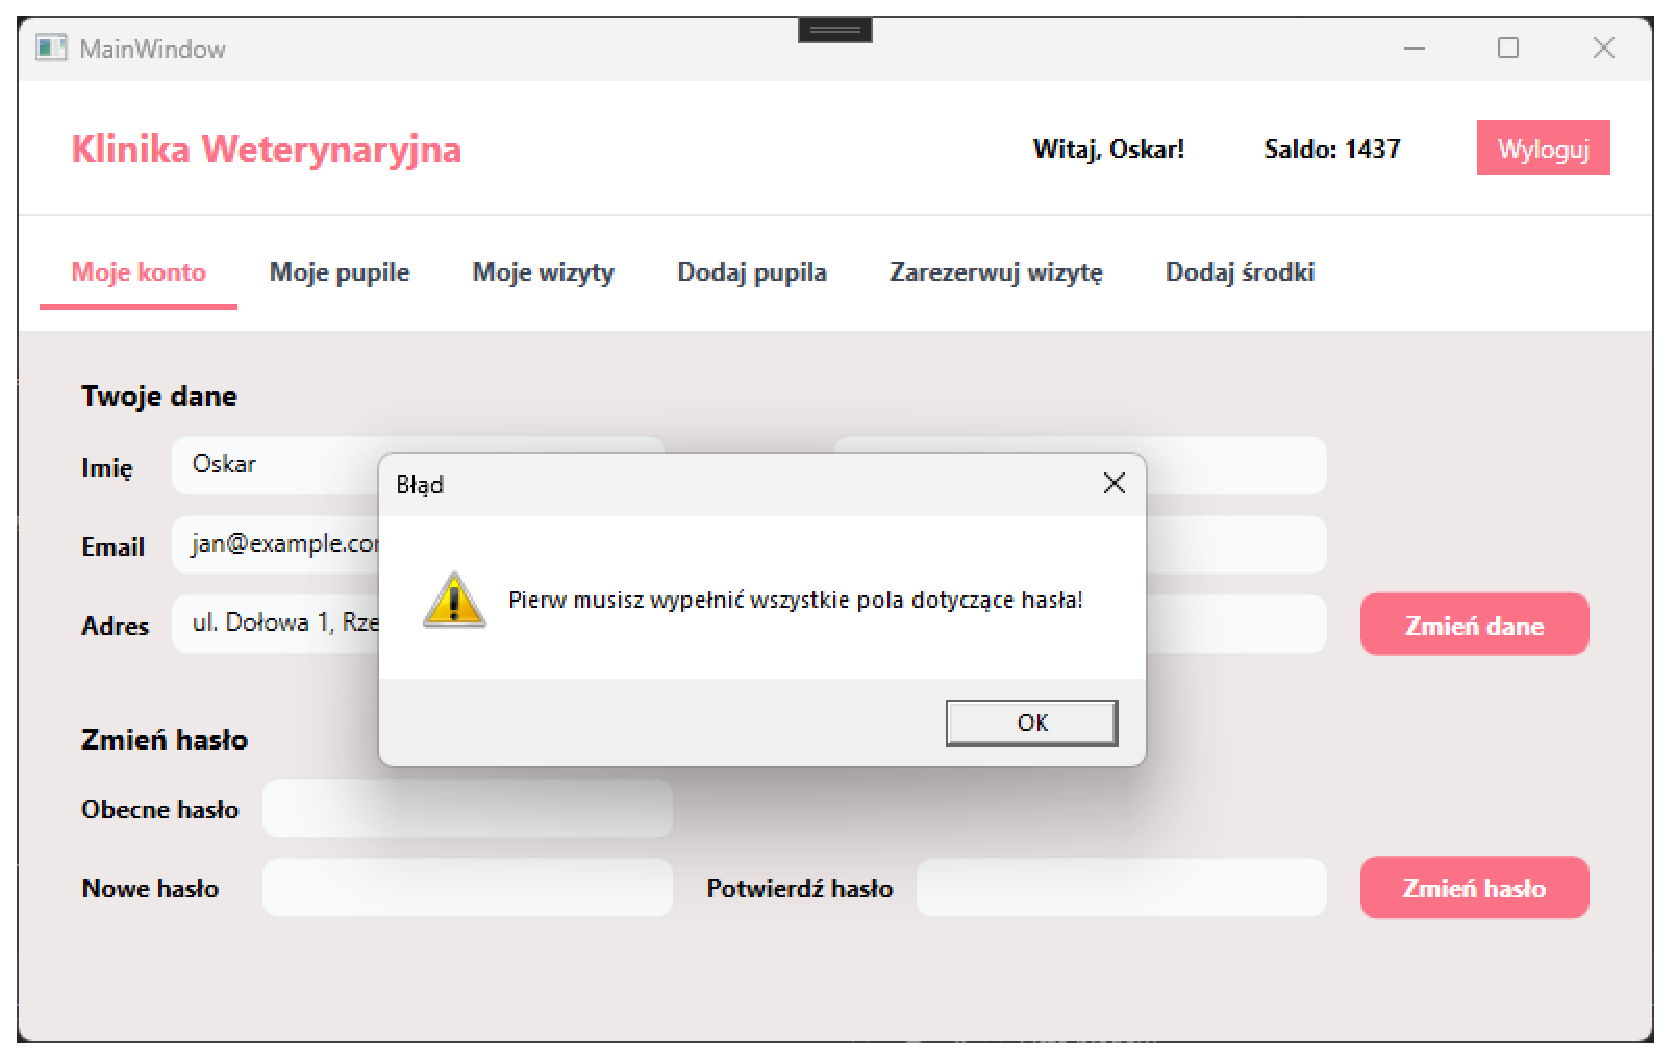
\includegraphics[width=0.9\linewidth]{figures/Uzytkownik/fig_014.eps}
\caption{Komunikat błędu przy niewypełnionych polach zmiany hasła.\label{fig14}}
\end{figure}

Aplikacja weryfikuje również poprawność obecnego hasła jeśli podane hasło nie zgadza się z aktualnym hasłem zapisanym
w systemie, wyświetlany jest komunikat błędu.

\begin{figure}[H]
\centering
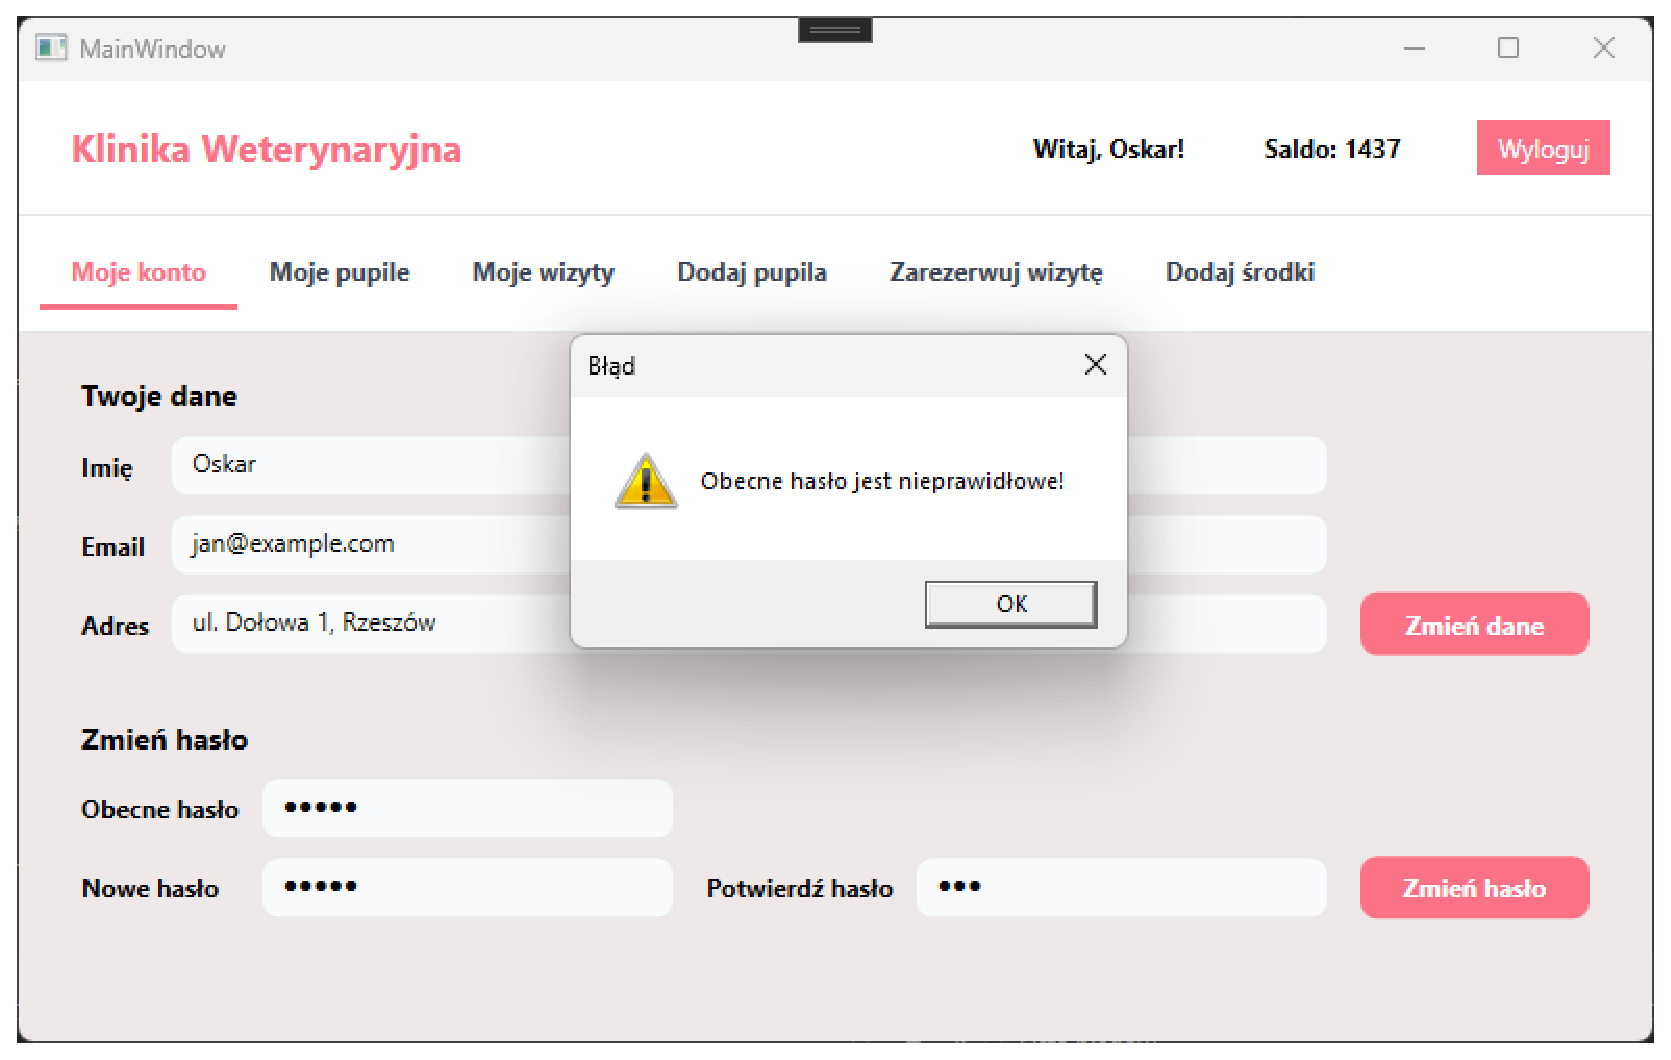
\includegraphics[width=0.9\linewidth]{figures/Uzytkownik/fig_015.eps}
\caption{Komunikat błędu przy nieprawidłowym obecnym haśle.\label{fig15}}
\end{figure}

Kolejnym etapem walidacji jest sprawdzenie zgodności nowego hasła z polem potwierdzającym oraz sprawdzenie czy hasło ma co najmniej 6 znaków. 
W przypadku niezgodności lub zbyt krótkiego hasła wyświetlane są odpowiednie komunikaty błędów.

\begin{figure}[H]
\centering
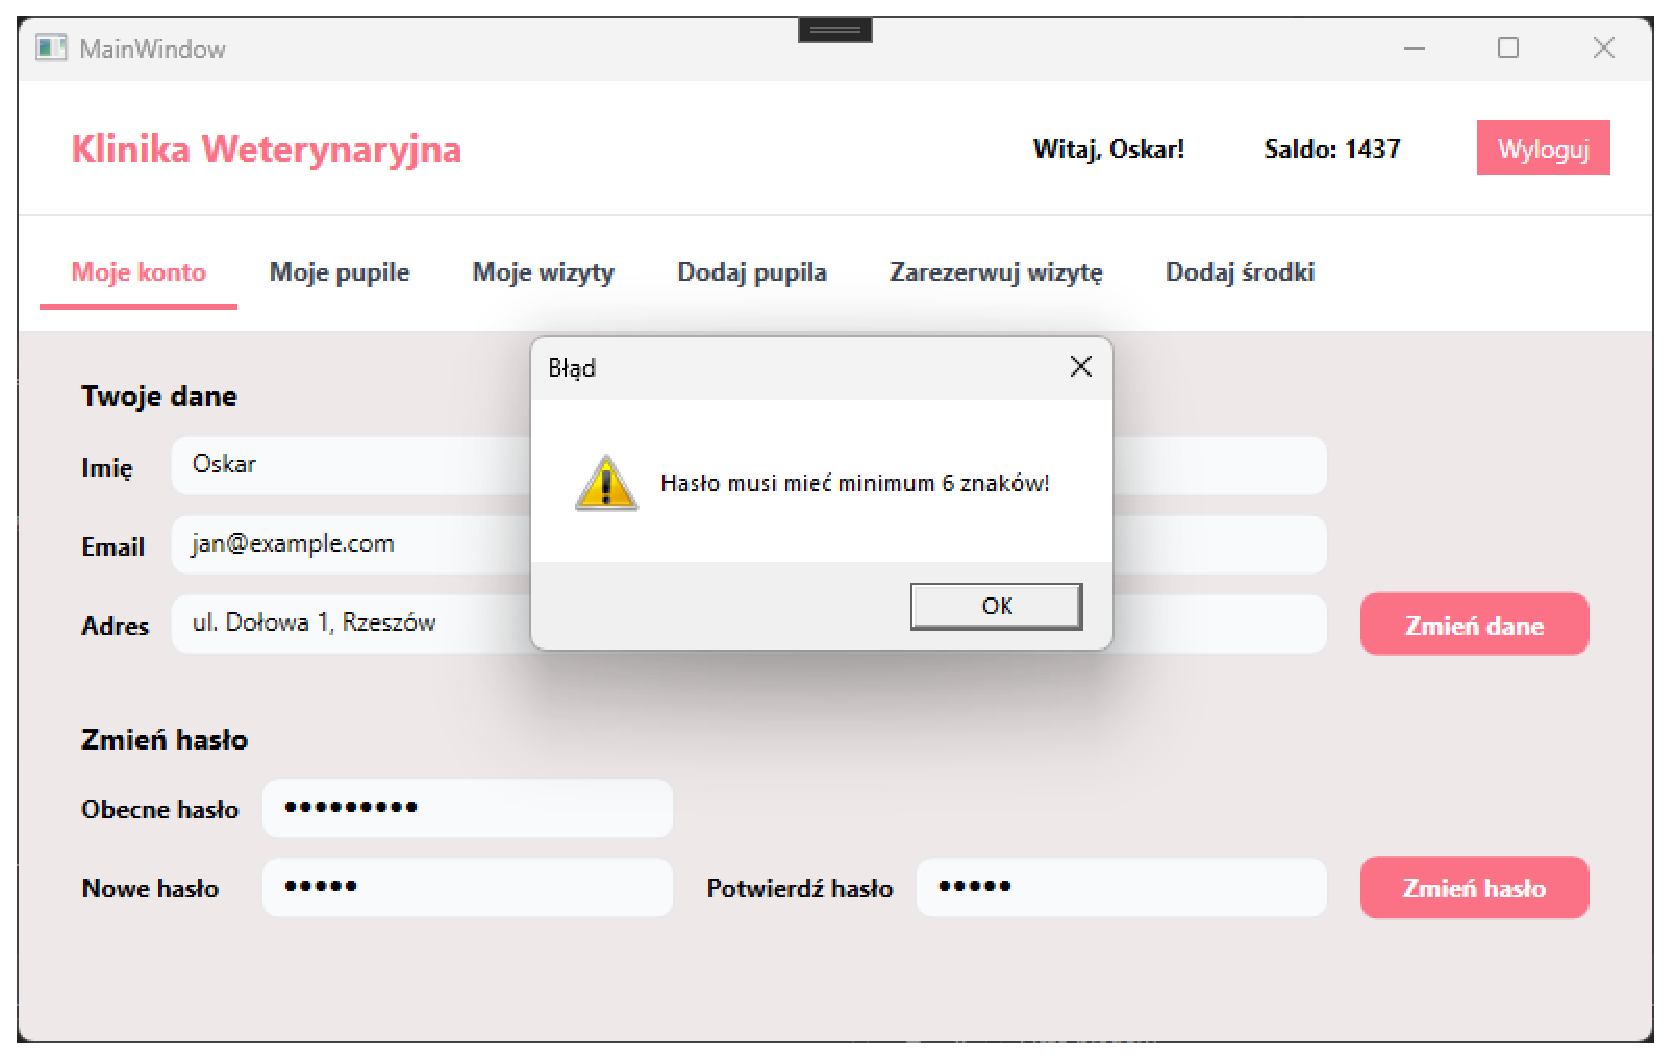
\includegraphics[width=0.9\linewidth]{figures/Uzytkownik/fig_016.eps}
\caption{Komunikat błędu przy niezgodności nowych haseł.\label{fig16}}
\end{figure}

\begin{figure}[H]
\centering
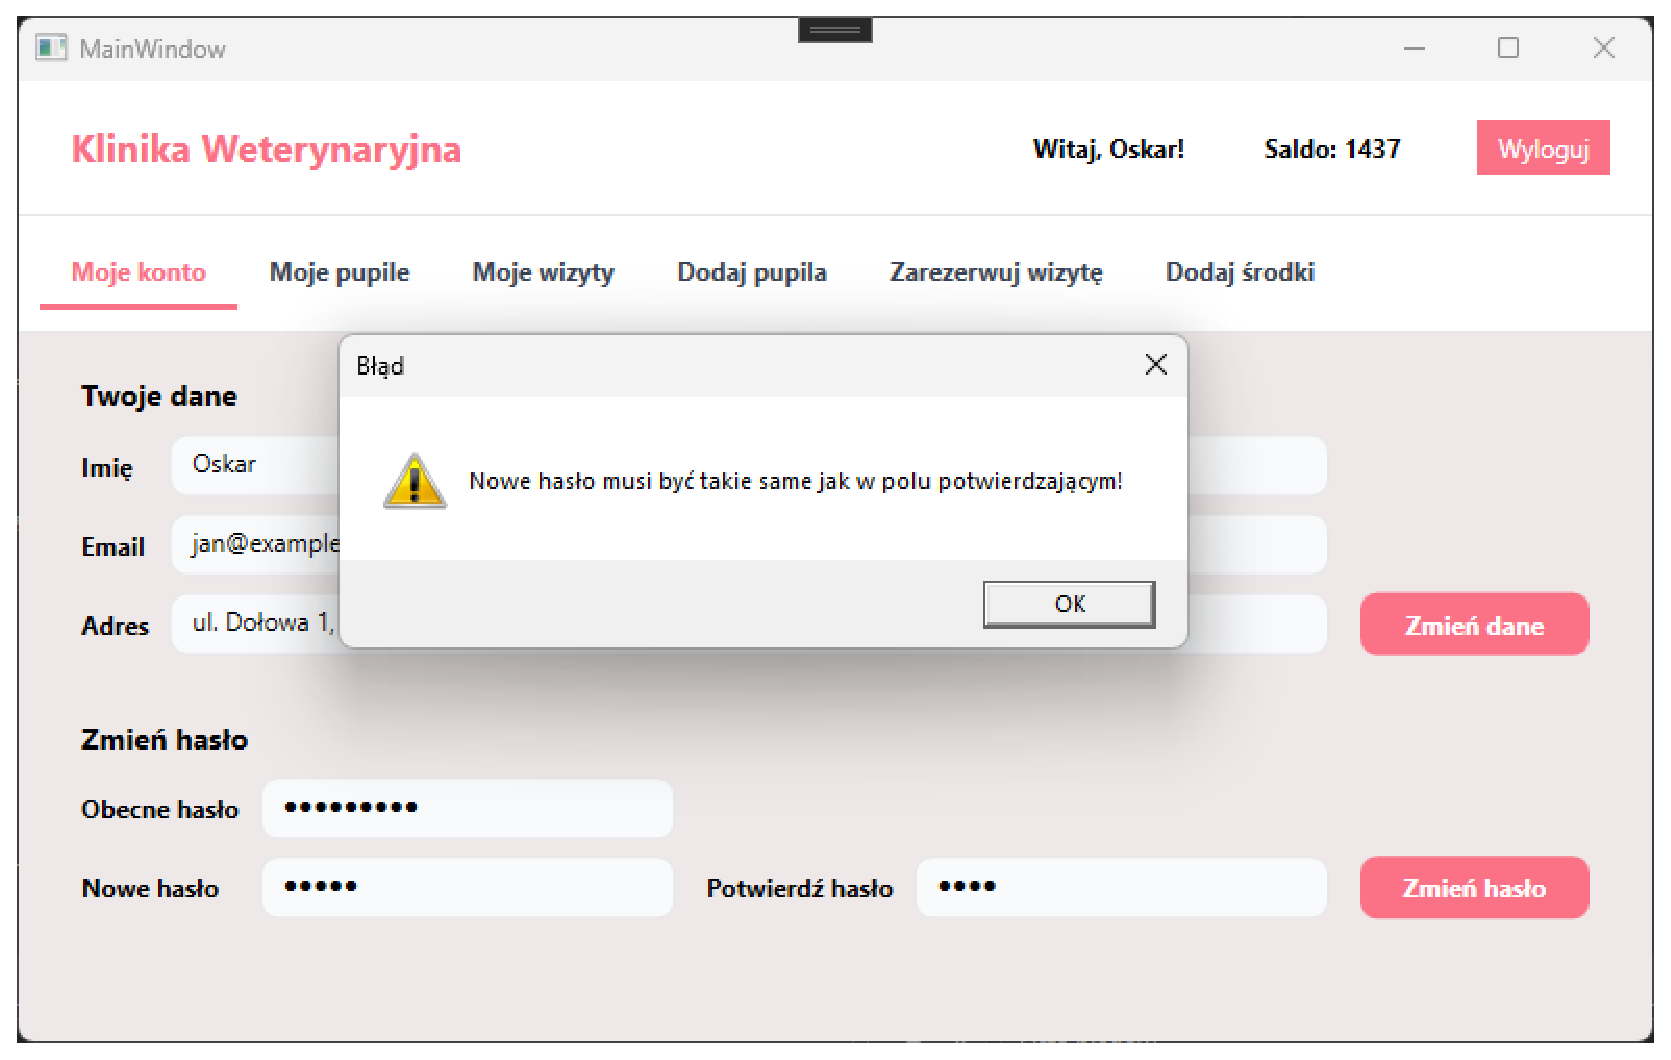
\includegraphics[width=0.9\linewidth]{figures/Uzytkownik/fig_017.eps}
\caption{Komunikat błędu przy haśle krótszym niż 6 znaków.\label{fig17}}
\end{figure}

\textbf{Zakładka "Moje pupile"}

Zakładka "Moje pupile" wyświetla listę wszystkich pupili przypisanych do zalogowanego użytkownika. Dla każdego pupila 
prezentowane są informacje takie jak imię, gatunek, rasa, wiek oraz płeć. Przy każdym pupilu dostępne 
dwa przyciski: Edytuj wiek umożliwiający zmianę wieku pupila oraz Usuń umożliwiający usunięcie pupila z systemu.

\begin{figure}[H]
\centering
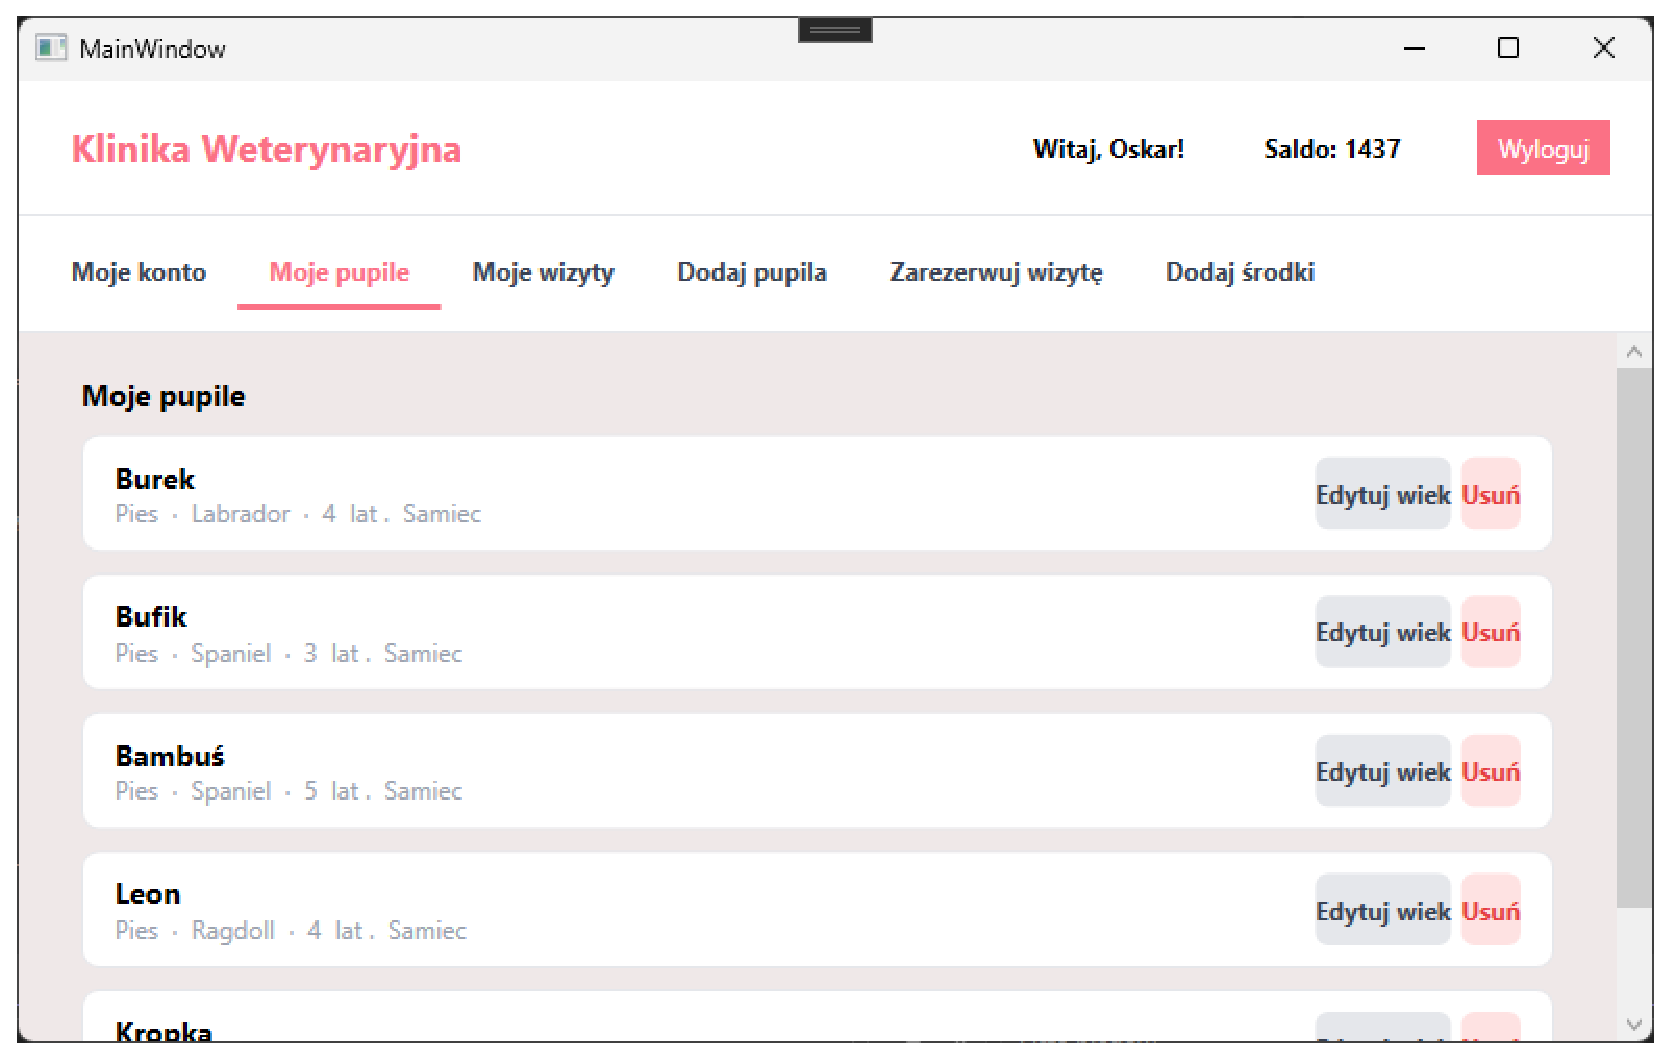
\includegraphics[width=0.9\linewidth]{figures/Uzytkownik/fig_018.eps}
\caption{Widok zakładki Moje pupile.\label{fig18}}
\end{figure}

Po kliknięciu przycisku Edytuj wiek otwierane jest okno dialogowe z polem tekstowym, w którym użytkownik może wprowadzić nowy wiek pupila. 
Zmiana zostaje zapisana po kliknięciu przycisku Zapisz.

\begin{figure}[H]
\centering
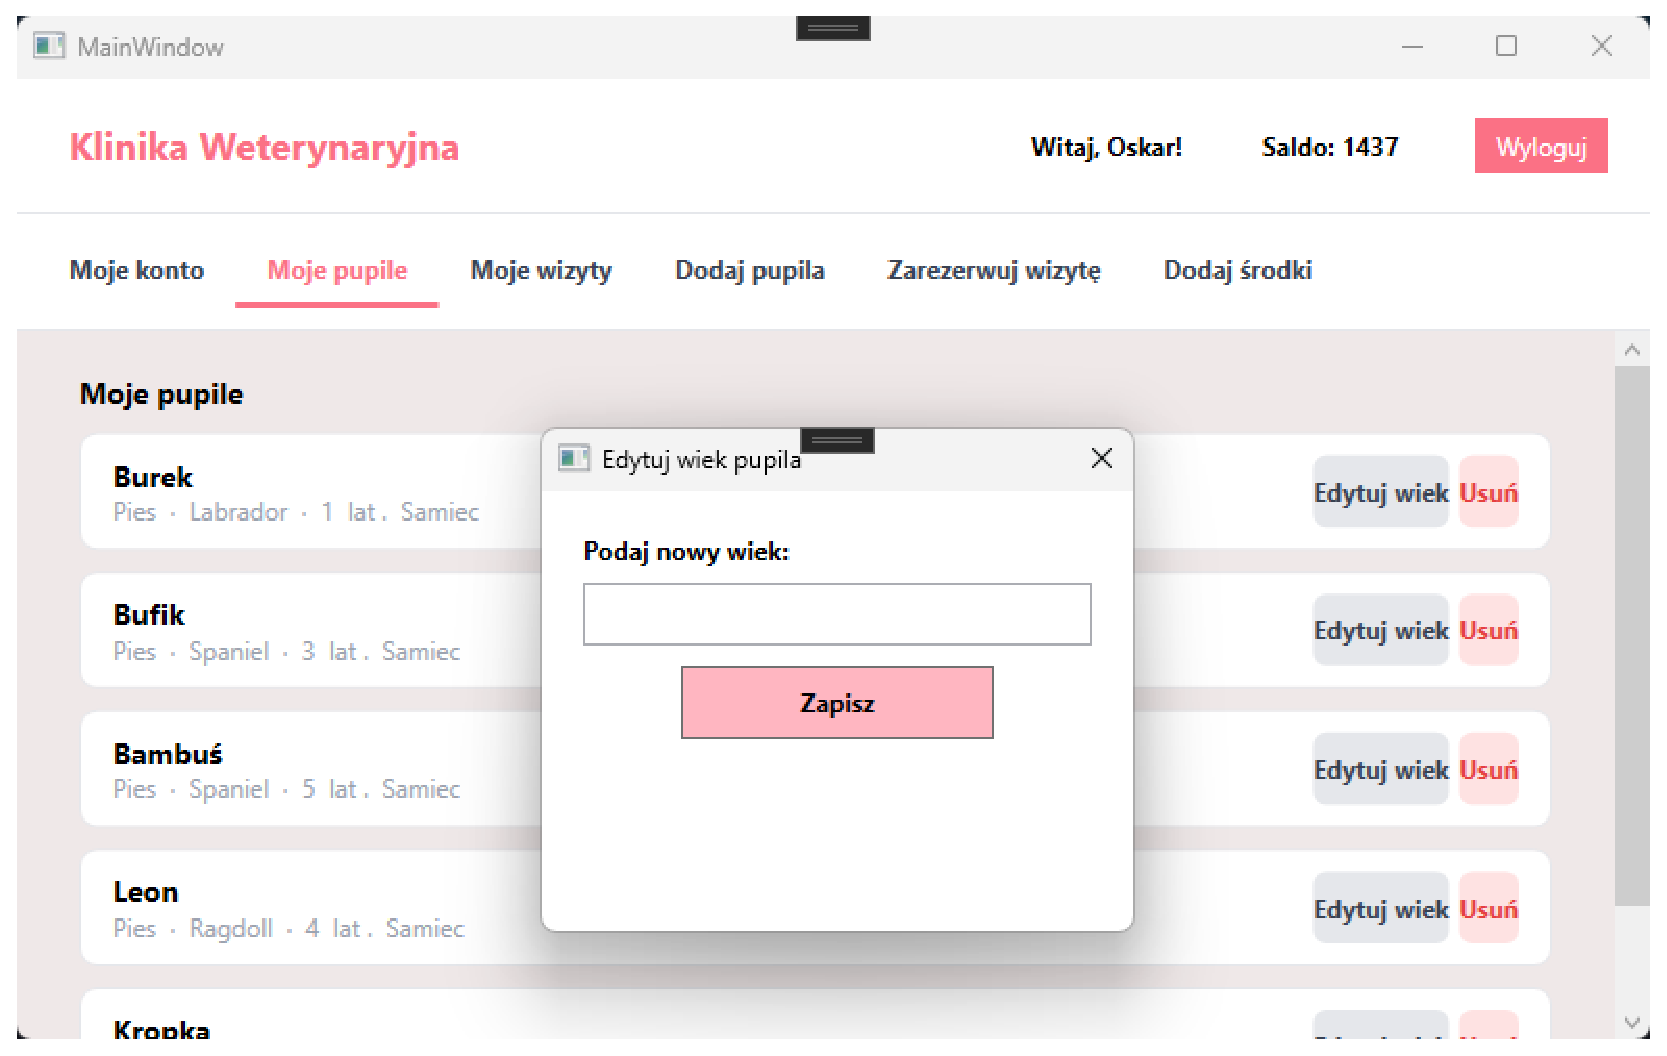
\includegraphics[width=0.9\linewidth]{figures/Uzytkownik/fig_019.eps}
\caption{Okno dialogowe edycji wieku pupila.\label{fig19}}
\end{figure}

W przypadku podania nieprawidłowej wartości wieku aplikacja wyświetla komunikat błędu informujący o konieczności podania prawidłowej wartości.

\begin{figure}[H]
\centering
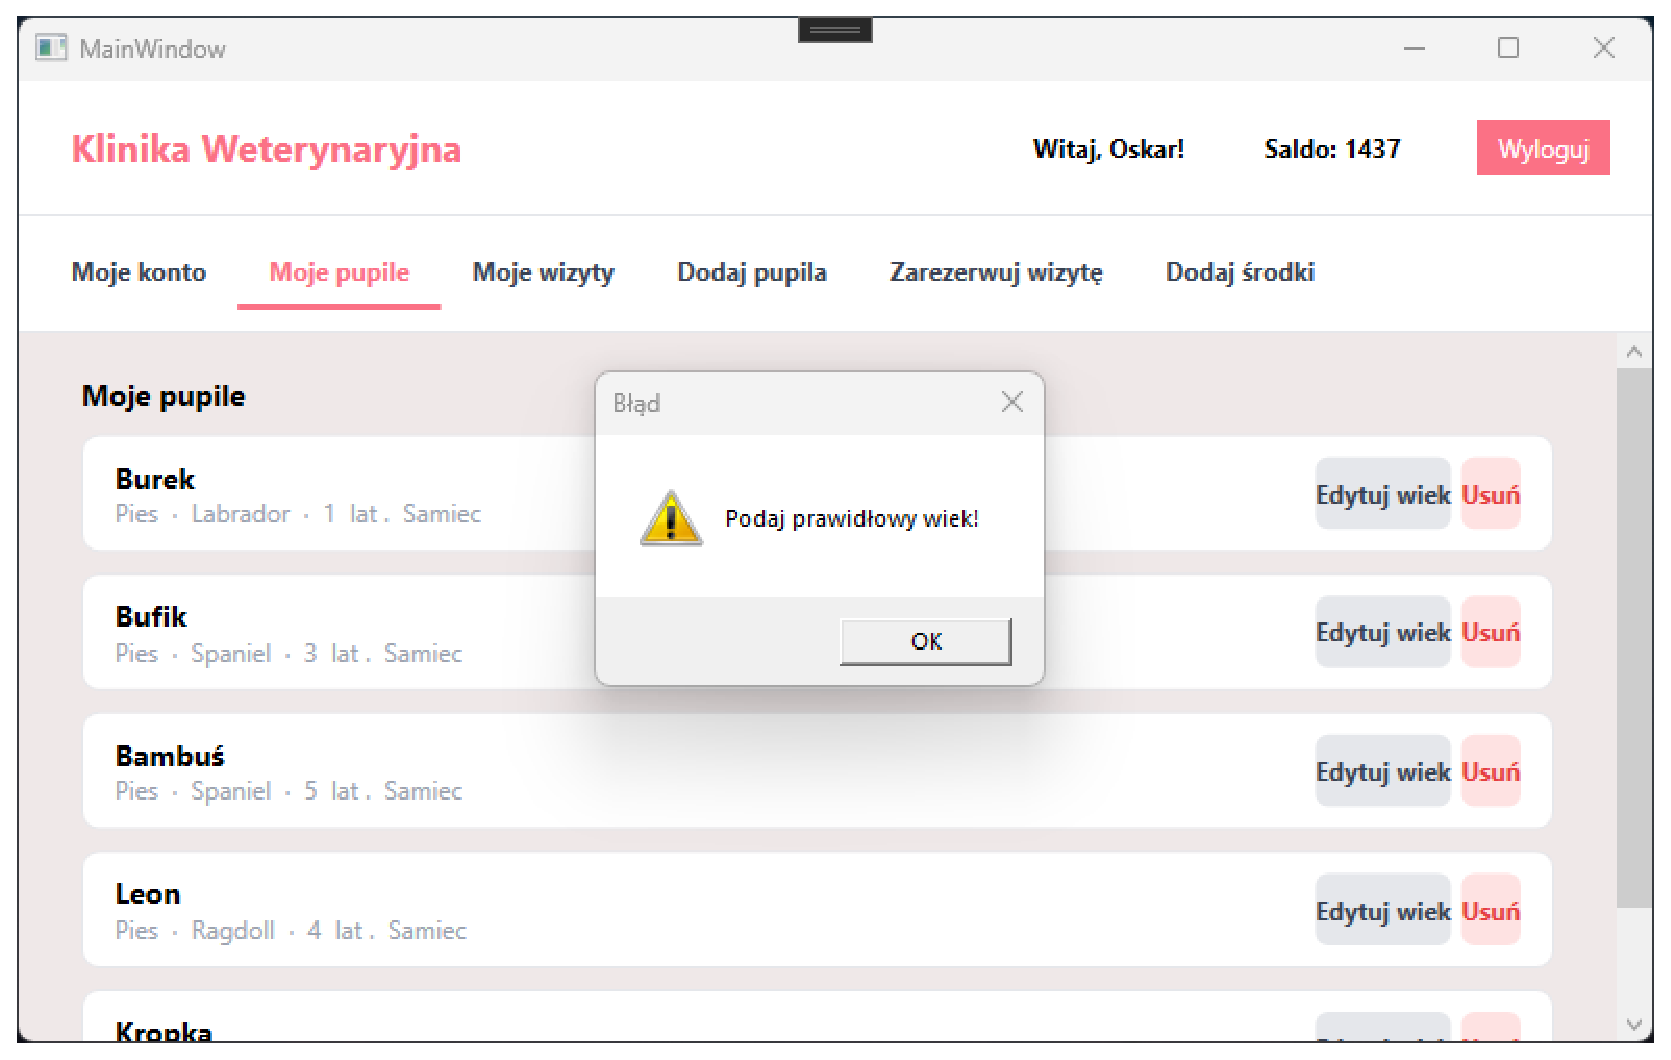
\includegraphics[width=0.9\linewidth]{figures/Uzytkownik/fig_020.eps}
\caption{Komunikat błędu przy nieprawidłowym wieku pupila.\label{fig20}}
\end{figure}

Po kliknięciu przycisku Usuń aplikacja wyświetla okno dialogowe z prośbą o potwierdzenie operacji. 
Po potwierdzeniu pupil zostaje usunięty z systemu wraz z jego rezerwacjami, a lista pupili jest automatycznie odświeżana.

\begin{figure}[H]
\centering
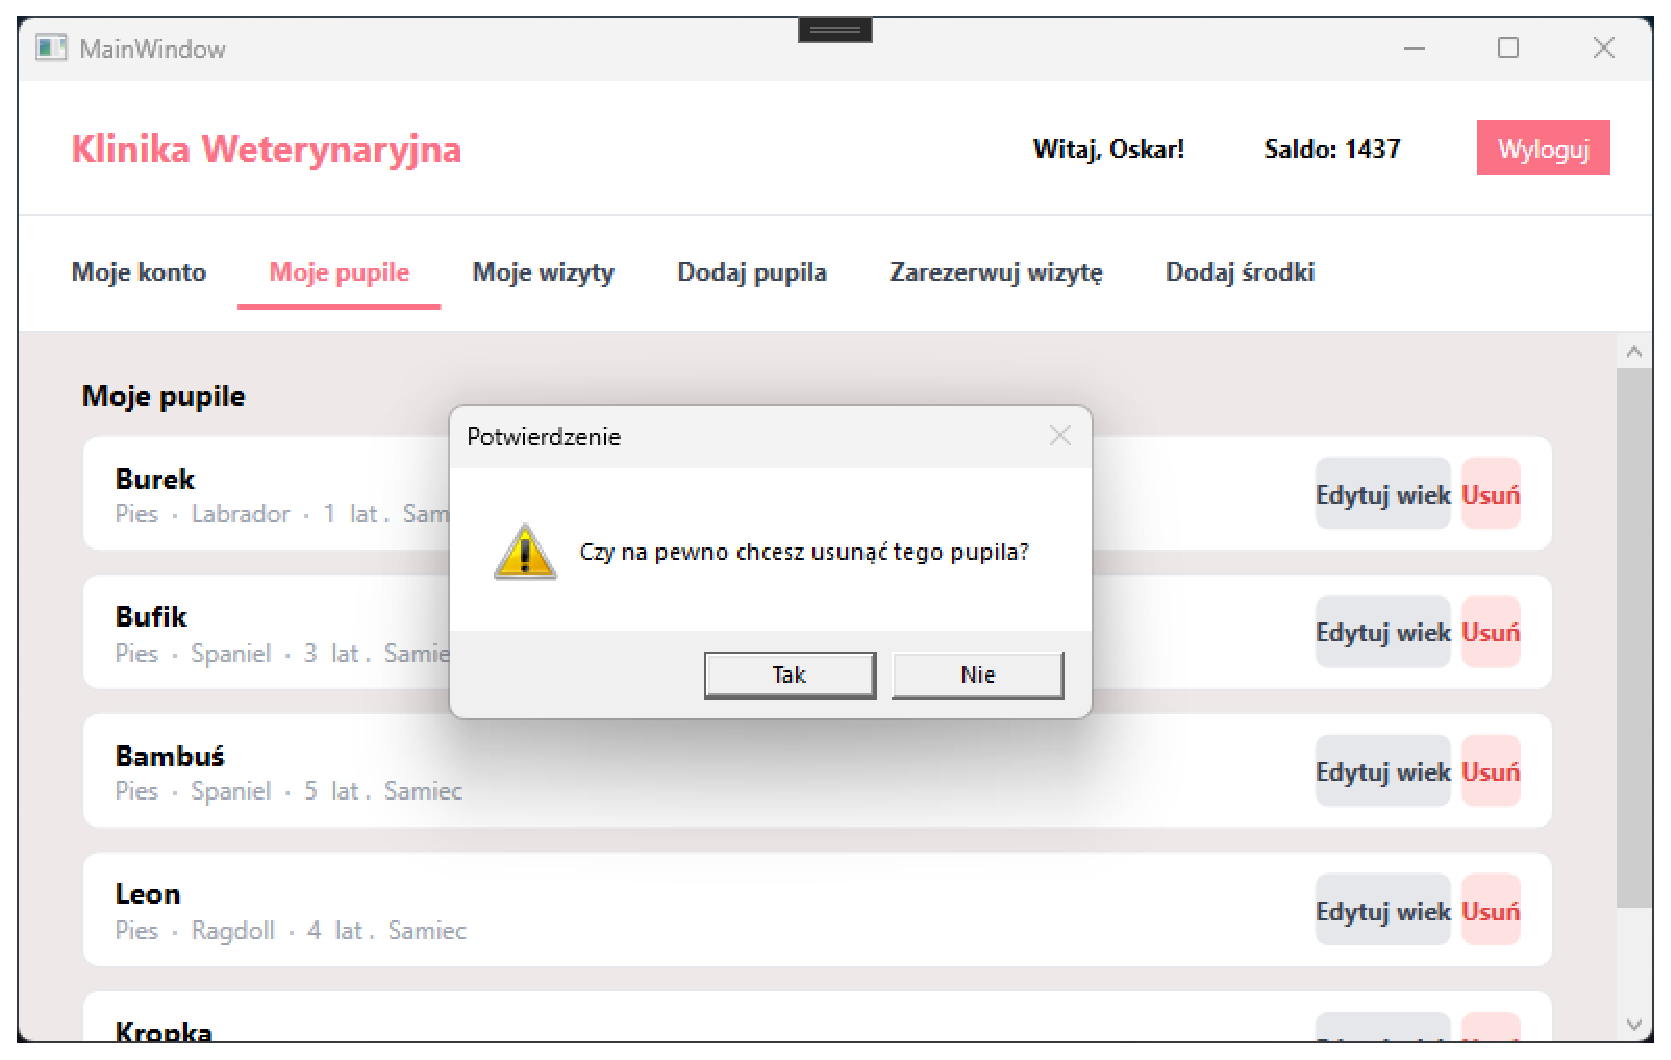
\includegraphics[width=0.9\linewidth]{figures/Uzytkownik/fig_021.eps}
\caption{Okno potwierdzenia usunięcia pupila.\label{fig21}}
\end{figure}

\textbf{Zakładka "Moje wizyty"}

Zakładka "Moje Wizyty" wyświetla historię wszystkich rezerwacji wizyt zalogowanego użytkownika. Dla każdej wizyty prezentowane 
są informacje takie jak nazwa zabiegu, imię pupila, data, godziny wizyty oraz imię i nazwisko weterynarza. Każda wizyta oznaczona 
jest kolorowym znacznikiem statusu: zielonym dla wizyt zarezerwowanych, szarym dla anulowanych oraz ciemnozielonym dla zrealizowanych. 
Przy każdej wizycie dostępny jest przycisk Anuluj umożliwiający anulowanie rezerwacji.

\begin{figure}[H]
\centering
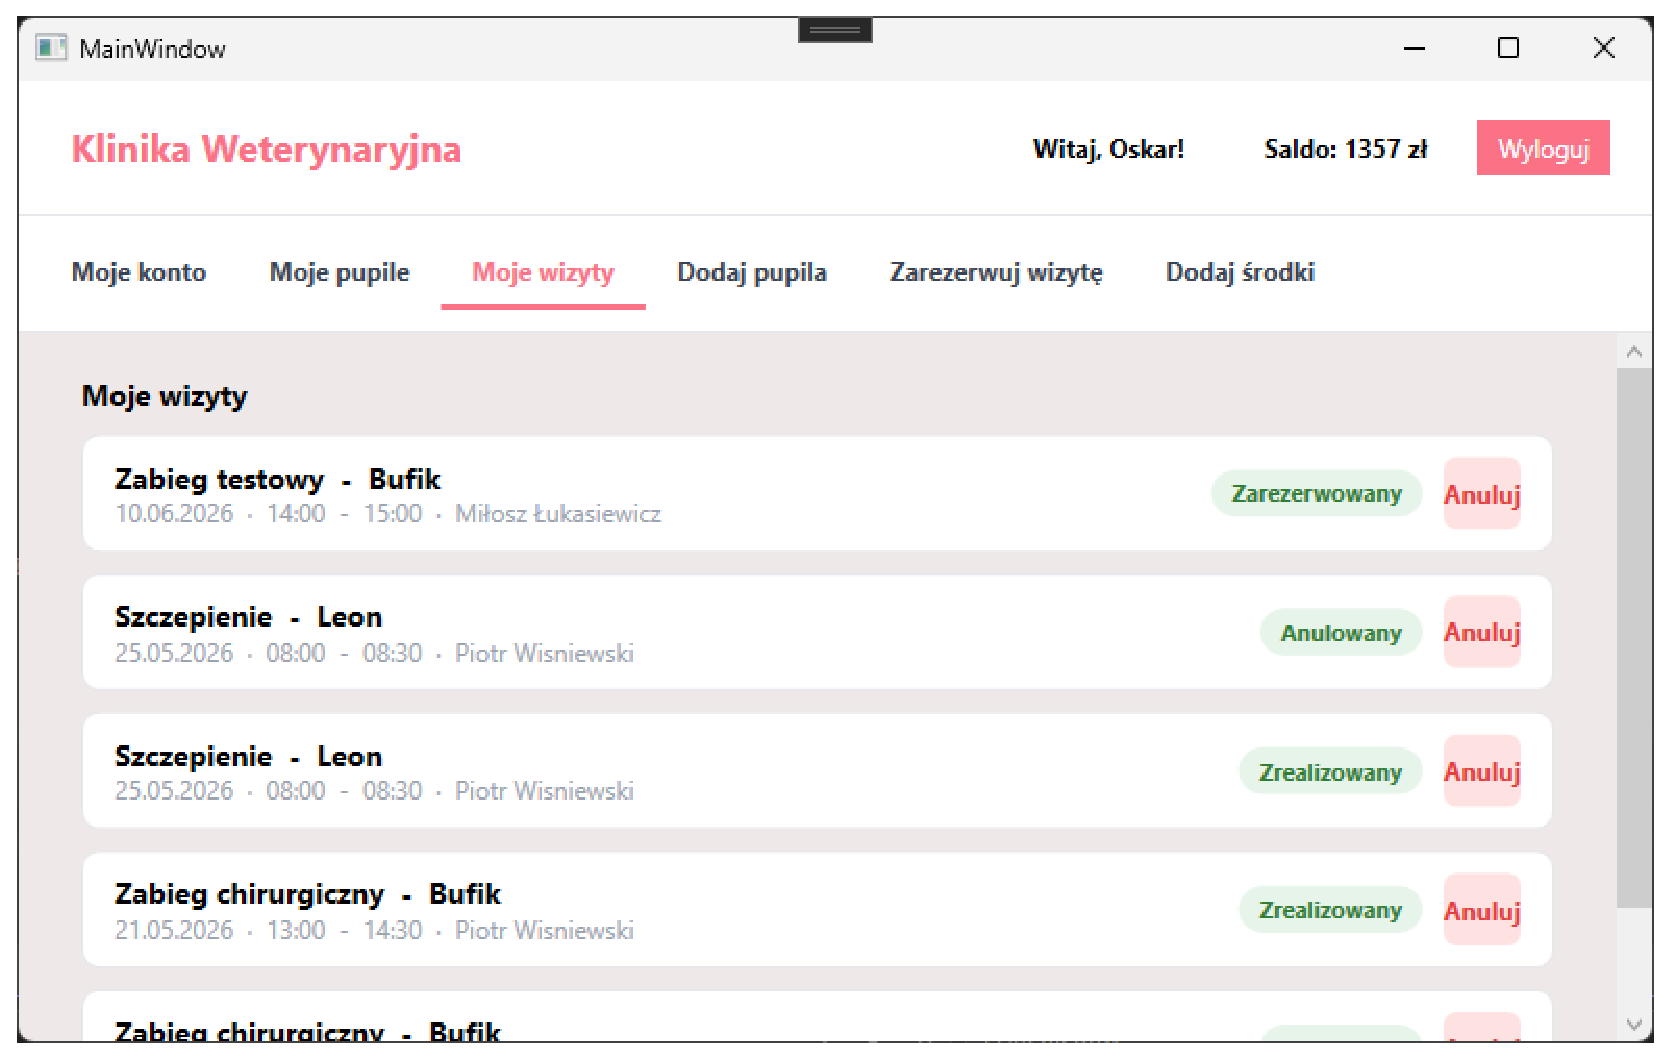
\includegraphics[width=0.9\linewidth]{figures/Uzytkownik/fig_022.eps}
\caption{Widok zakładki Moje wizyty.\label{fig22}}
\end{figure}

Po kliknięciu przycisku Anuluj aplikacja wyświetla okno dialogowe z prośbą o potwierdzenie operacji. 
Po potwierdzeniu status wizyty zostaje zmieniony na Anulowany, a lista wizyt jest automatycznie odświeżana.

\begin{figure}[H]
\centering
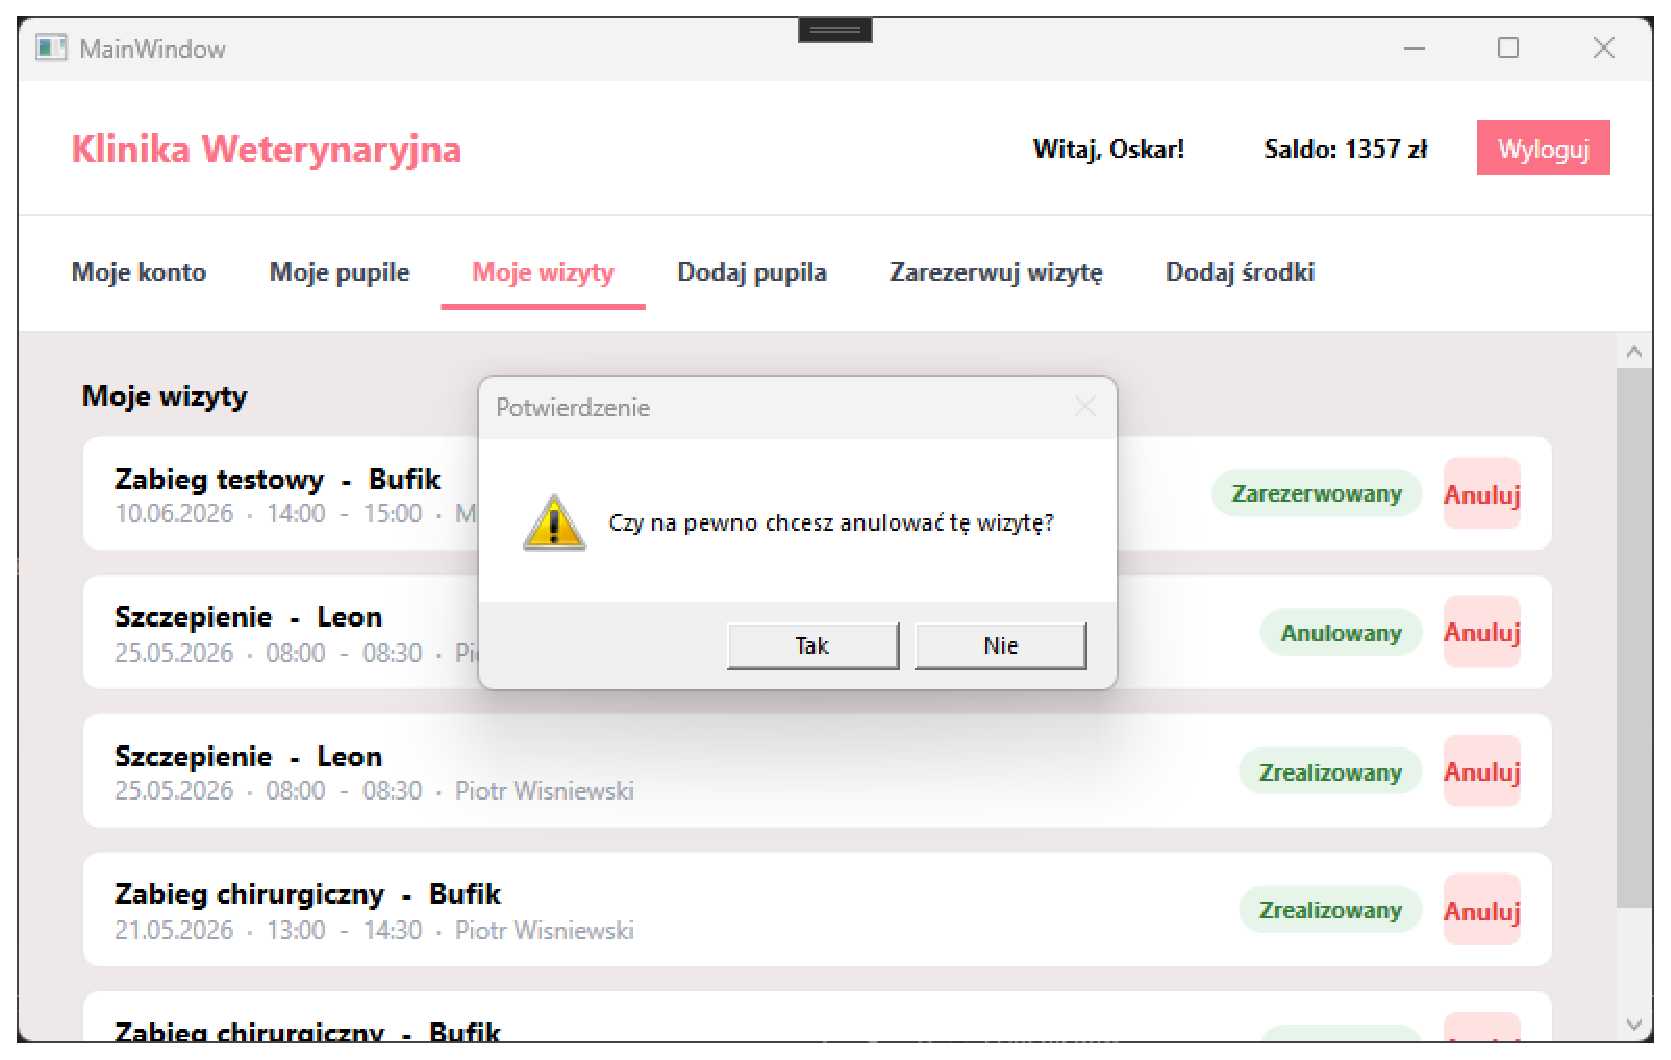
\includegraphics[width=0.9\linewidth]{figures/Uzytkownik/fig_023.eps}
\caption{Okno potwierdzenia anulowania wizyty.\label{fig23}}
\end{figure}

\textbf{Okno "Dodaj pupila"}

Okno "Dodaj pupila" otwierane jest po kliknięciu przycisku Dodaj pupila w pasku nawigacyjnym. Formularz zawiera pola: imię, 
gatunek (lista rozwijana z opcjami Pies i Kot), rasa, wiek w latach oraz płeć (lista rozwijana z opcjami Samiec i Samica). 
Po wypełnieniu formularza i kliknięciu przycisku Dodaj Pupila aplikacja przeprowadza walidację wprowadzonych danych.

\begin{figure}[H]
\centering
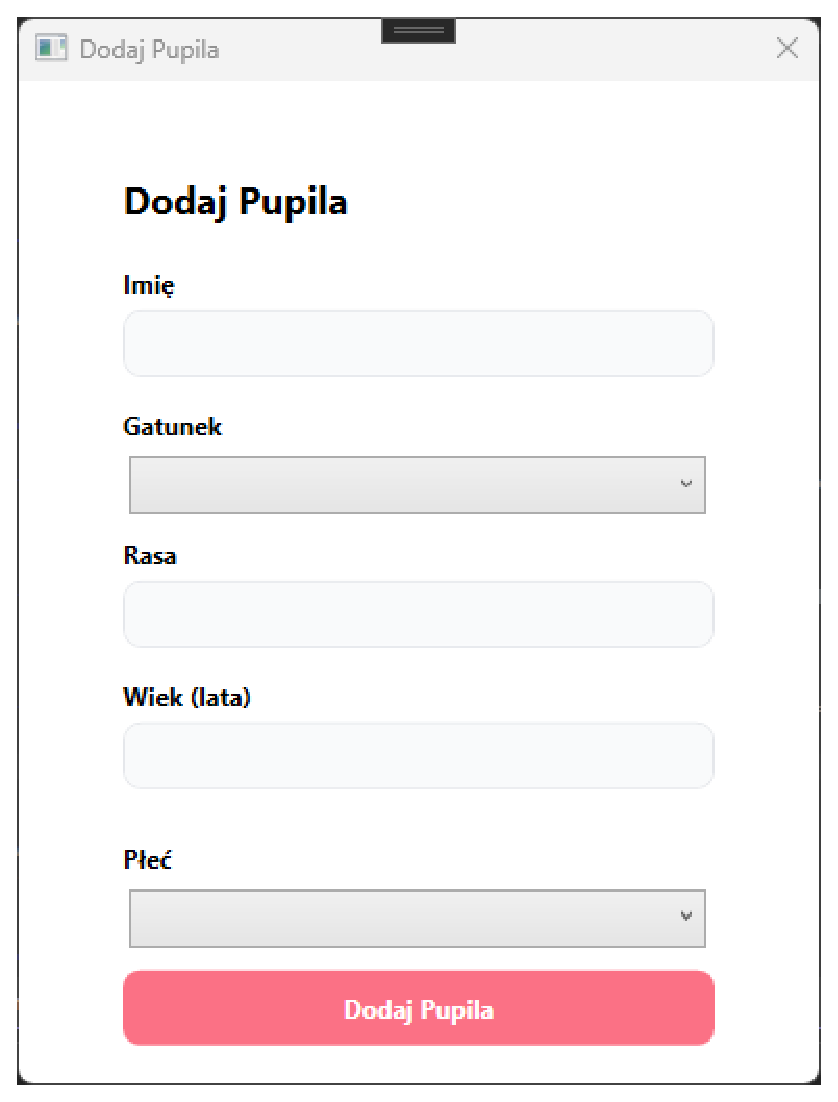
\includegraphics[width=0.7\linewidth]{figures/Uzytkownik/fig_024.eps}
\caption{Widok okna Dodaj pupila.\label{fig24}}
\end{figure}

W przypadku gdy użytkownik nie wypełni wszystkich pól formularza, aplikacja wyświetla komunikat błędu informujący o konieczności uzupełnienia wszystkich pól.

\begin{figure}[H]
\centering
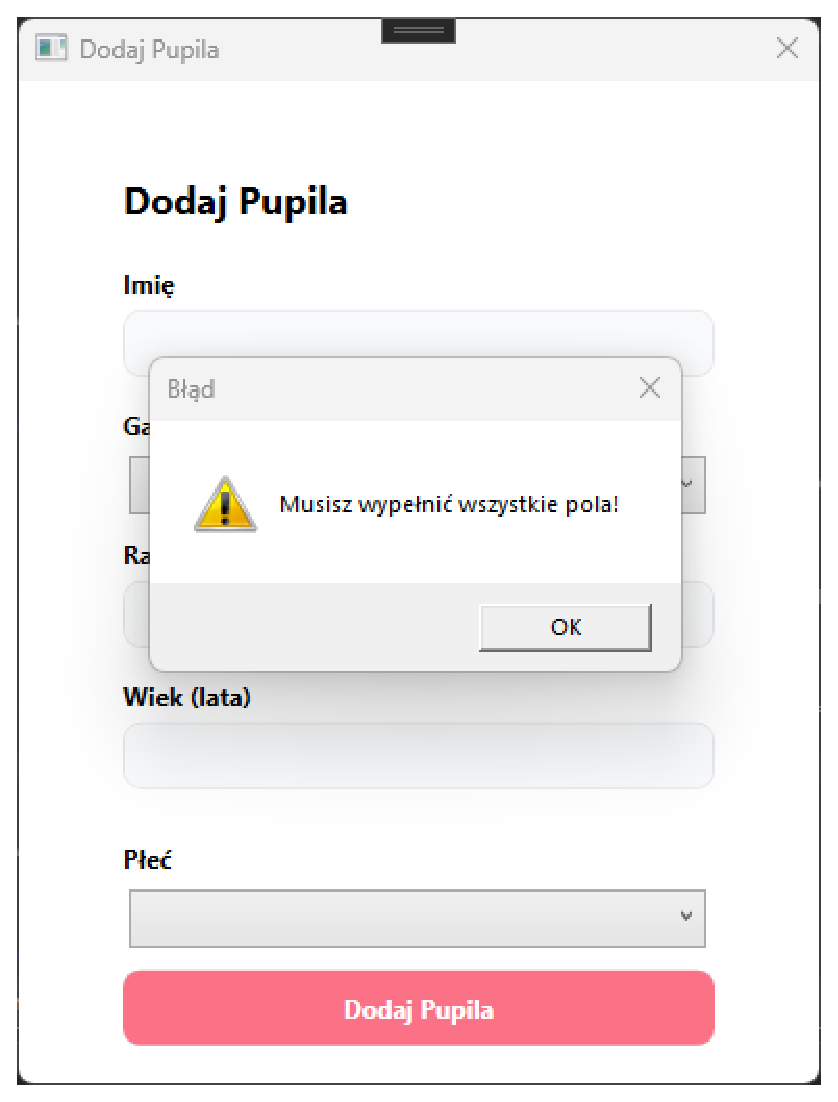
\includegraphics[width=0.7\linewidth]{figures/Uzytkownik/fig_025.eps}
\caption{Komunikat błędu przy niewypełnionych polach formularza.\label{fig25}}
\end{figure}

Po poprawnym wypełnieniu wszystkich pól i kliknięciu przycisku Dodaj Pupila nowy pupil zostaje zapisany w bazie danych i 
przypisany do zalogowanego użytkownika. Aplikacja wyświetla komunikat potwierdzający pomyślne dodanie pupila, a okno zostaje zamknięte.

\begin{figure}[H]
\centering
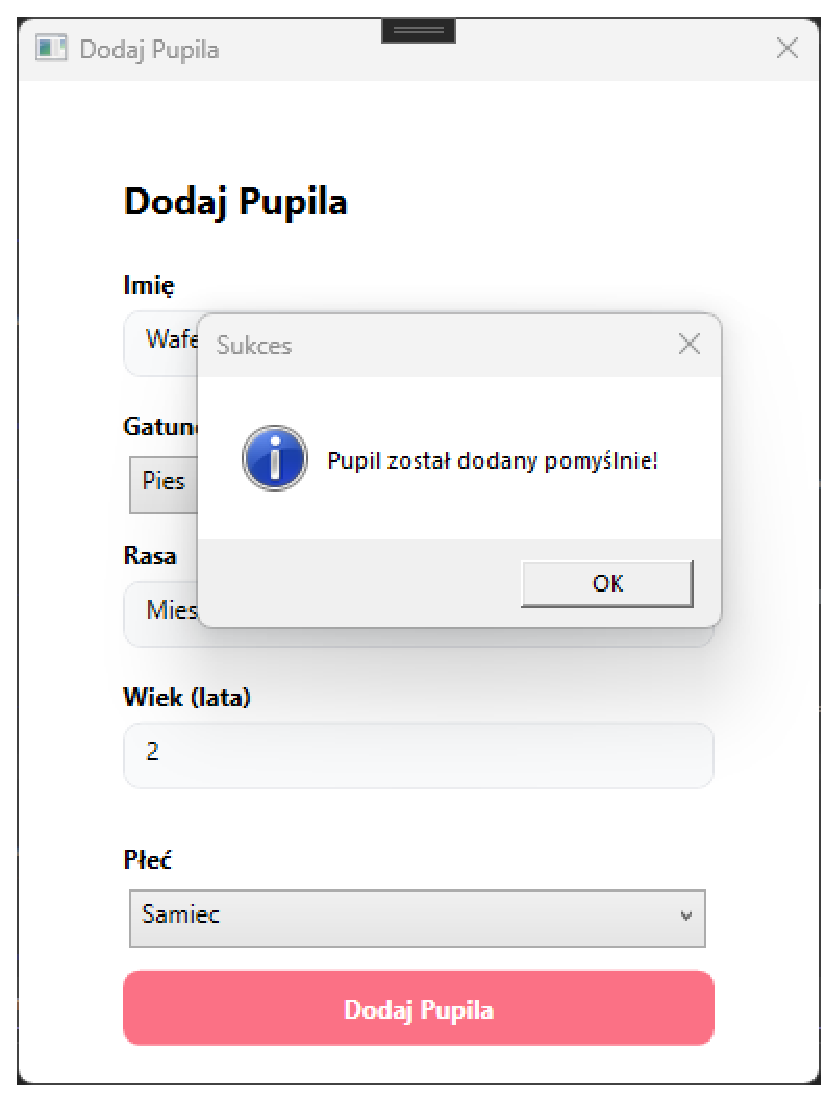
\includegraphics[width=0.7\linewidth]{figures/Uzytkownik/fig_026.eps}
\caption{Komunikat potwierdzający pomyślne dodanie pupila.\label{fig26}}
\end{figure}

\textbf{Okno "Nowa rezerwacja"}

Okno "Nowa rezerwacja" otwierane jest po kliknięciu przycisku Zarezerwuj wizytę w pasku nawigacyjnym. Proces rezerwacji podzielony jest na trzy kroki. 
W pierwszym kroku użytkownik wybiera pupila z listy rozwijanej oraz zabieg z listy dostępnych zabiegów. Dla każdego zabiegu wyświetlany jest czas trwania oraz cena.

\begin{figure}[H]
\centering
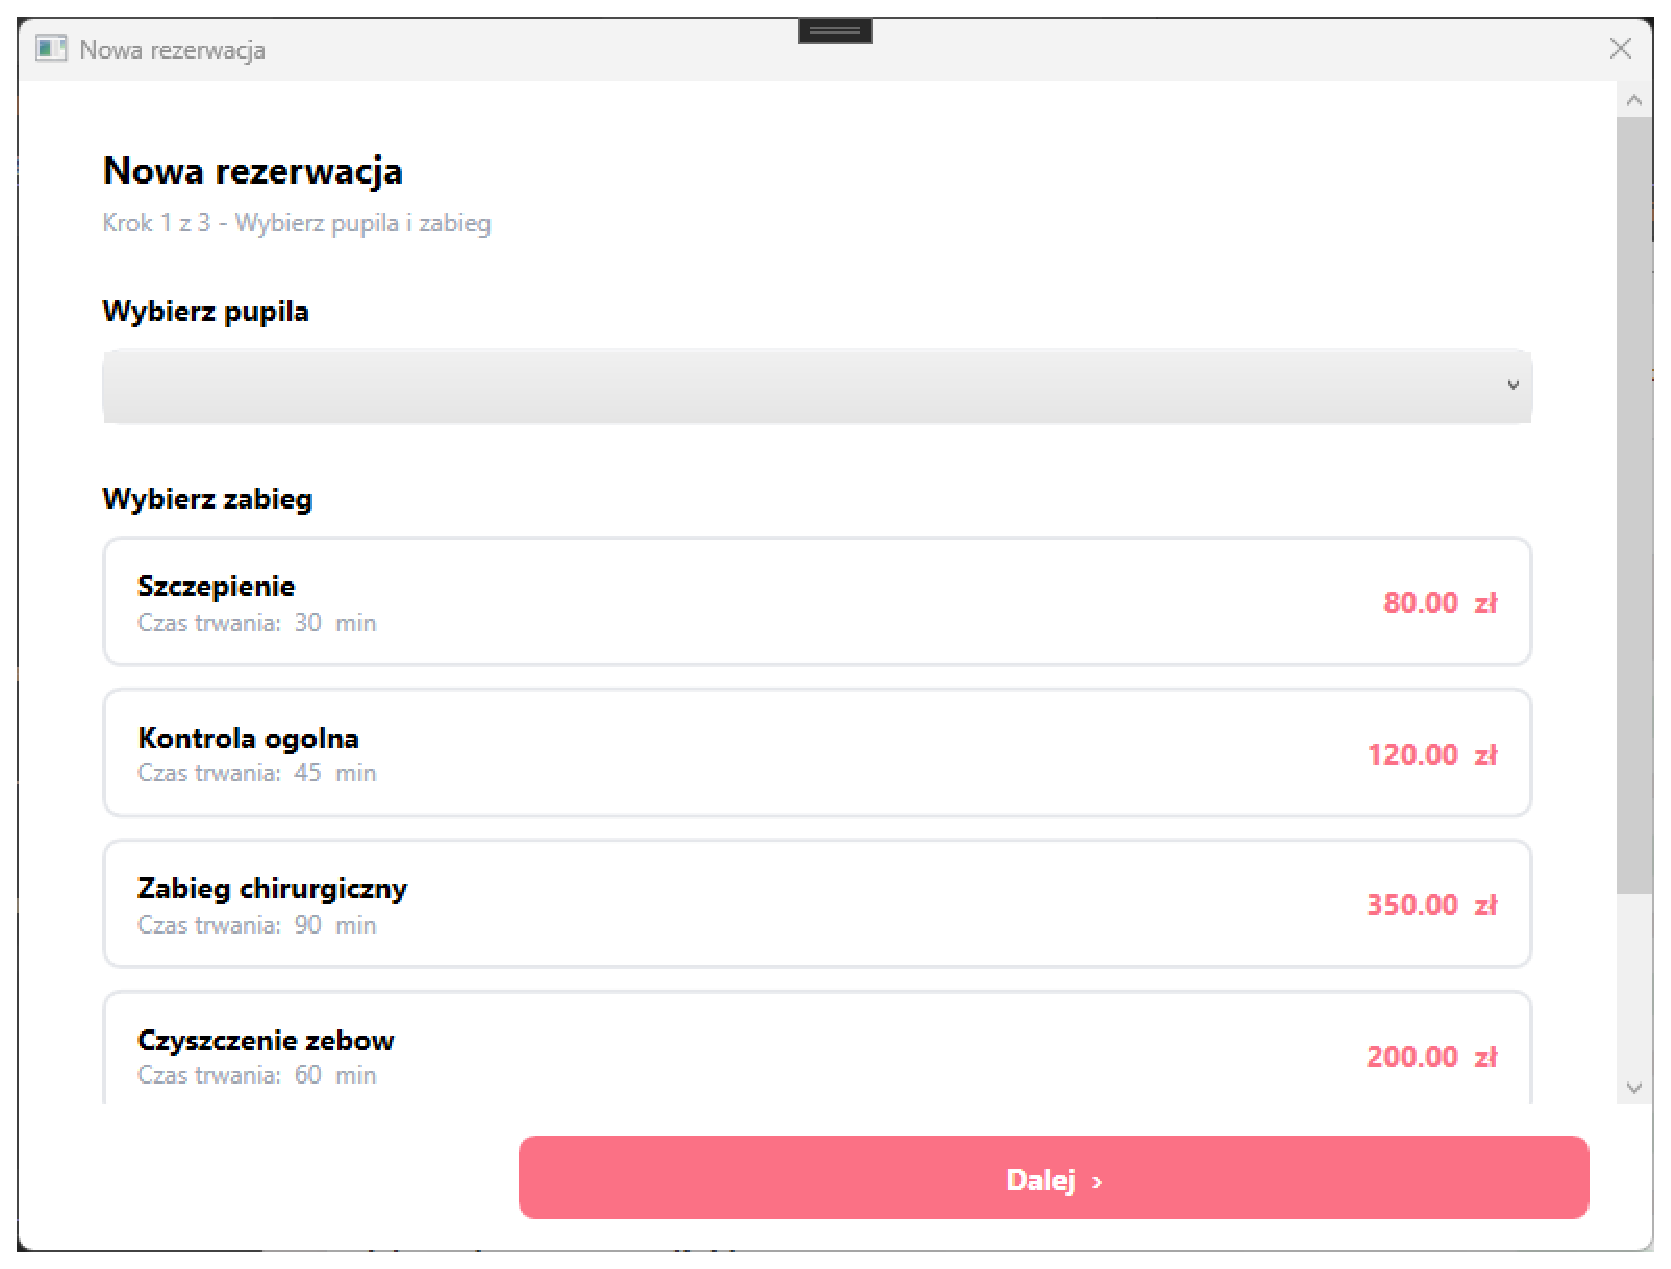
\includegraphics[width=0.9\linewidth]{figures/Uzytkownik/fig_027.eps}
\caption{Krok 1 - widok wyboru pupila i zabiegu.\label{fig27}}
\end{figure}

W przypadku gdy użytkownik nie wybierze pupila przed kliknięciem przycisku Dalej, aplikacja wyświetla komunikat błędu. Analogicznie, jeśli 
użytkownik nie wybierze zabiegu, wyświetlany jest odpowiedni komunikat.

\begin{figure}[H]
\centering
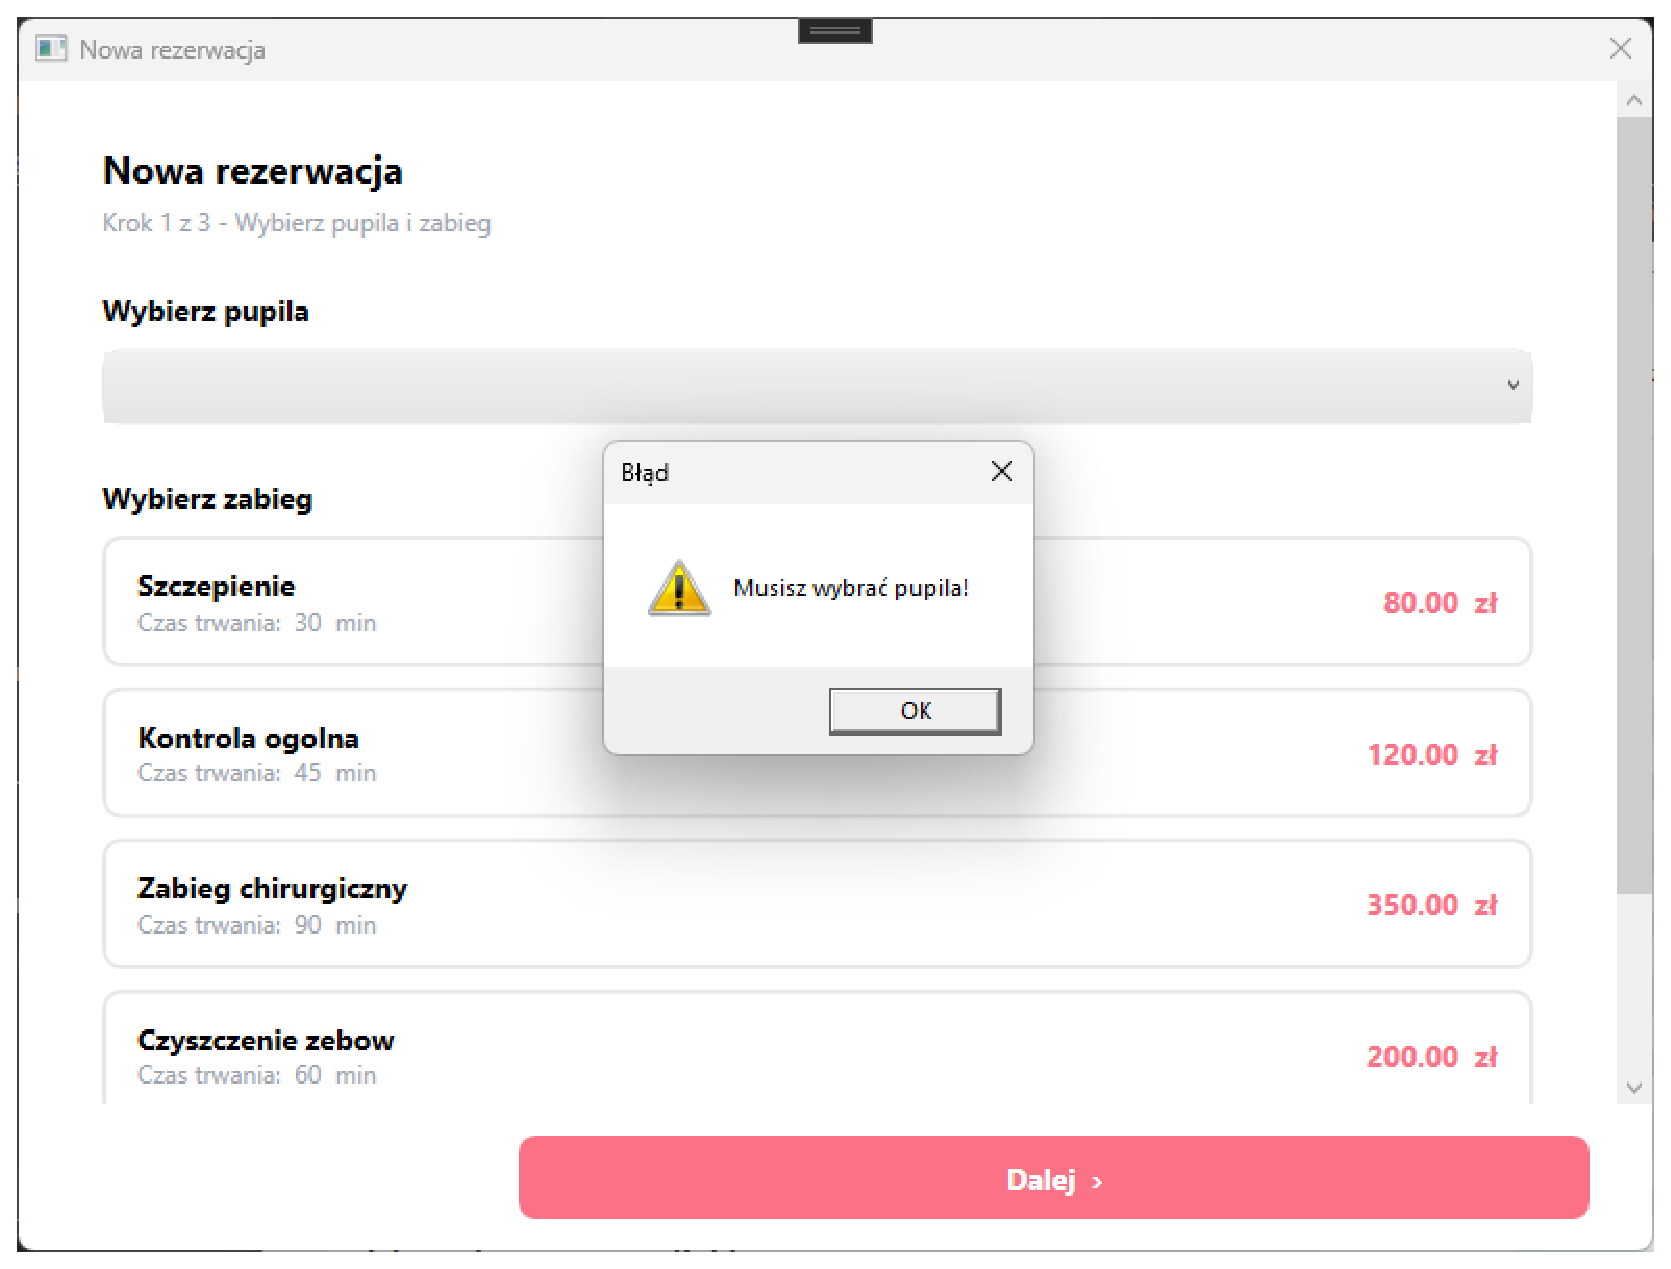
\includegraphics[width=0.9\linewidth]{figures/Uzytkownik/fig_028.eps}
\caption{Komunikat błędu przy braku wybranego pupila.\label{fig28}}
\end{figure}

\begin{figure}[H]
\centering
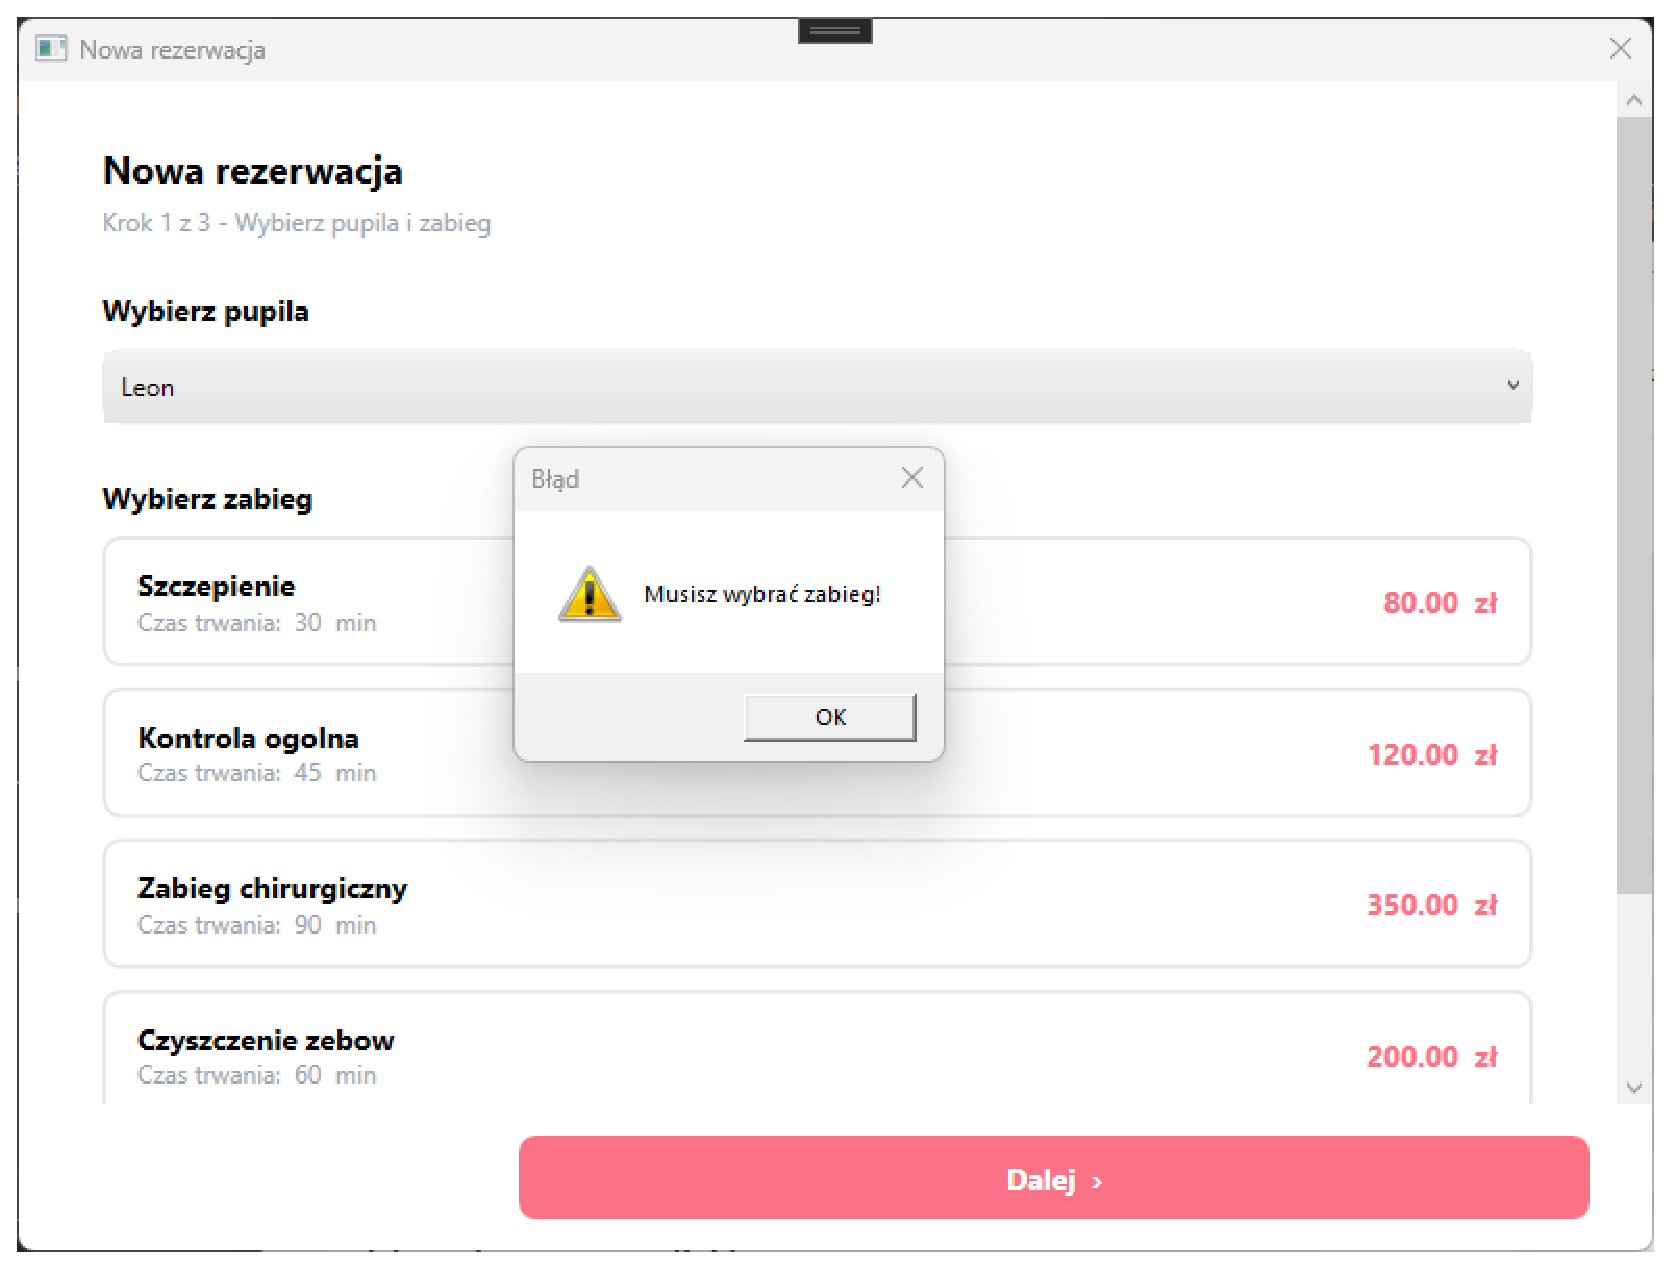
\includegraphics[width=0.9\linewidth]{figures/Uzytkownik/fig_029.eps}
\caption{Komunikat błędu przy braku wybranego zabiegu.\label{fig29}}
\end{figure}

W drugim kroku użytkownik wybiera weterynarza spośród tych, którzy wykonują wybrany zabieg. 
Dla każdego weterynarza wyświetlane jest imię, nazwisko oraz specjalizacja.

\begin{figure}[H]
\centering
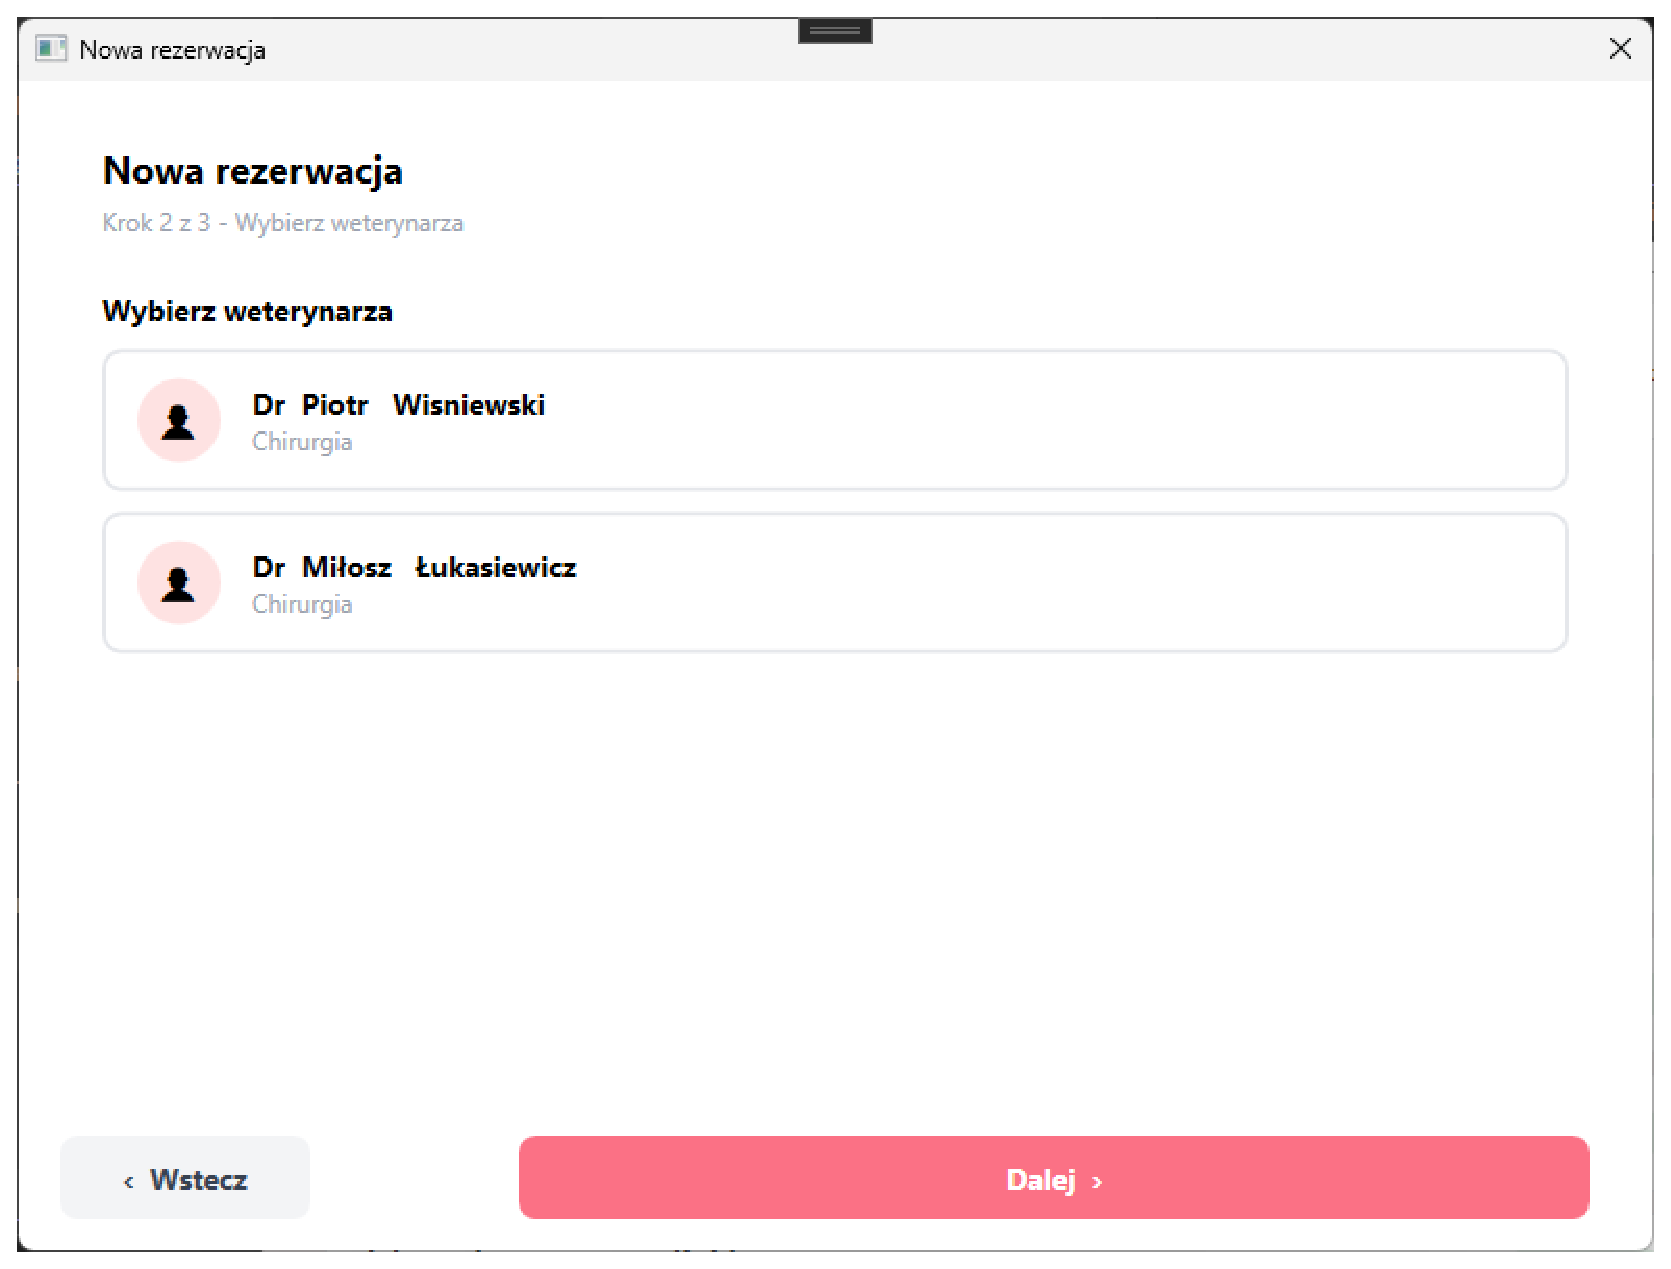
\includegraphics[width=0.9\linewidth]{figures/Uzytkownik/fig_030.eps}
\caption{Krok 2 - widok wyboru weterynarza.\label{fig30}}
\end{figure}

W przypadku gdy użytkownik nie wybierze weterynarza przed kliknięciem przycisku Dalej, aplikacja wyświetla komunikat błędu.

\begin{figure}[H]
\centering
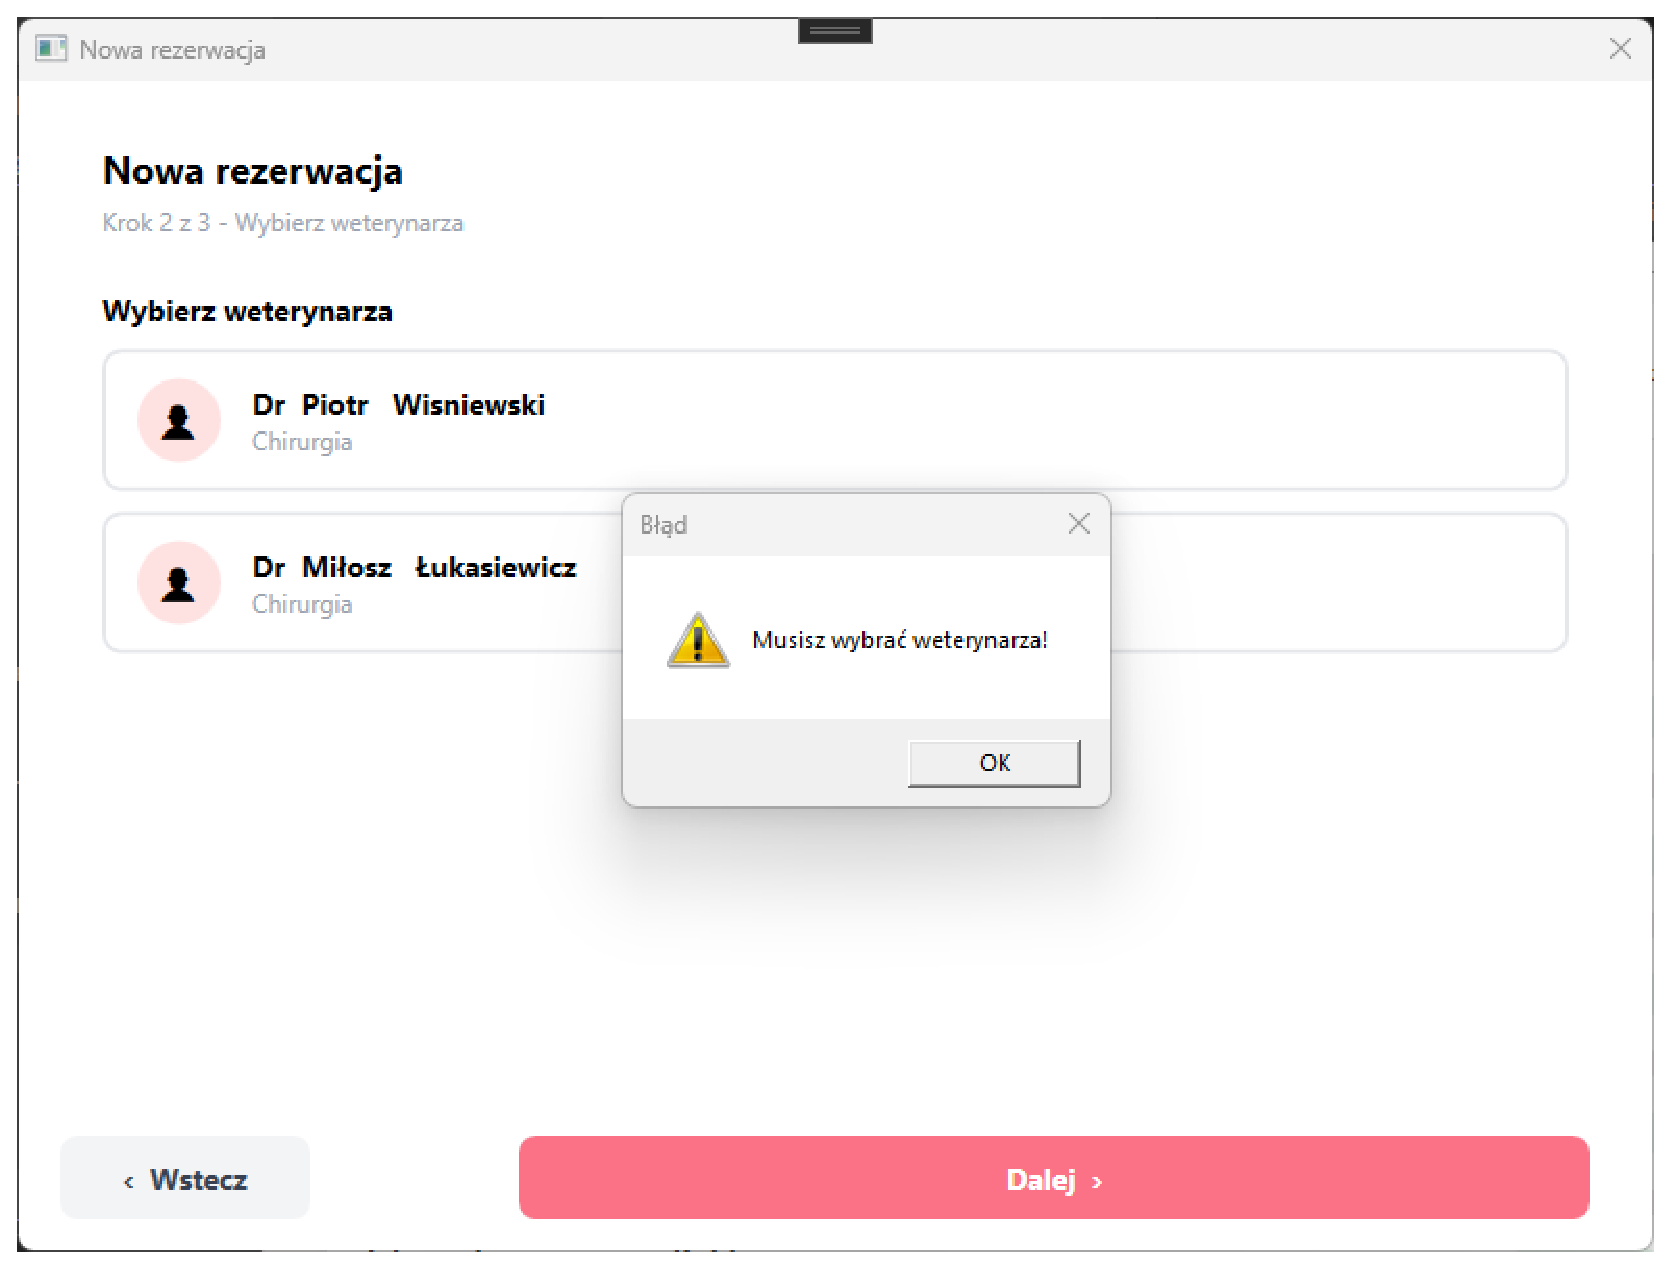
\includegraphics[width=0.9\linewidth]{figures/Uzytkownik/fig_031.eps}
\caption{Komunikat błędu przy braku wybranego weterynarza.\label{fig31}}
\end{figure}

W trzecim kroku użytkownik wybiera termin wizyty z kalendarza dostępności wybranego weterynarza. 
Kalendarz prezentuje tygodniowy widok z podziałem na godziny. Sloty oznaczone kolorem zielonym 
są wolne i możliwe do zarezerwowania, czerwonym zajęte, natomiast szare oznaczają terminy poza 
godzinami pracy weterynarza lub terminy w których zabieg nie zmieści się przed końcem pracy.

\begin{figure}[H]
\centering
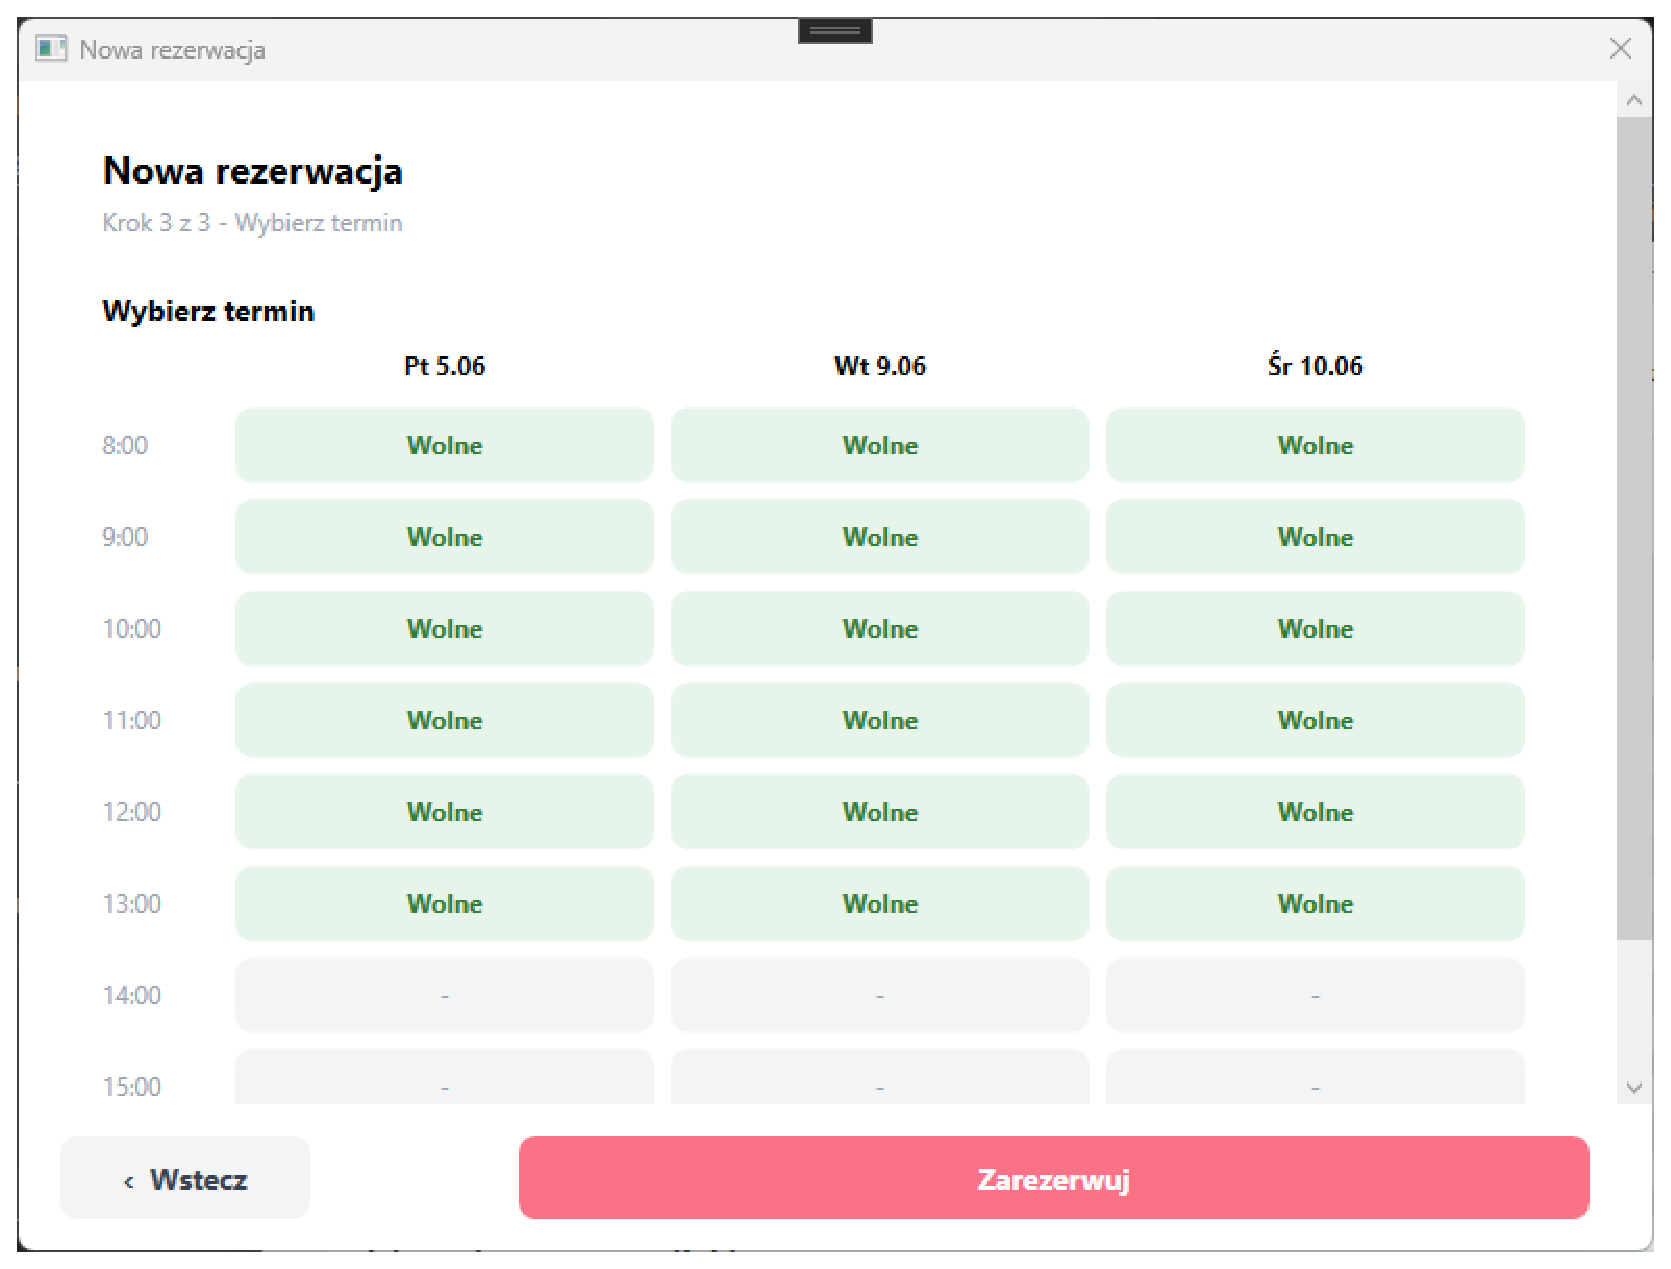
\includegraphics[width=0.9\linewidth]{figures/Uzytkownik/fig_032.eps}
\caption{Krok 3 - widok kalendarza dostępności weterynarza.\label{fig32}}
\end{figure}

W przypadku gdy użytkownik nie wybierze terminu przed kliknięciem przycisku Zarezerwuj, aplikacja wyświetla komunikat błędu.

\begin{figure}[H]
\centering
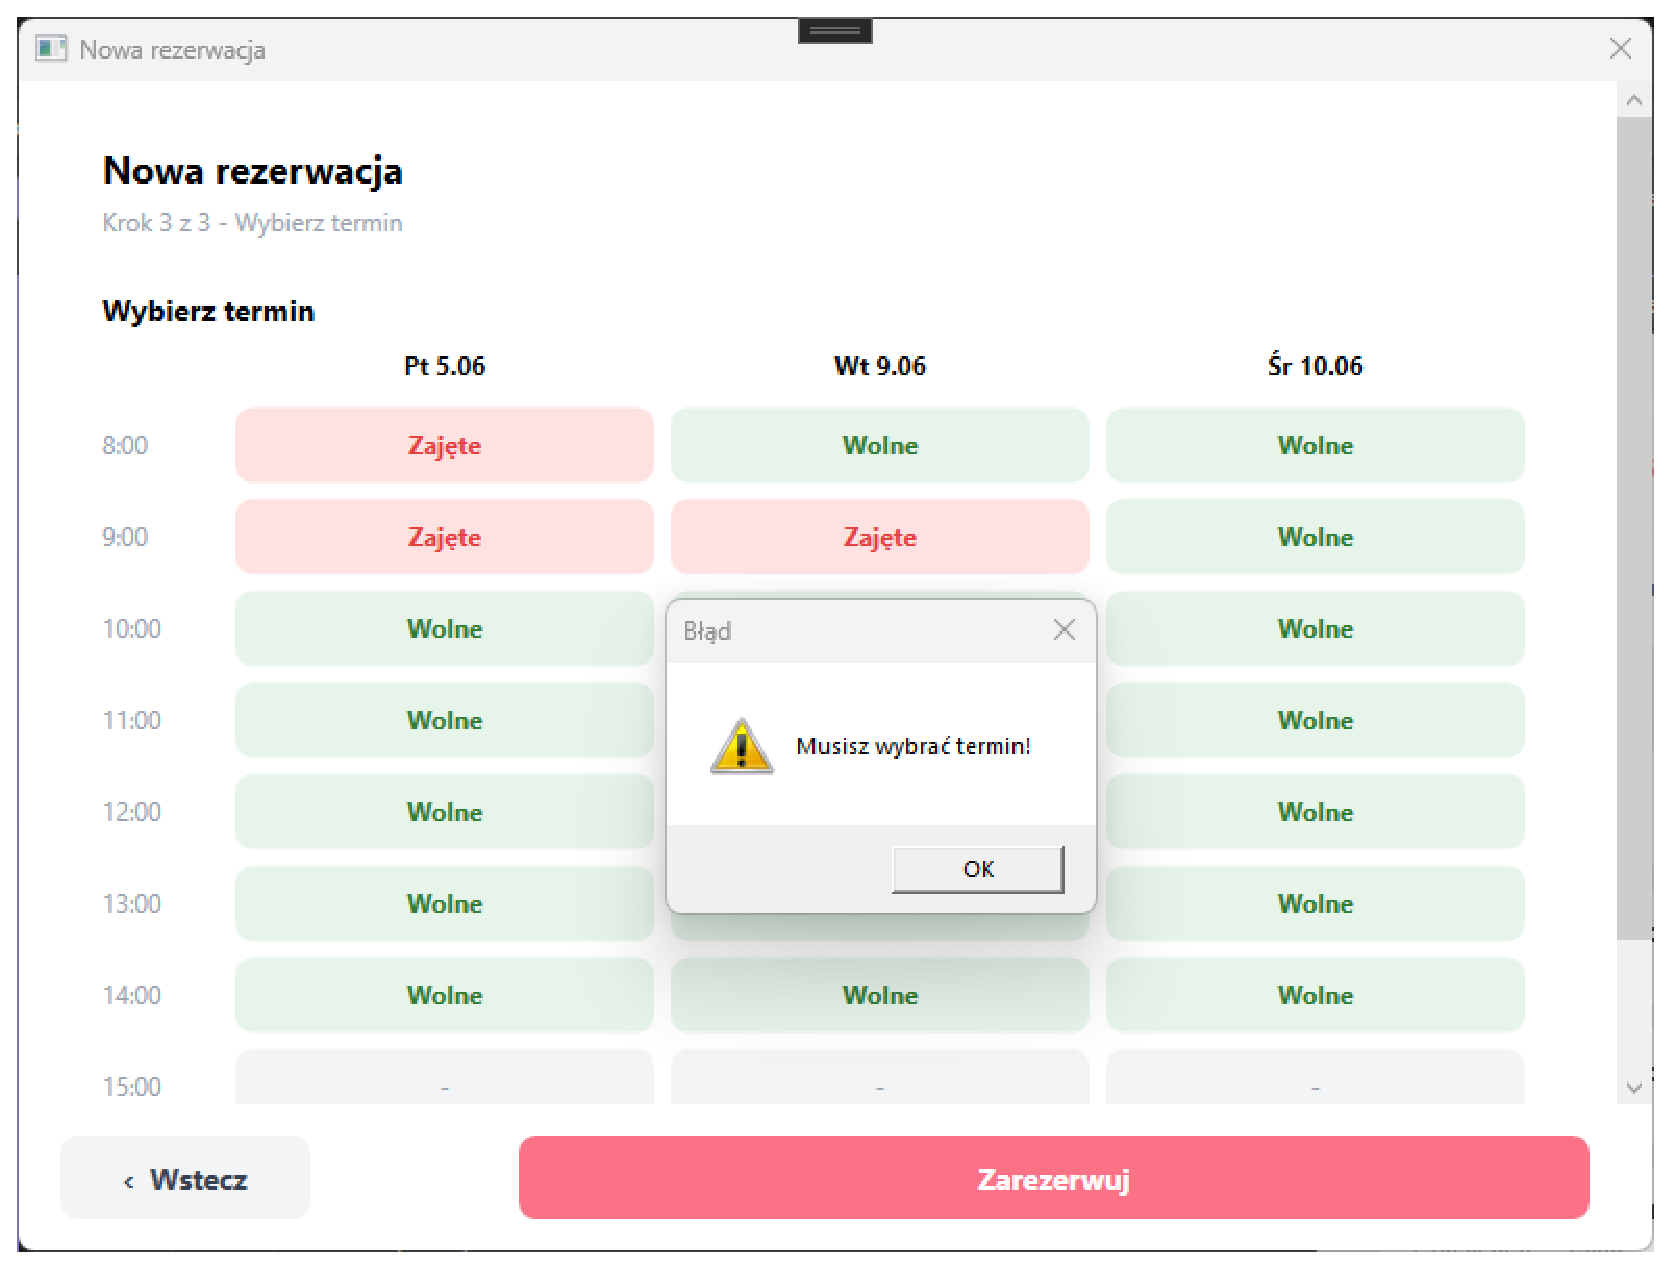
\includegraphics[width=0.9\linewidth]{figures/Uzytkownik/fig_033.eps}
\caption{Komunikat błędu przy braku wybranego terminu.\label{fig33}}
\end{figure}

Po wybraniu wolnego terminu i kliknięciu przycisku Zarezerwuj rezerwacja zostaje zapisana w bazie danych, a z 
konta użytkownika pobierana jest kwota odpowiadająca cenie zabiegu. Aplikacja wyświetla komunikat potwierdzający 
pomyślne zapisanie rezerwacji wraz z informacją o pobranej kwocie oraz pozostałym saldzie.

\begin{figure}[H]
\centering
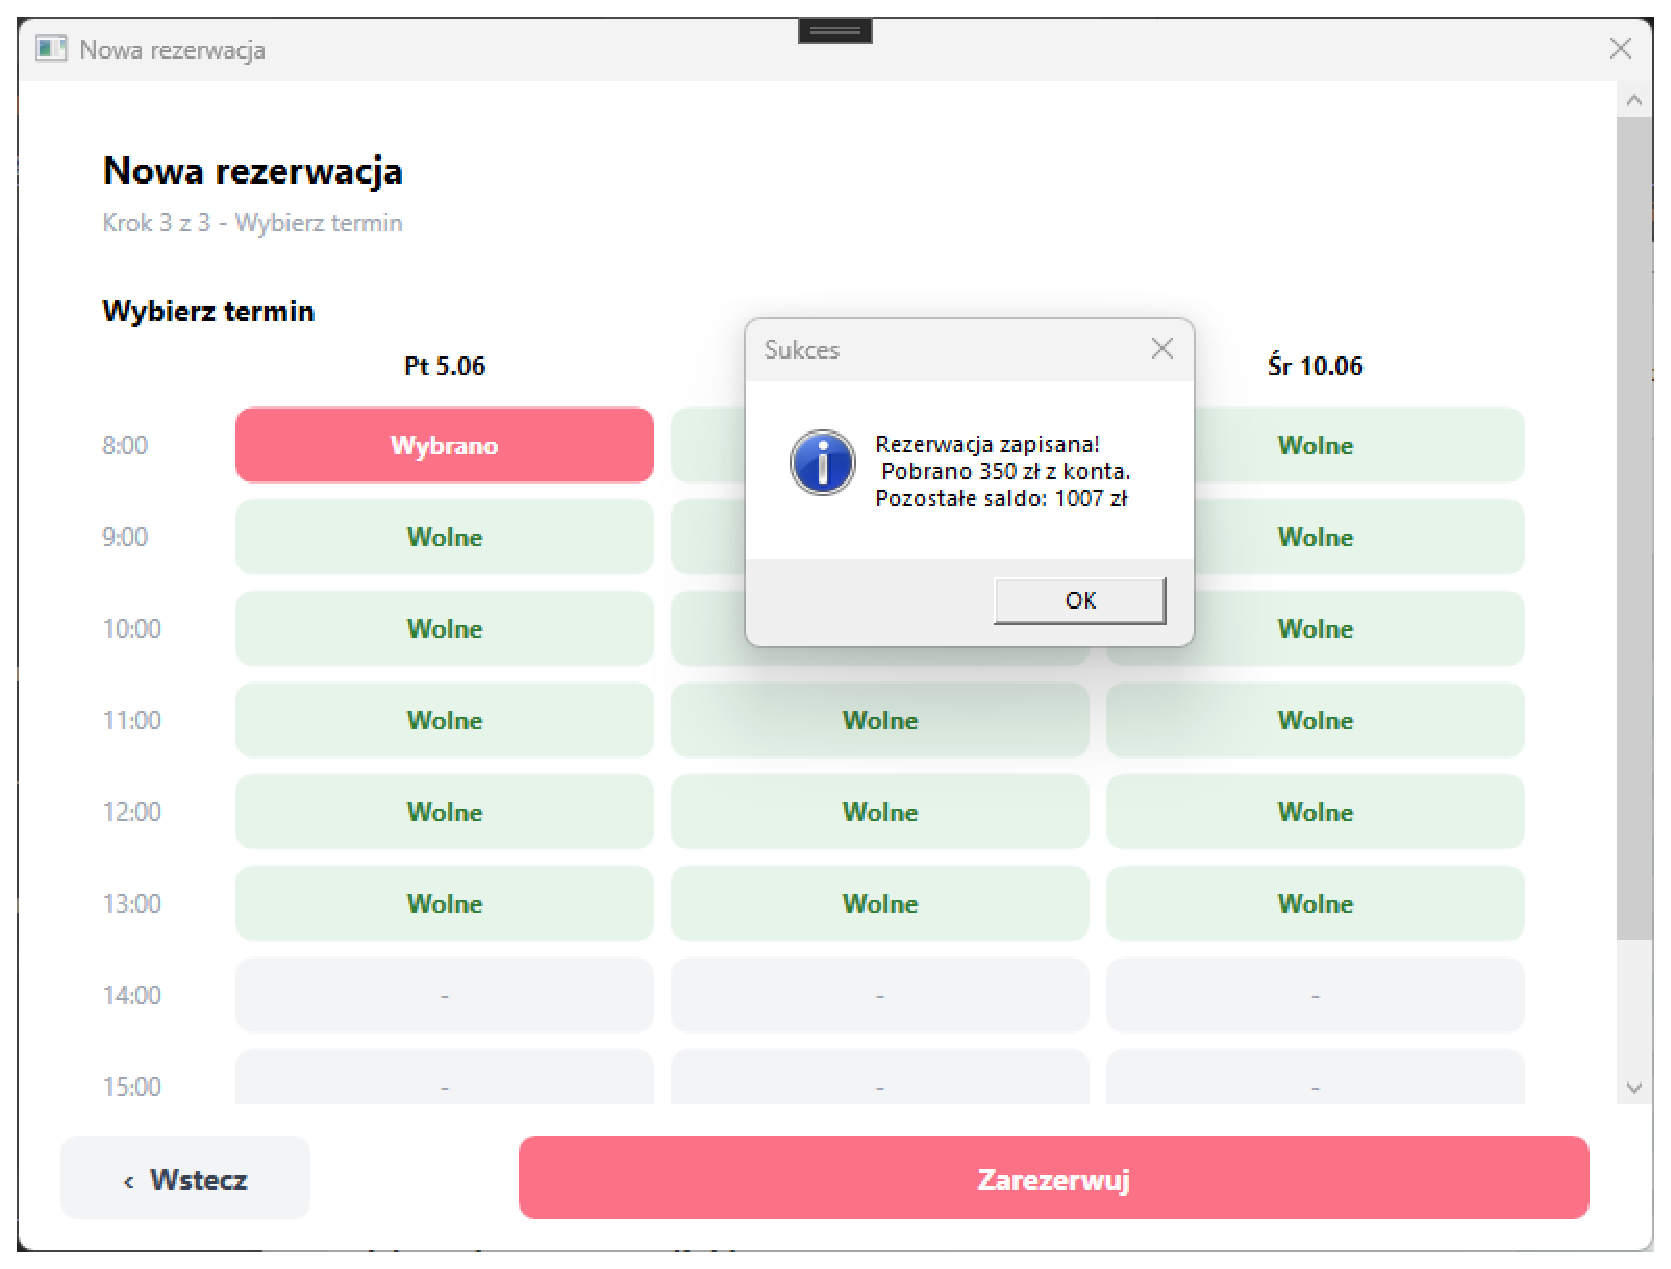
\includegraphics[width=0.9\linewidth]{figures/Uzytkownik/fig_034.eps}
\caption{Komunikat potwierdzający pomyślne zapisanie rezerwacji.\label{fig34}}
\end{figure}

\textbf{Zakładka "Dodaj środki"}

Zakładka "Dodaj środki" umożliwia użytkownikowi doładowanie salda swojego konta. Formularz zawiera jedno pole tekstowe 
do wprowadzenia kwoty wpłaty oraz przycisk Wpłać. Aktualne saldo konta wyświetlane jest na bieżąco w górnym pasku aplikacji.

\begin{figure}[H]
\centering
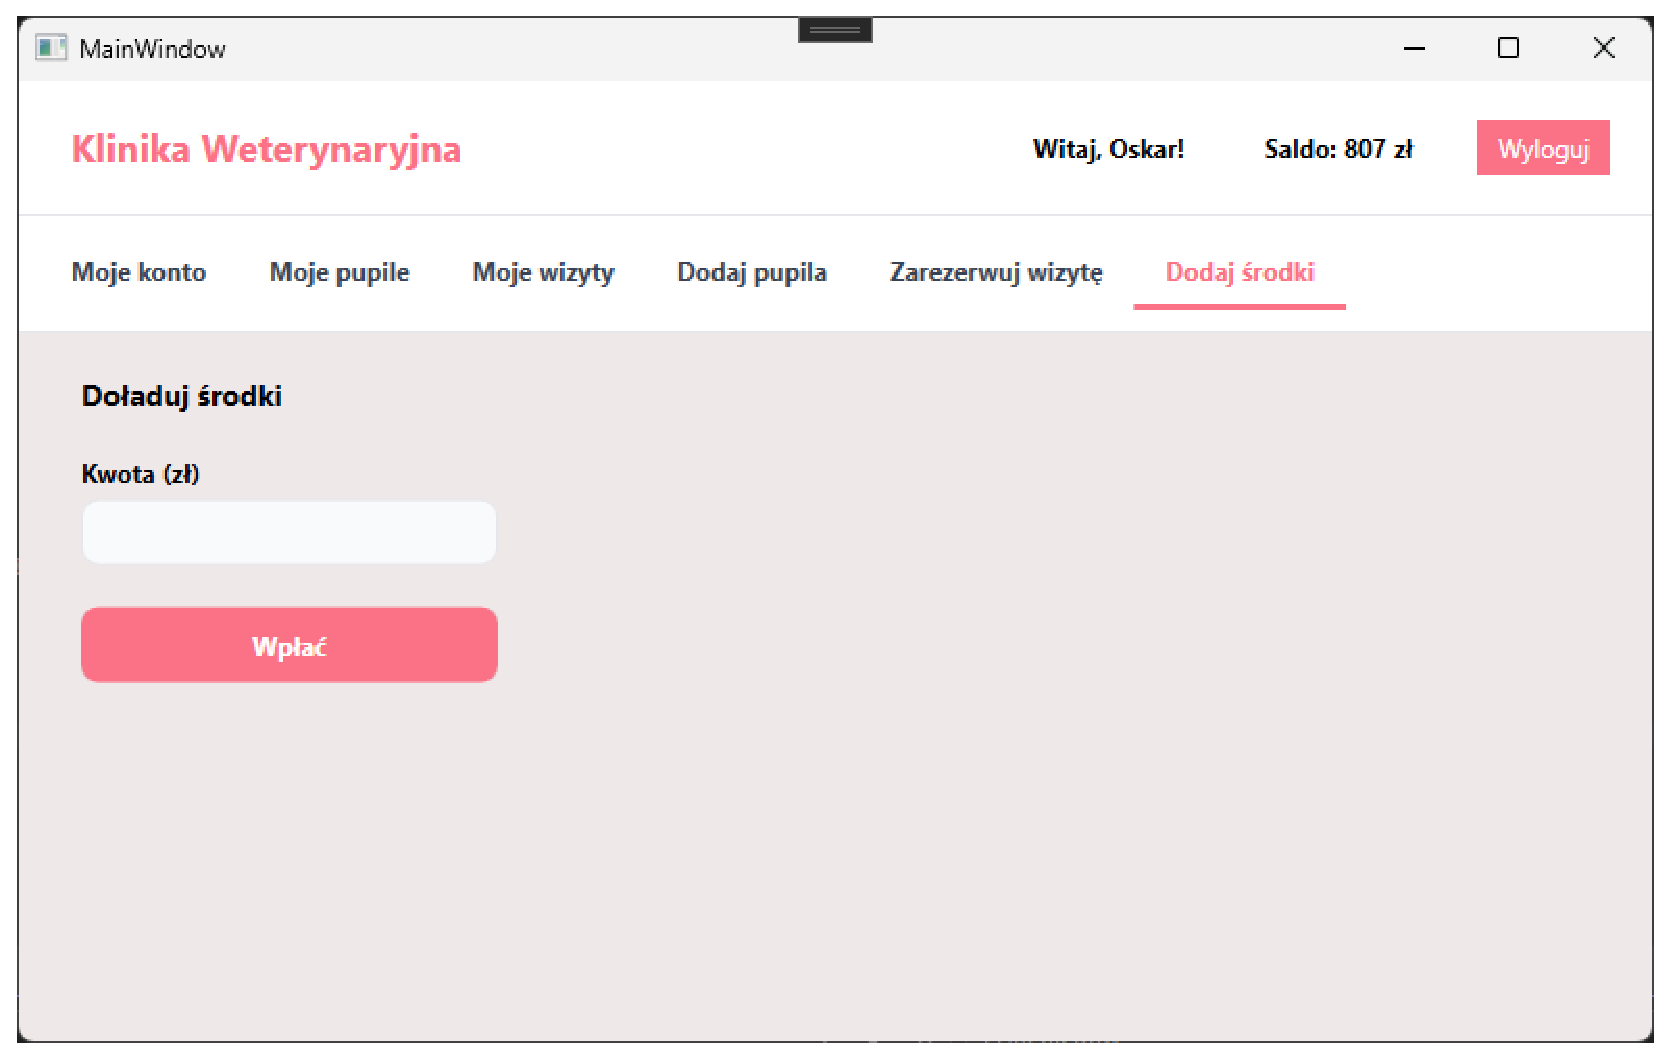
\includegraphics[width=0.9\linewidth]{figures/Uzytkownik/fig_035.eps}
\caption{Widok zakładki Dodaj środki.\label{fig35}}
\end{figure}

W przypadku gdy użytkownik nie wprowadzi żadnej kwoty i kliknie przycisk Wpłać, aplikacja wyświetla komunikat 
błędu informujący o konieczności podania prawidłowej kwoty.

\begin{figure}[H]
\centering
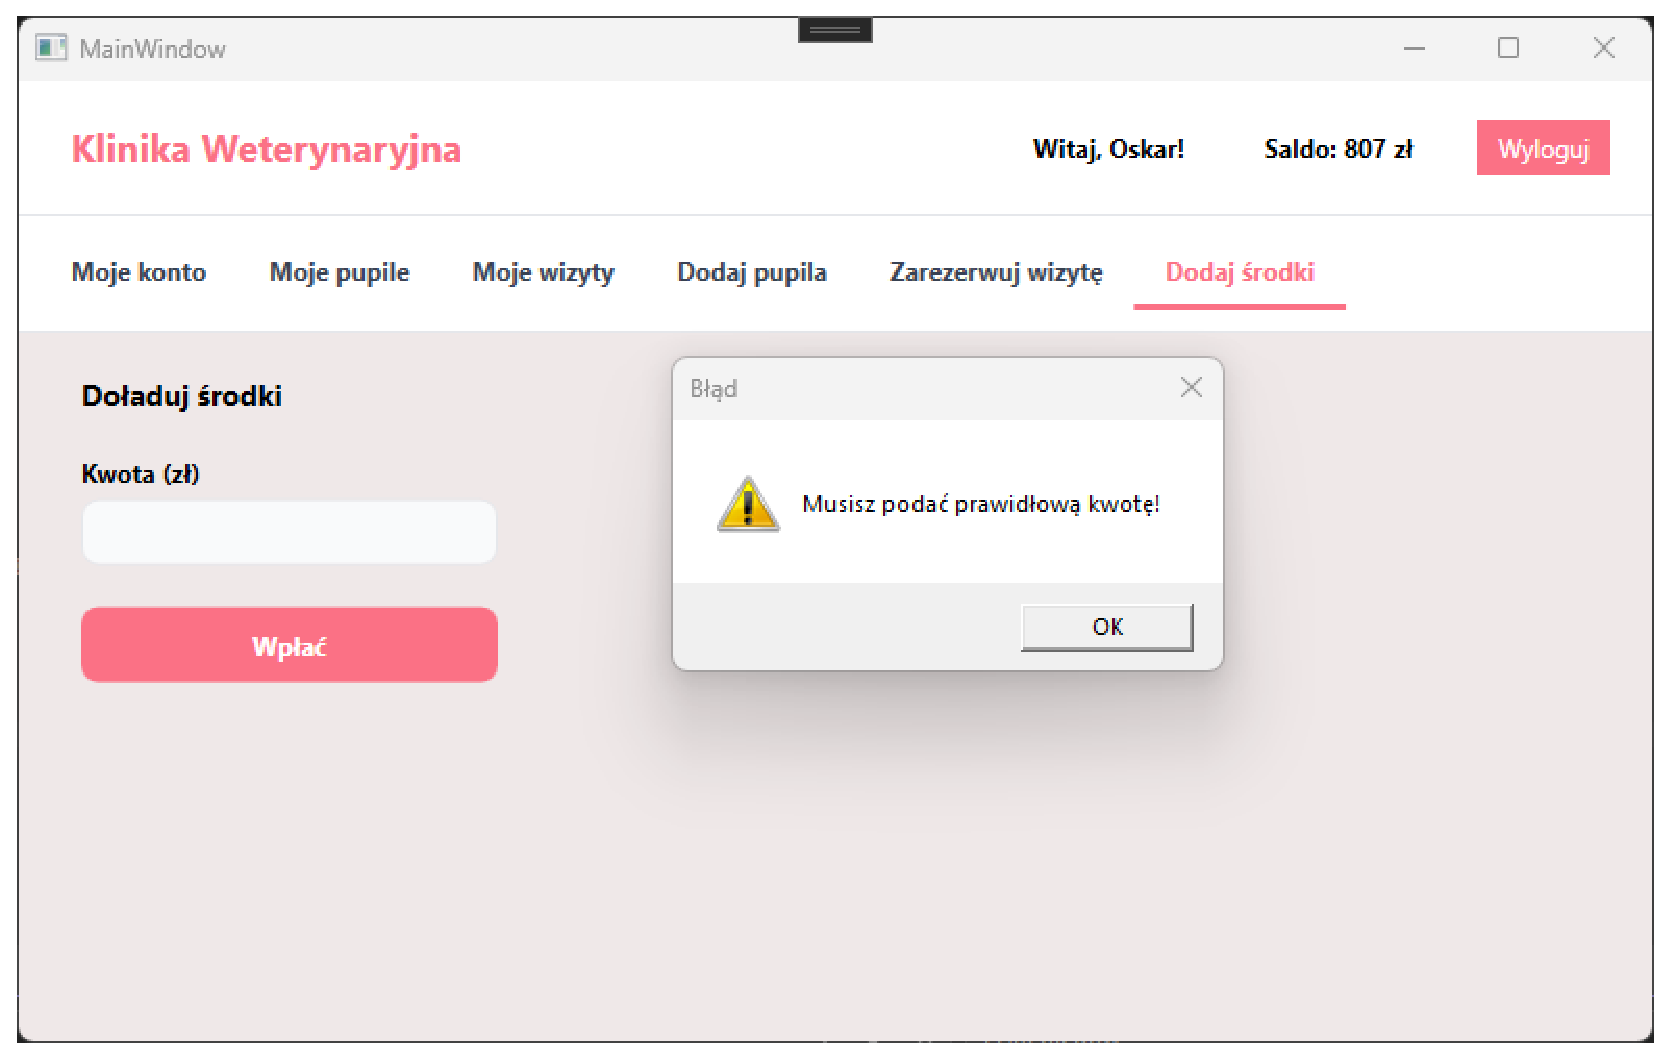
\includegraphics[width=0.9\linewidth]{figures/Uzytkownik/fig_036.eps}
\caption{Komunikat błędu przy pustym polu kwoty.\label{fig36}}
\end{figure}

Aplikacja waliduje również podaną kwotę - nie może ona być liczbą ujemną ani równą zero. 
W przypadku podania nieprawidłowej wartości wyświetlany jest komunikat błędu.

\begin{figure}[H]
\centering
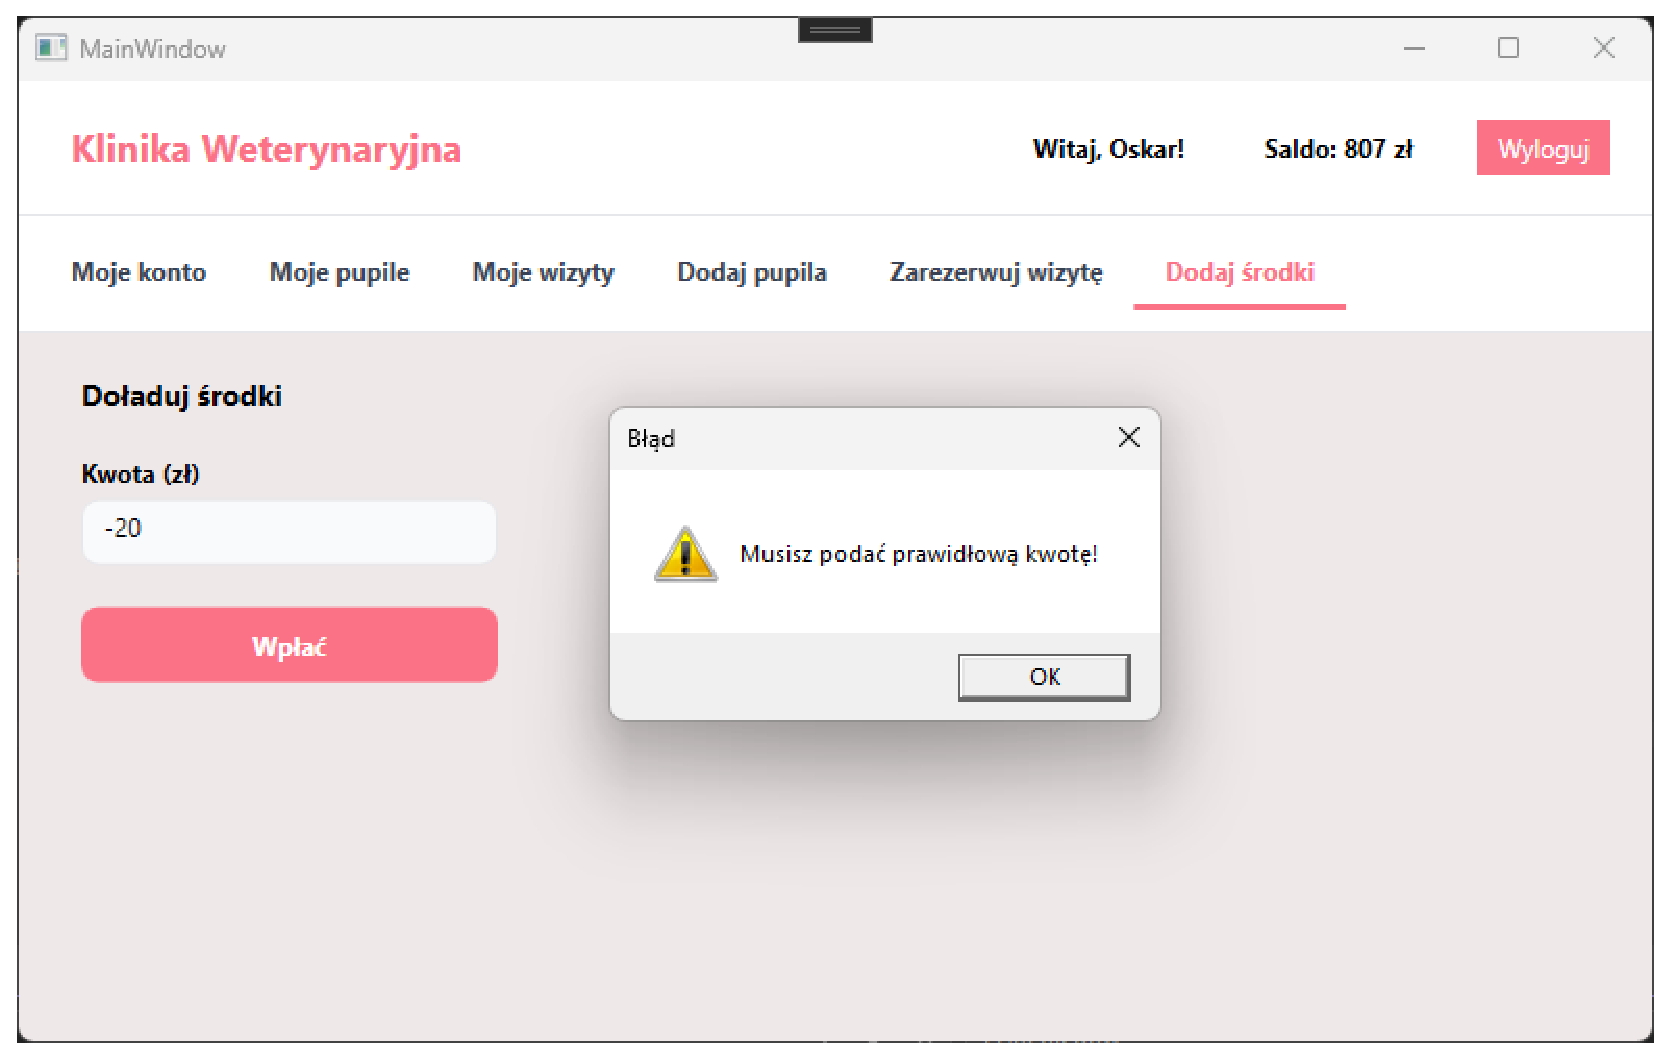
\includegraphics[width=0.9\linewidth]{figures/Uzytkownik/fig_037.eps}
\caption{Komunikat błędu przy podaniu nieprawidłowej kwoty.\label{fig37}}
\end{figure}

Po wprowadzeniu prawidłowej kwoty i kliknięciu przycisku Wpłać aplikacja wyświetla okno dialogowe z prośbą o potwierdzenie 
operacji, informując o kwocie która zostanie dodana do salda.

\begin{figure}[H]
\centering
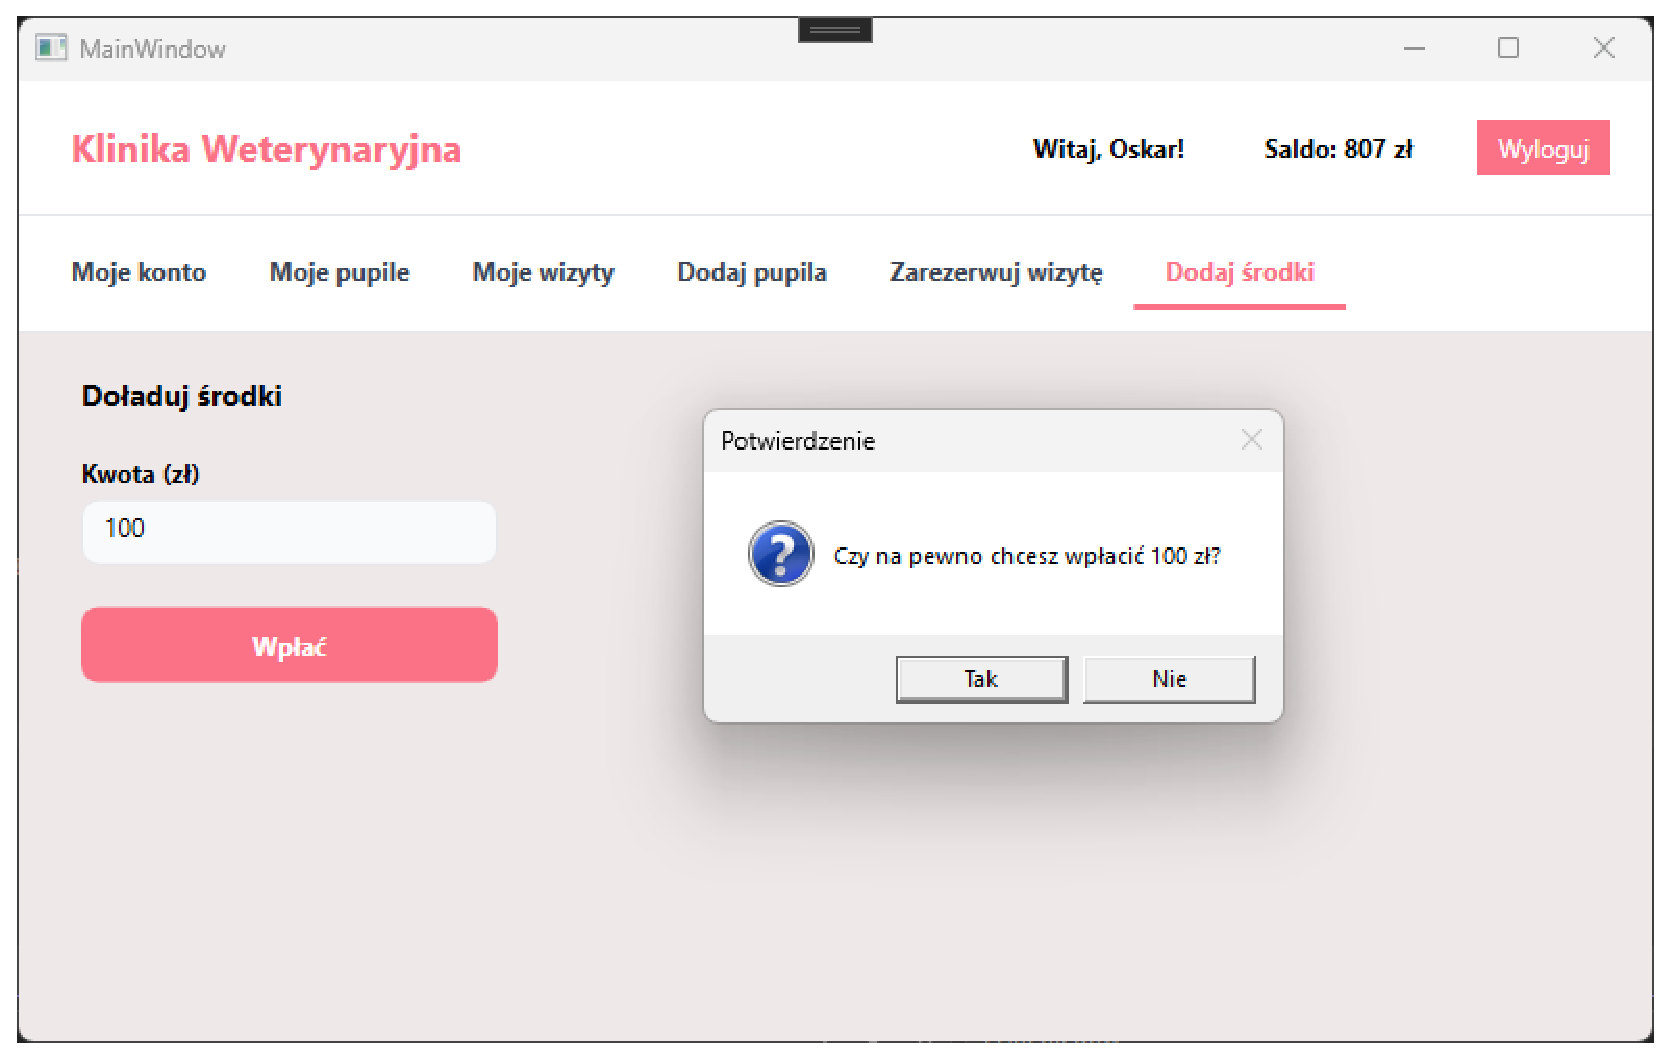
\includegraphics[width=0.9\linewidth]{figures/Uzytkownik/fig_038.eps}
\caption{Okno potwierdzenia wpłaty środków.\label{fig38}}
\end{figure}

Po zatwierdzeniu operacji saldo konta użytkownika zostaje zwiększone o podaną kwotę, zarówno w bazie 
danych jak i w interfejsie aplikacji. Aplikacja wyświetla komunikat potwierdzający pomyślne wykonanie 
wpłaty, a pole tekstowe zostaje wyczyszczone.

\begin{figure}[H]
\centering
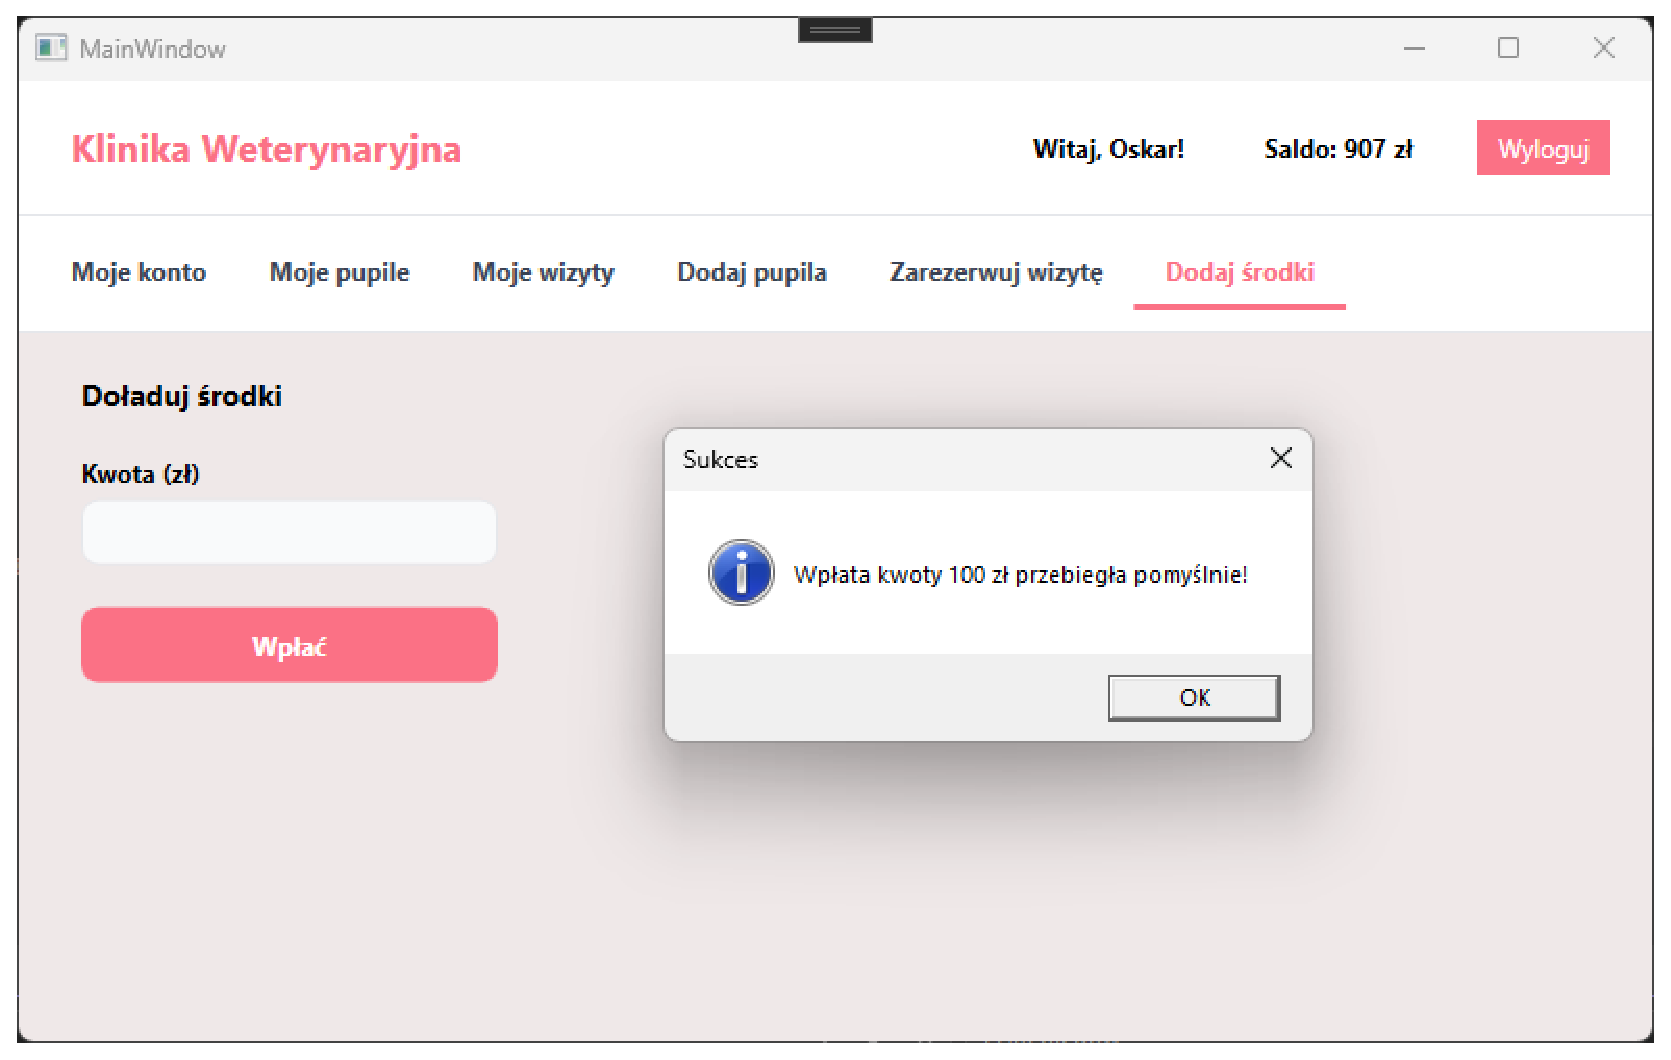
\includegraphics[width=0.9\linewidth]{figures/Uzytkownik/fig_039.eps}
\caption{Komunikat potwierdzający pomyślną wpłatę środków.\label{fig39}}
\end{figure}

\section{Panel administratora}

\textbf{Zakładka "Weterynarze"}

Zakładka "Weterynarze" wyświetla listę wszystkich weterynarzy zarejestrowanych w systemie. Dla każdego weterynarza 
prezentowane są informacje takie jak imię, nazwisko, specjalizacja, adres e-mail oraz numer telefonu. 
Przy każdym weterynarzu dostępne są dwa przyciski akcji: + umożliwiający zarządzanie zabiegami przypisanymi do weterynarza oraz X umożliwiający 
usunięcie weterynarza z systemu. W prawym górnym rogu zakładki znajduje się przycisk (+ Dodaj weterynarza).

\begin{figure}[H]
\centering
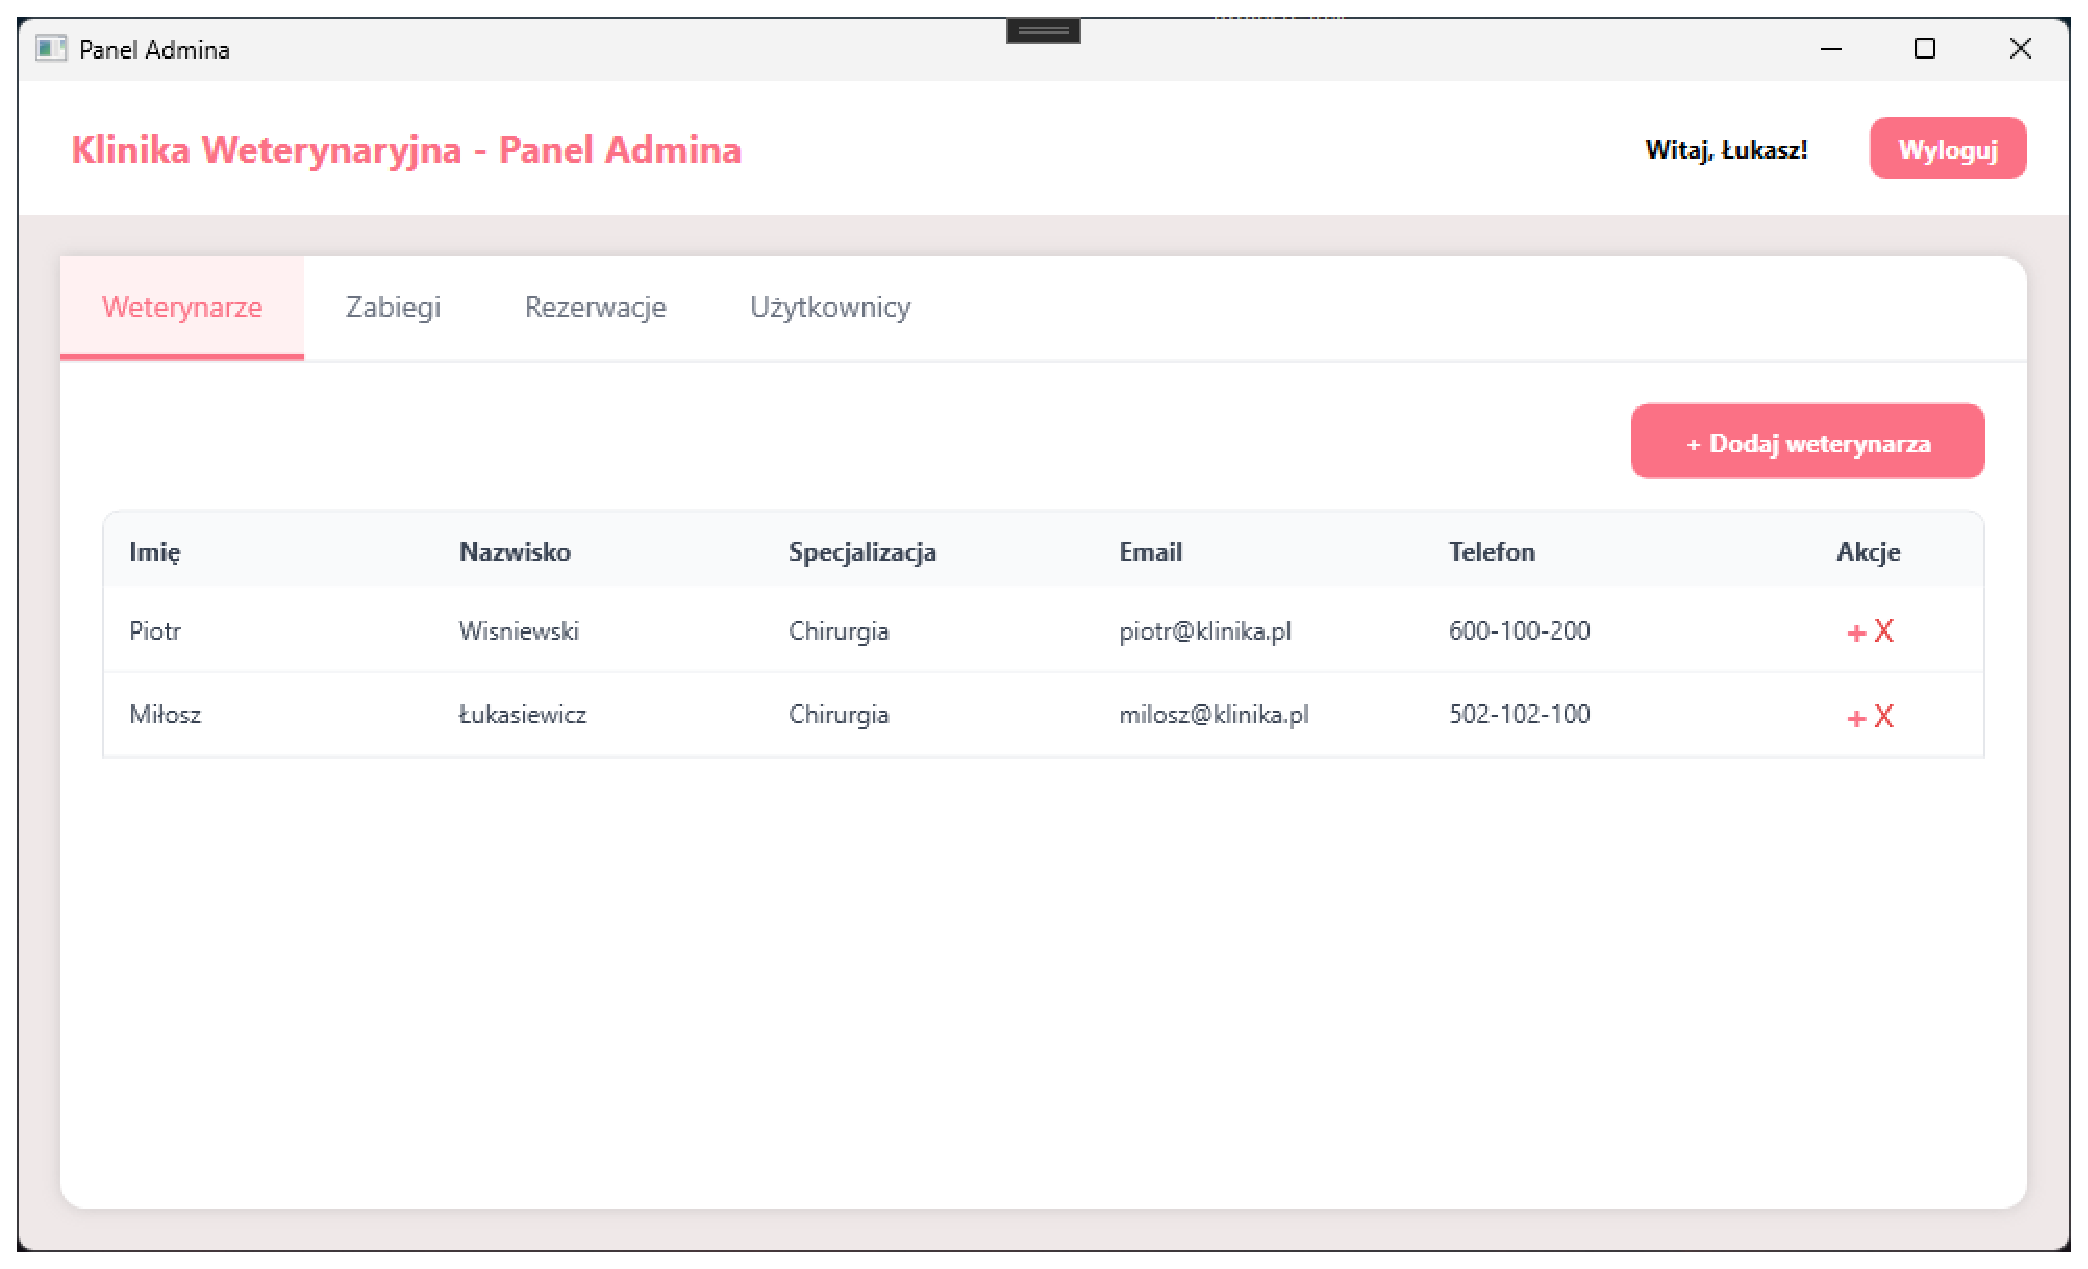
\includegraphics[width=0.9\linewidth]{figures/Admin/fig_040.eps}
\caption{Widok zakładki Weterynarze w panelu administratora.\label{fig40}}
\end{figure}

Po kliknięciu przycisku (+ Dodaj weterynarza) otwierane jest okno formularza. 
Formularz zawiera pola: imię, nazwisko, specjalizacja, email, telefon, hasło oraz sekcję Godziny pracy z polami 
Od i Do dla każdego dnia tygodnia od poniedziałku do piątku. Domyślne godziny pracy ustawione są na 08:00-15:00. Pozostawienie pól 
pustych dla danego dnia oznacza, że weterynarz nie pracuje w tym dniu.

\begin{figure}[H]
\centering
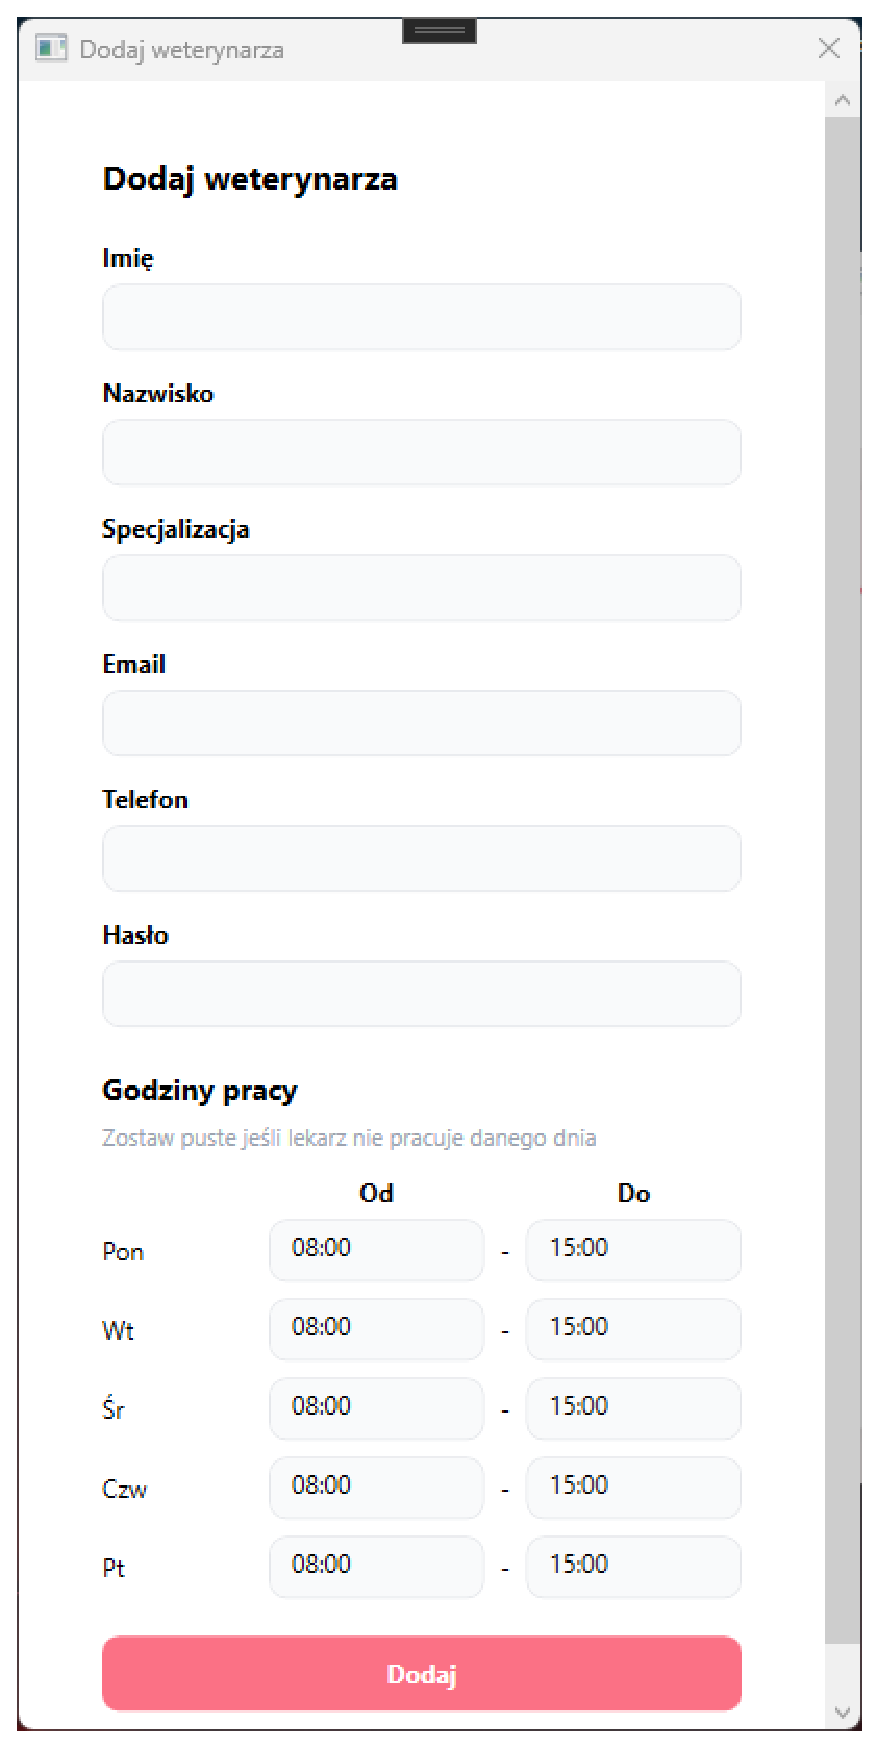
\includegraphics[width=0.6\linewidth]{figures/Admin/fig_041.eps}
\caption{Okno formularza dodawania weterynarza.\label{fig41}}
\end{figure}

W przypadku gdy administrator nie wypełni wymaganych pól (imię, nazwisko, email, hasło) aplikacja wyświetla komunikat błędu.

\begin{figure}[H]
\centering
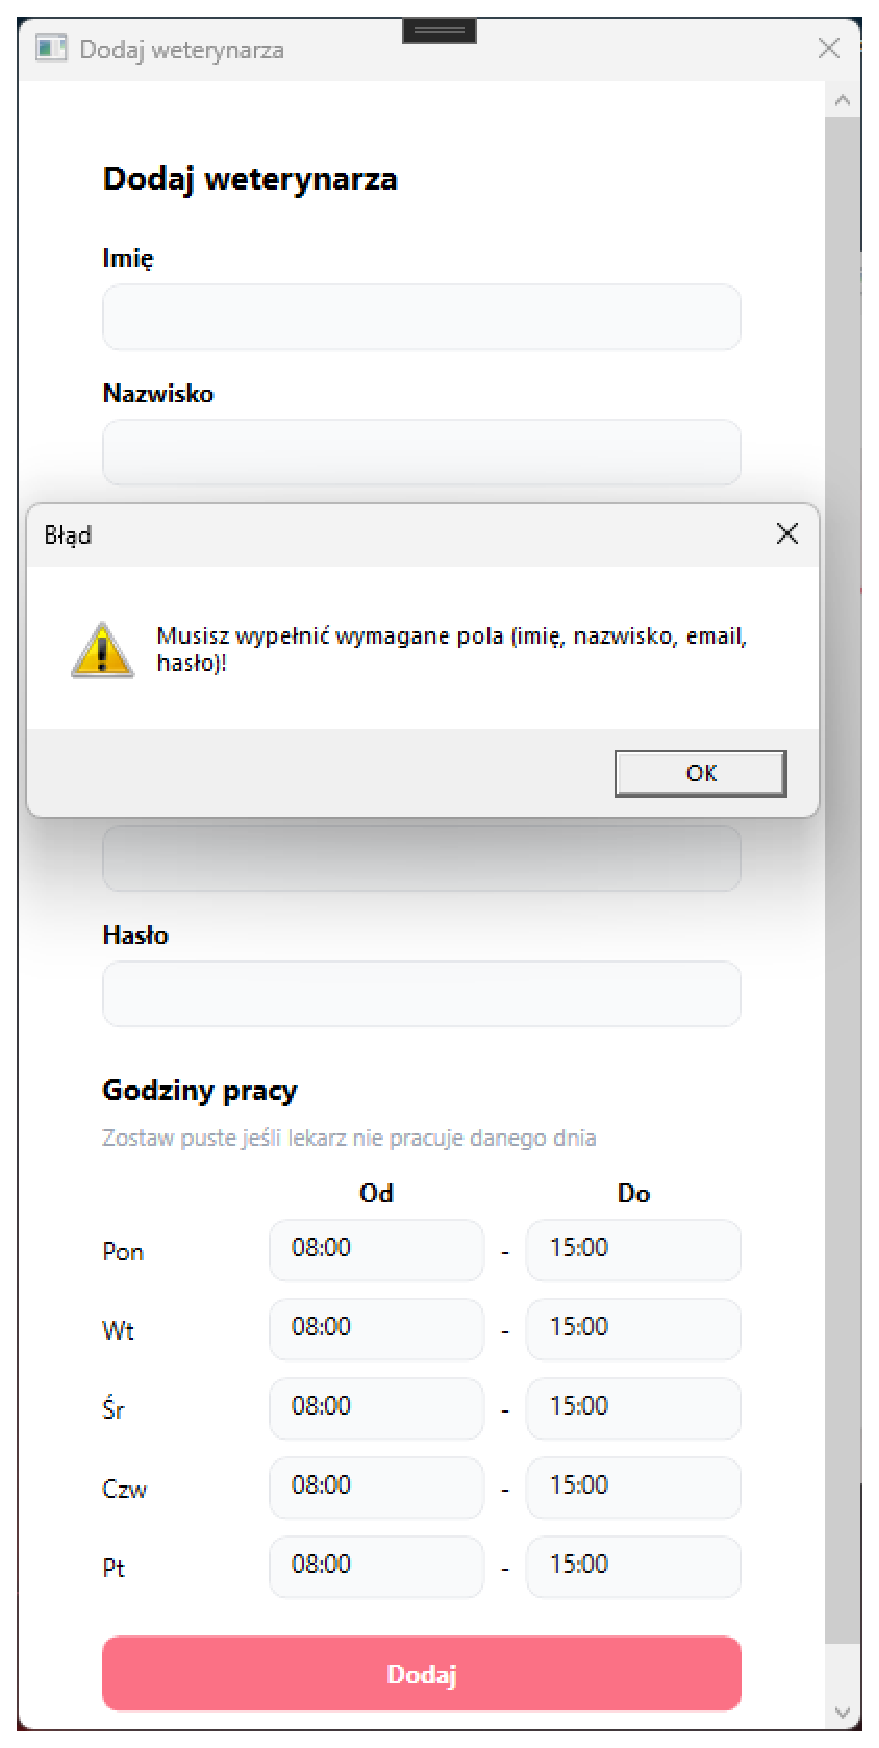
\includegraphics[width=0.6\linewidth]{figures/Admin/fig_042.eps}
\caption{Komunikat błędu przy niewypełnionych wymaganych polach.\label{fig42}}
\end{figure}

Po kliknięciu przycisku + przy wybranym weterynarzu otwierane jest okno zarządzania zabiegami. 
Wyświetlana jest lista wszystkich dostępnych zabiegów z checkboxami, zaznaczone zabiegi oznaczają te, 
które dany weterynarz aktualnie wykonuje. Administrator może dowolnie zaznaczać i odznaczać zabiegi, a następnie zapisać zmiany przyciskiem Zapisz.

\begin{figure}[H]
\centering
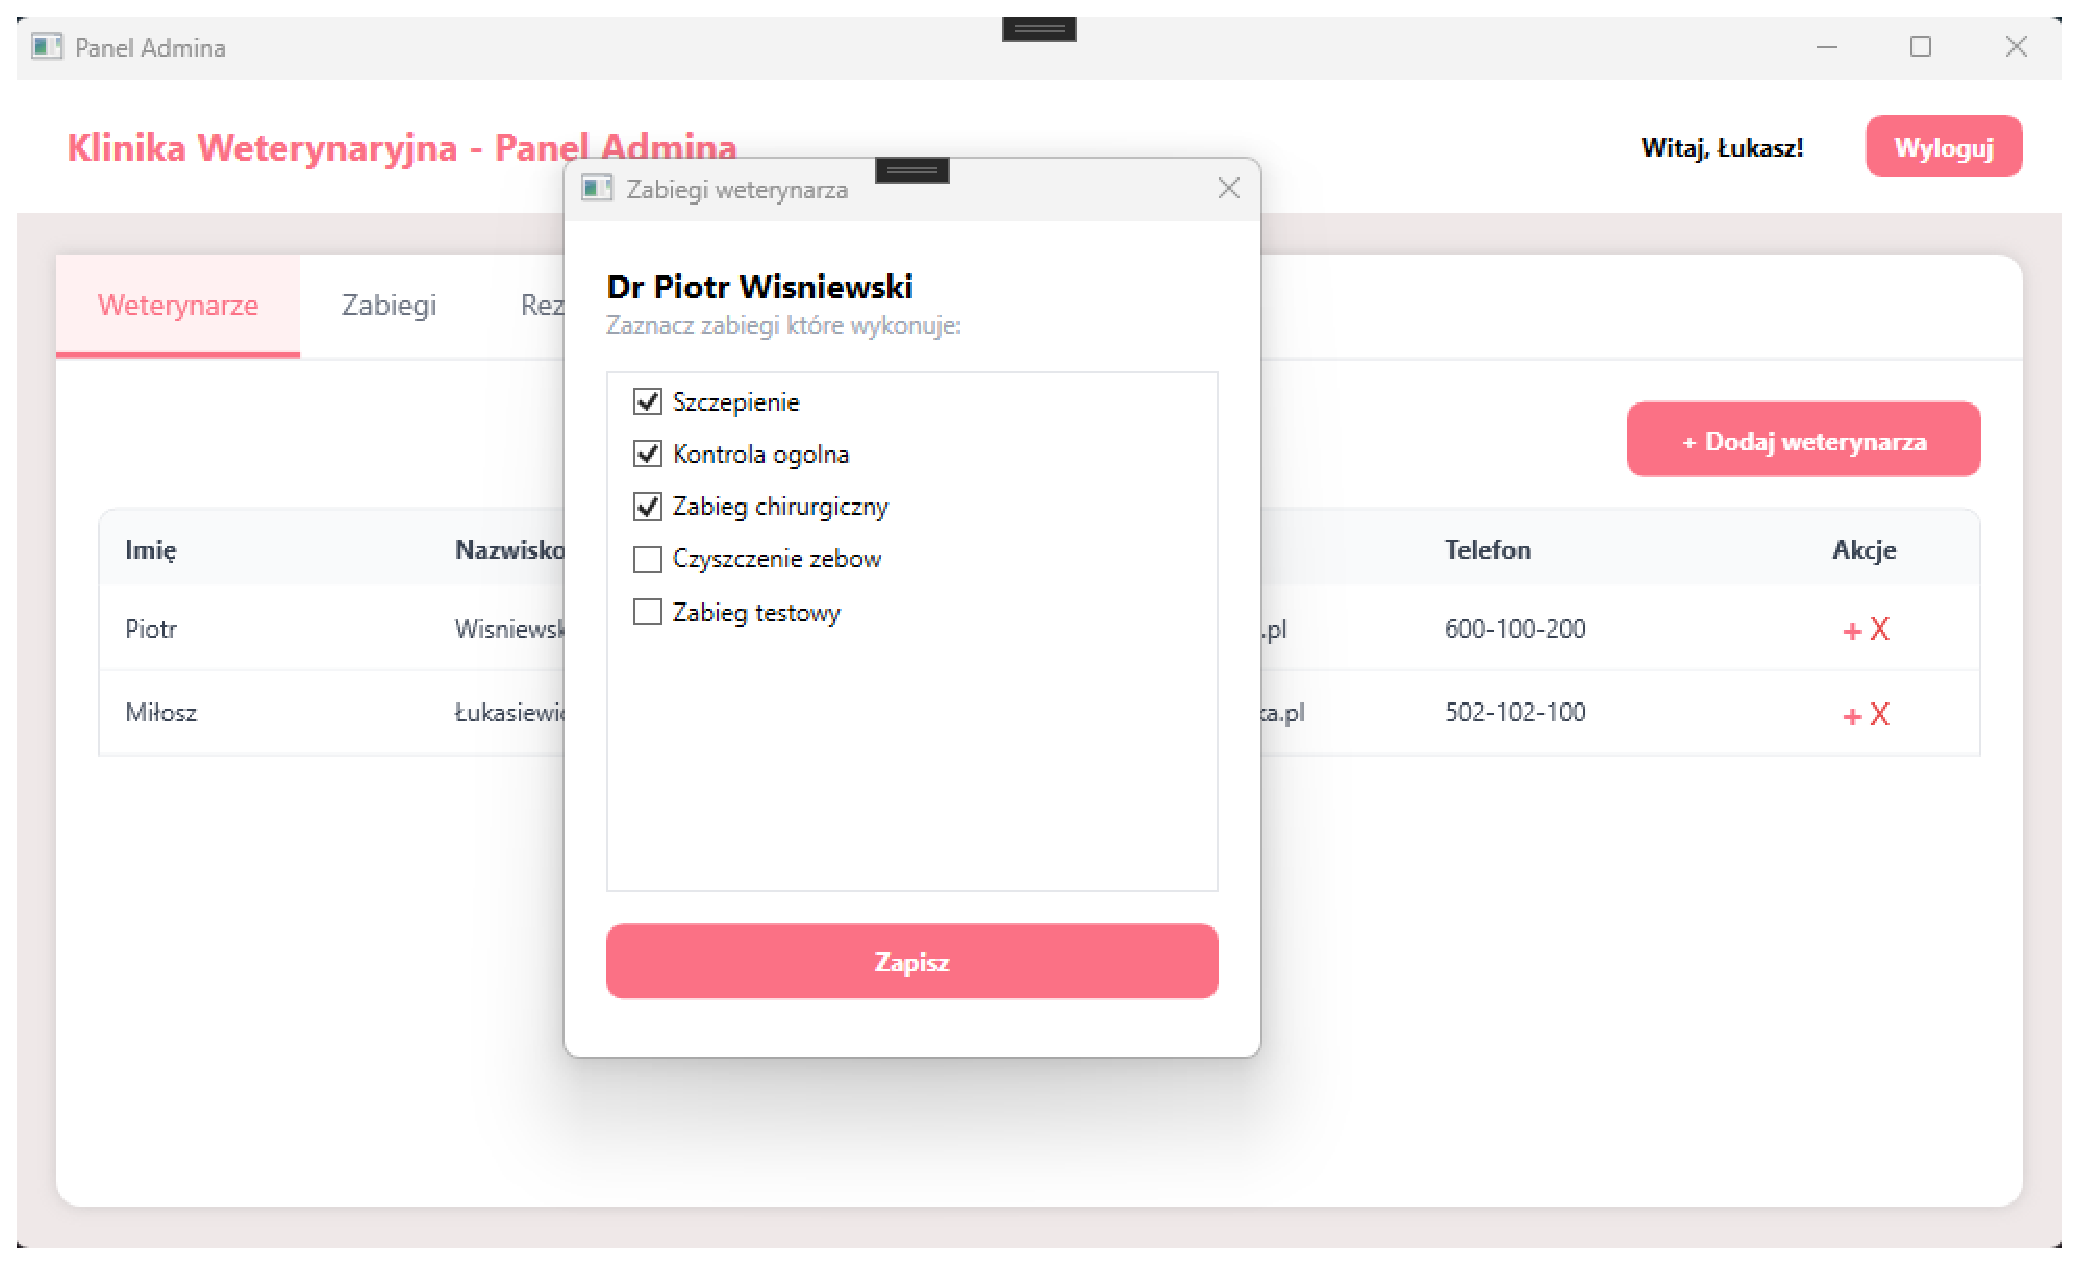
\includegraphics[width=0.9\linewidth]{figures/Admin/fig_043.eps}
\caption{Okno zarządzania zabiegami weterynarza.\label{fig43}}
\end{figure}

Po kliknięciu przycisku Zapisz aplikacja aktualizuje przypisanie zabiegów do weterynarza w bazie danych i 
wyświetla komunikat potwierdzający pomyślne wykonanie operacji.

\begin{figure}[H]
\centering
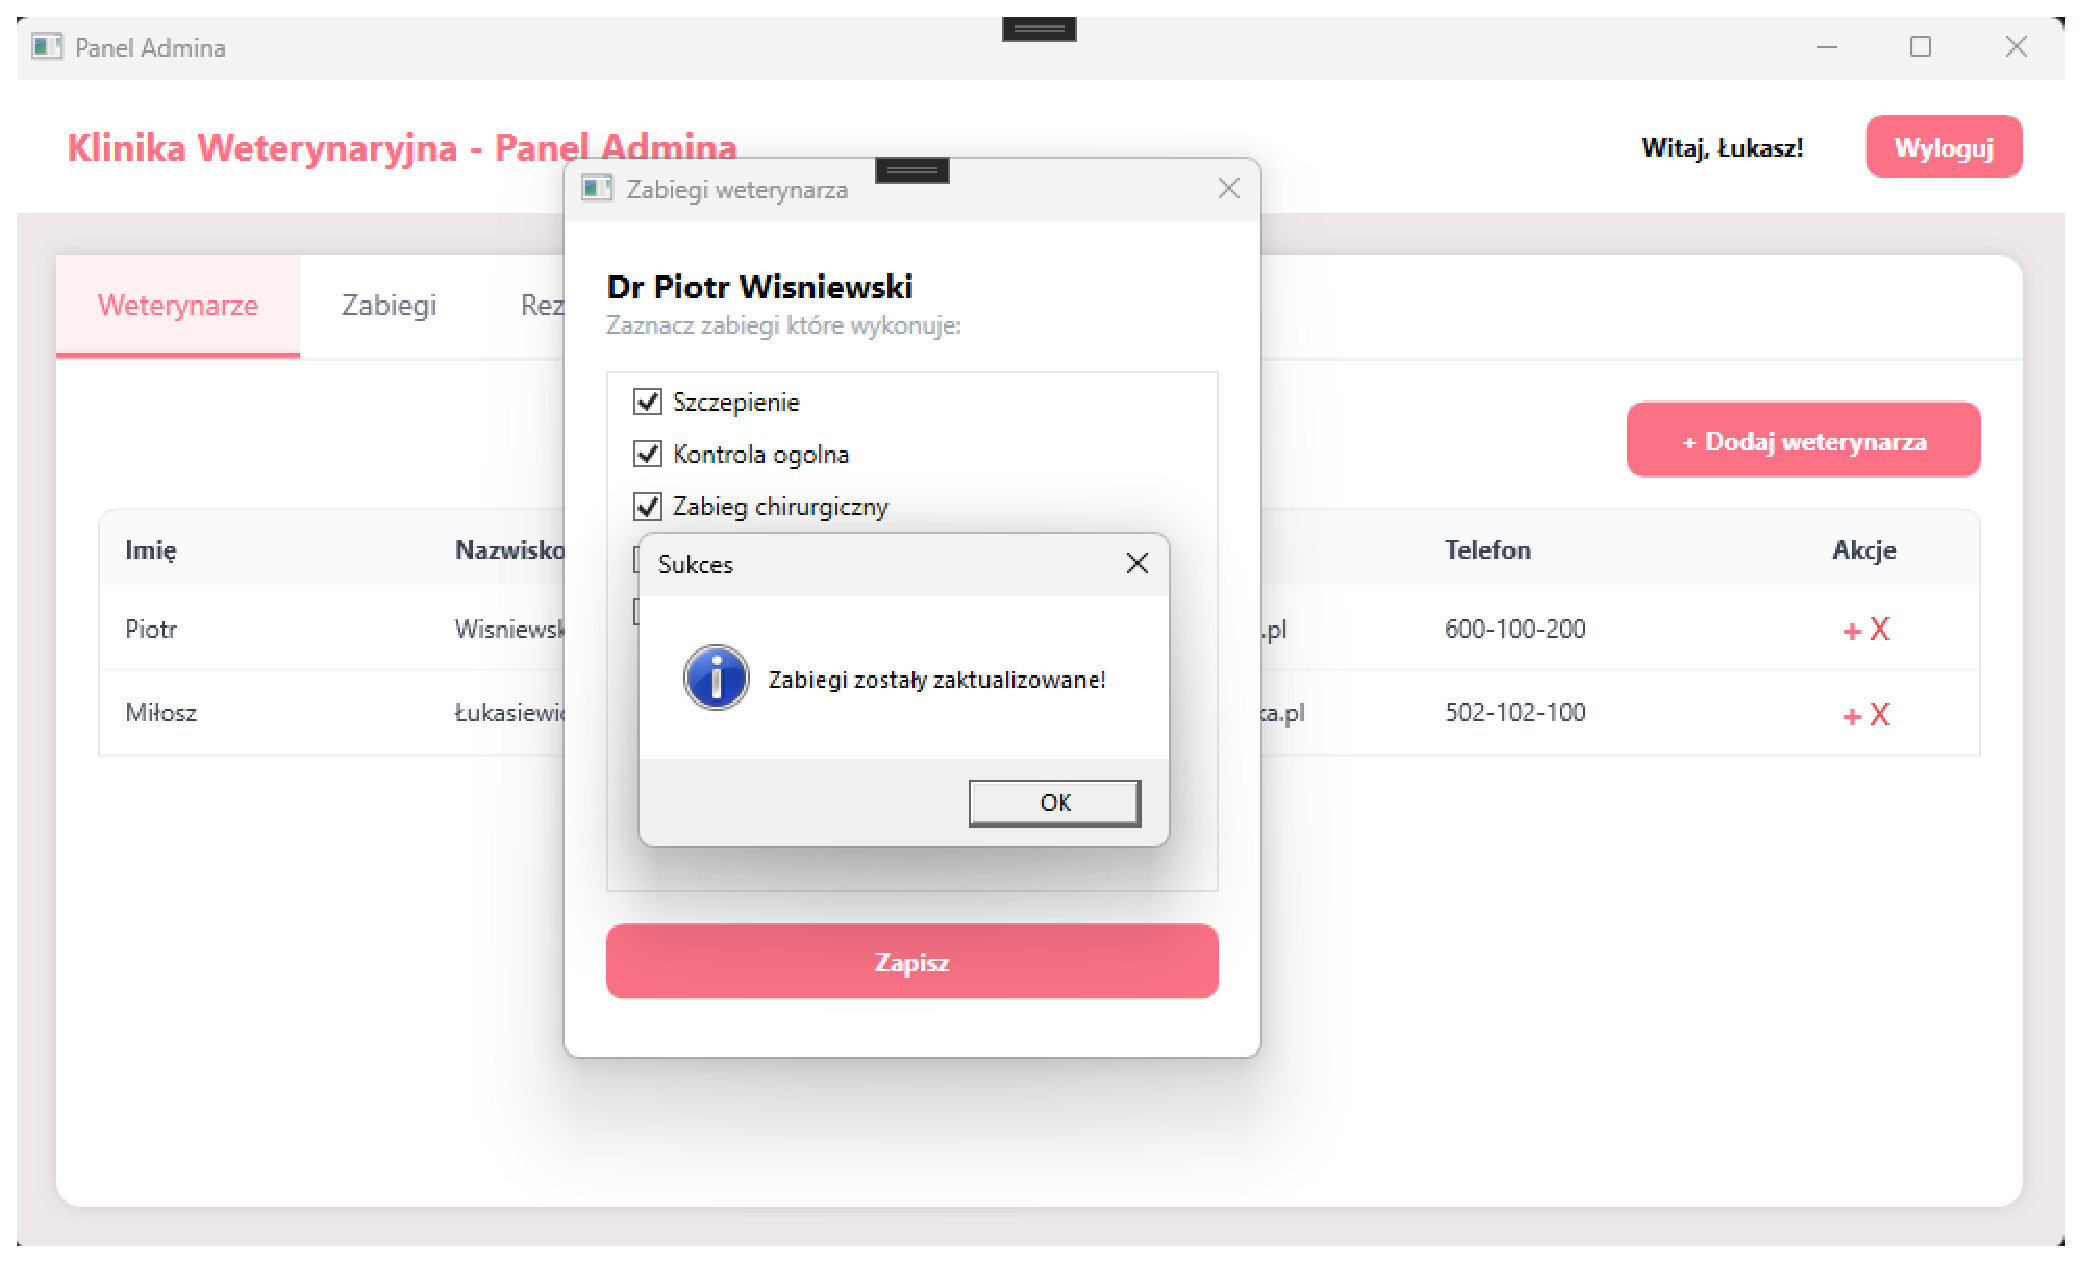
\includegraphics[width=0.9\linewidth]{figures/Admin/fig_044.eps}
\caption{Komunikat potwierdzający aktualizację zabiegów weterynarza.\label{fig44}}
\end{figure}

Po kliknięciu przycisku X przy wybranym weterynarzu aplikacja wyświetla okno dialogowe z prośbą o potwierdzenie operacji, 
informując że usunięcie weterynarza spowoduje również usunięcie jego dostępności i rezerwacji. 
Po potwierdzeniu weterynarz zostaje trwale usunięty z systemu.

\begin{figure}[H]
\centering
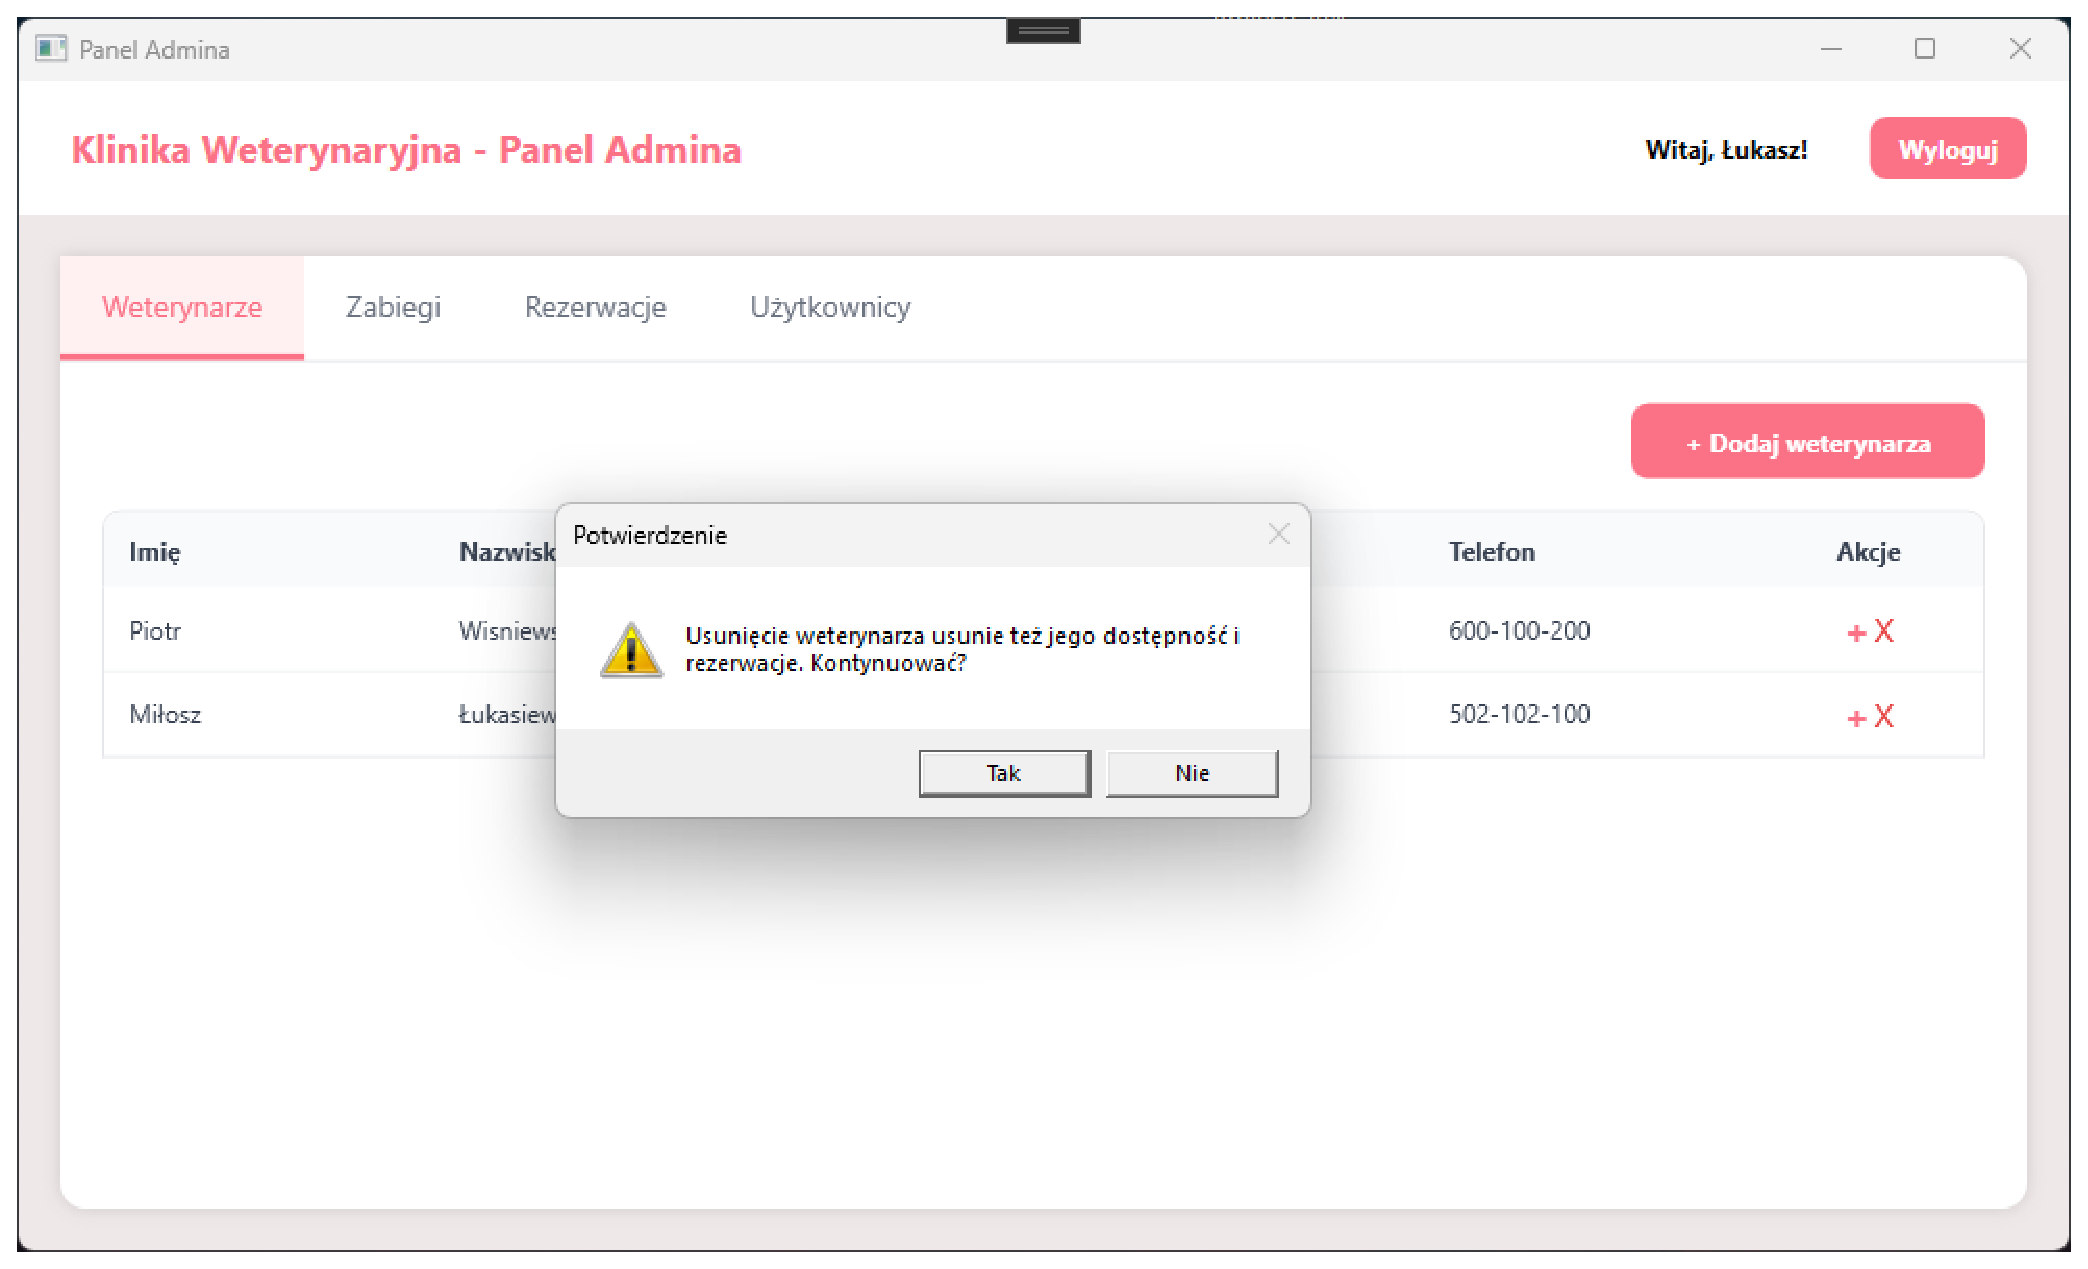
\includegraphics[width=0.9\linewidth]{figures/Admin/fig_045.eps}
\caption{Okno potwierdzenia usunięcia weterynarza.\label{fig45}}
\end{figure}

\textbf{Zakładka "Zabiegi"}

Zakładka "Zabiegi" wyświetla listę wszystkich zabiegów dostępnych w klinice. Dla każdego zabiegu prezentowane są 
informacje takie jak nazwa, czas trwania w minutach oraz cena. Przy każdym zabiegu dostępny jest przycisk X umożliwiający 
usunięcie zabiegu z systemu. W prawym górnym rogu zakładki znajduje się przycisk (+ Dodaj zabieg).

\begin{figure}[H]
\centering
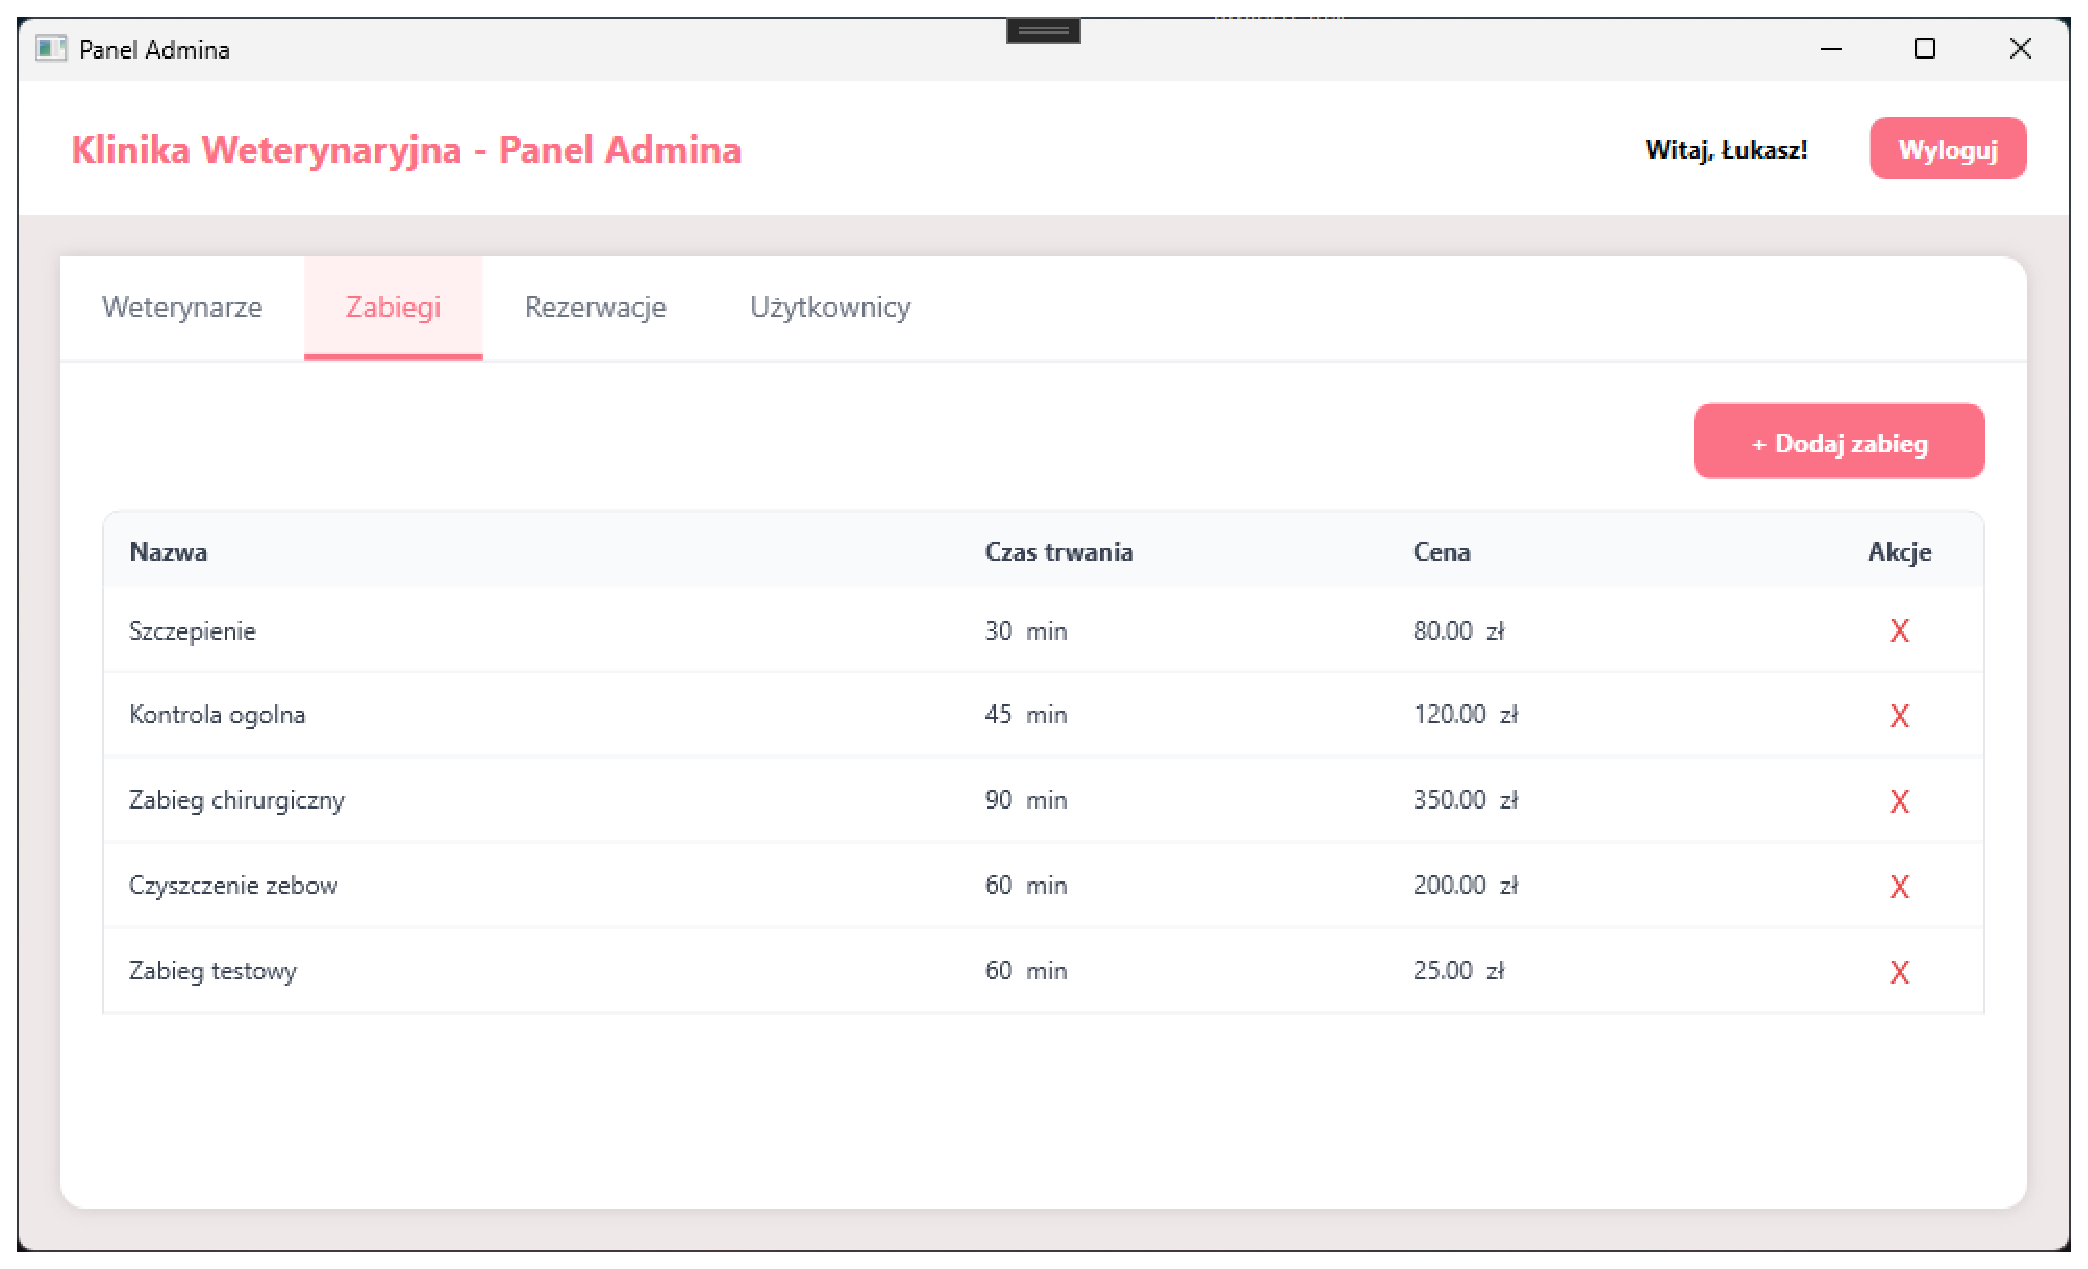
\includegraphics[width=0.9\linewidth]{figures/Admin/fig_046.eps}
\caption{Widok zakładki Zabiegi w panelu administratora.\label{fig46}}
\end{figure}

Po kliknięciu przycisku (+ Dodaj zabieg) otwierane jest okno formularza zawierające 
trzy pola: nazwa zabiegu, czas trwania w minutach oraz cena w złotych.

\begin{figure}[H]
\centering
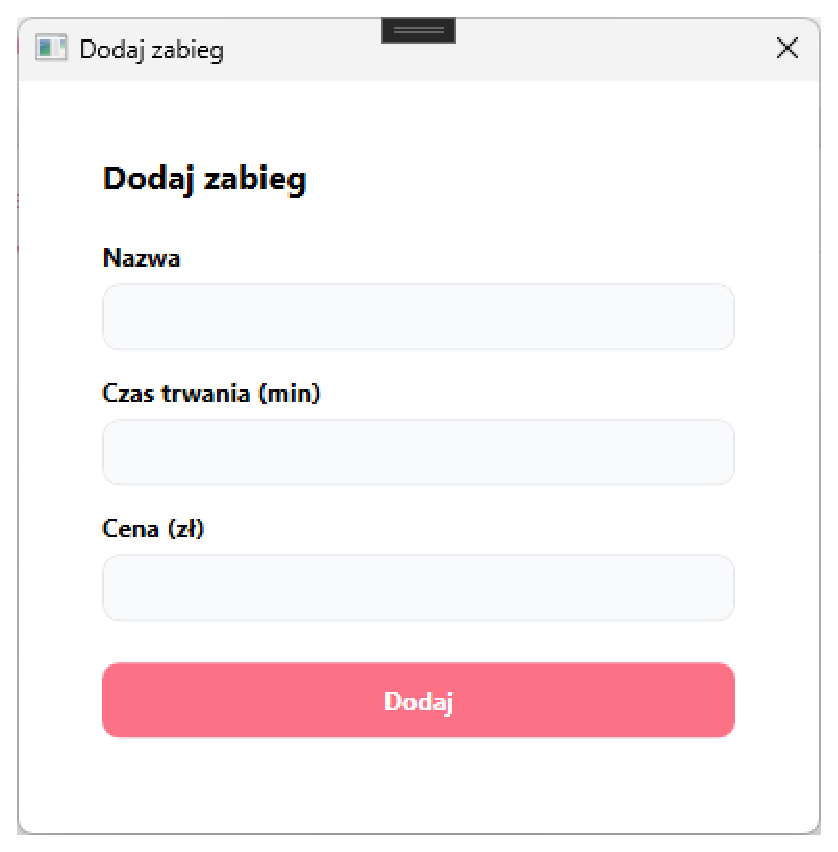
\includegraphics[width=0.55\linewidth]{figures/Admin/fig_047.eps}
\caption{Okno formularza dodawania zabiegu.\label{fig47}}
\end{figure}

W przypadku gdy administrator nie wypełni wszystkich pól formularza, aplikacja wyświetla komunikat błędu.

\begin{figure}[H]
\centering
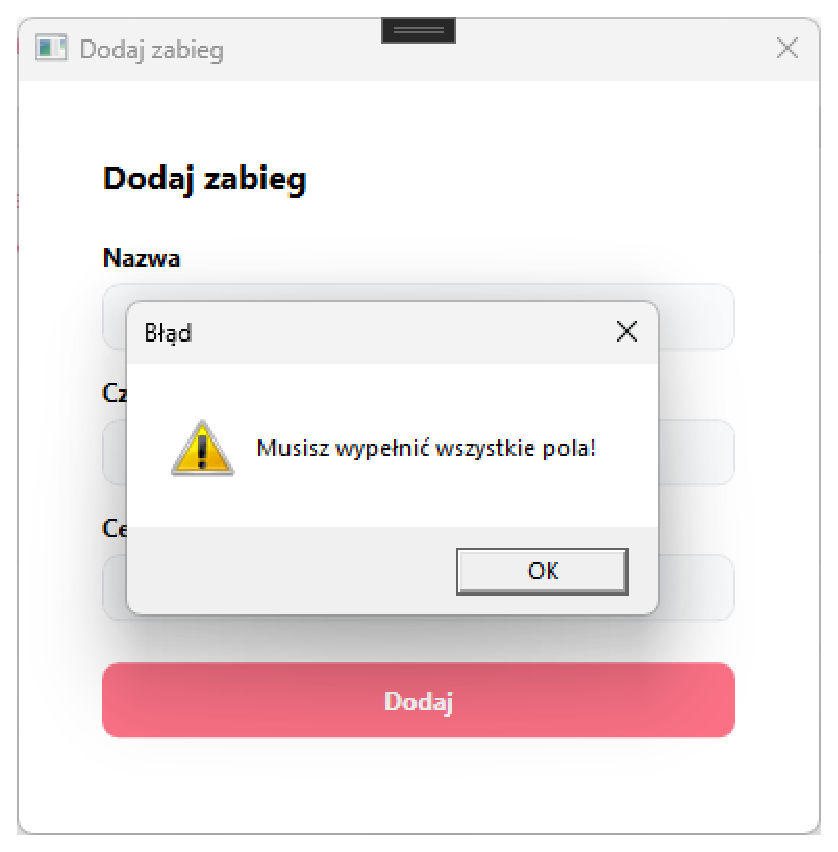
\includegraphics[width=0.55\linewidth]{figures/Admin/fig_048.eps}
\caption{Komunikat błędu przy niewypełnionych polach formularza.\label{fig48}}
\end{figure}

Aplikacja waliduje również poprawność podanego czasu trwania tzn. musi być dodatnią liczbą całkowitą. 
W przypadku podania nieprawidłowej wartości wyświetlany jest komunikat błędu.

\begin{figure}[H]
\centering
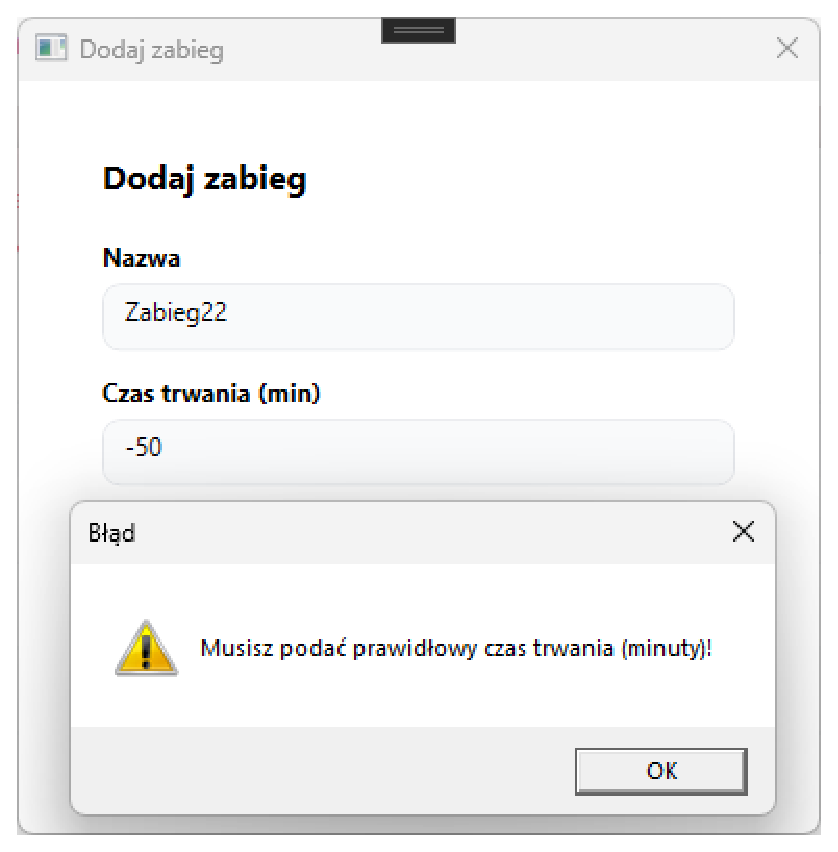
\includegraphics[width=0.55\linewidth]{figures/Admin/fig_049.eps}
\caption{Komunikat błędu przy nieprawidłowym czasie trwania zabiegu.\label{fig49}}
\end{figure}

Analogicznie walidowana jest cena zabiegu tzn. nie może być ona liczbą ujemną. W przypadku podania nieprawidłowej 
wartości wyświetlany jest odpowiedni komunikat błędu.

\begin{figure}[H]
\centering
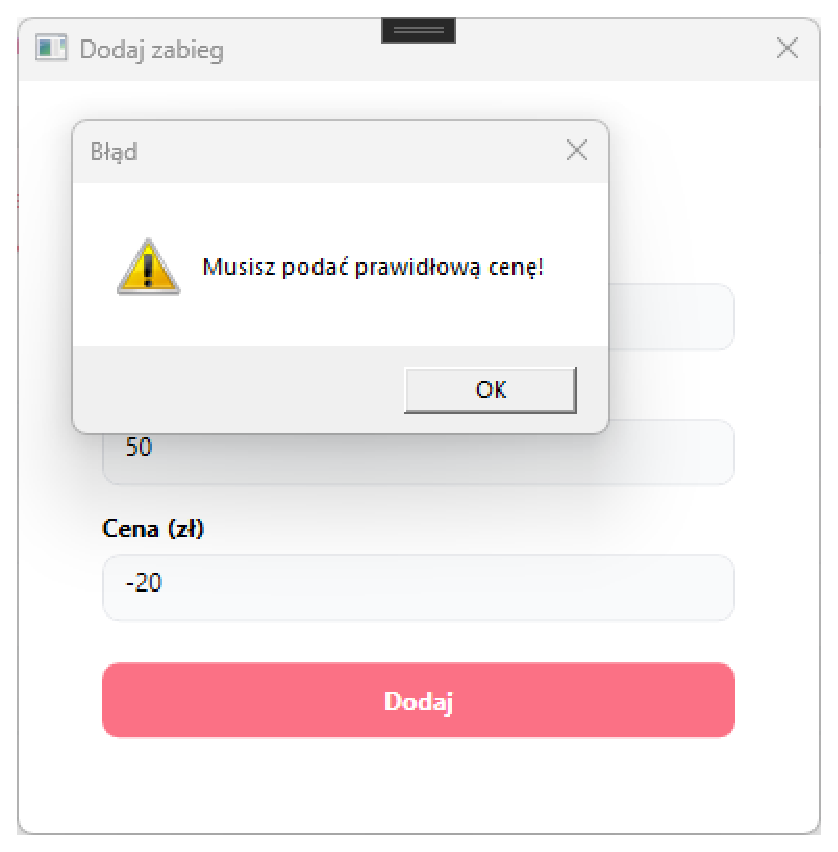
\includegraphics[width=0.55\linewidth]{figures/Admin/fig_050.eps}
\caption{Komunikat błędu przy nieprawidłowej cenie zabiegu.\label{fig50}}
\end{figure}

Po poprawnym wypełnieniu wszystkich pól i kliknięciu przycisku Dodaj nowy zabieg zostaje zapisany w bazie danych, a aplikacja 
wyświetla komunikat potwierdzający pomyślne dodanie zabiegu.

\begin{figure}[H]
\centering
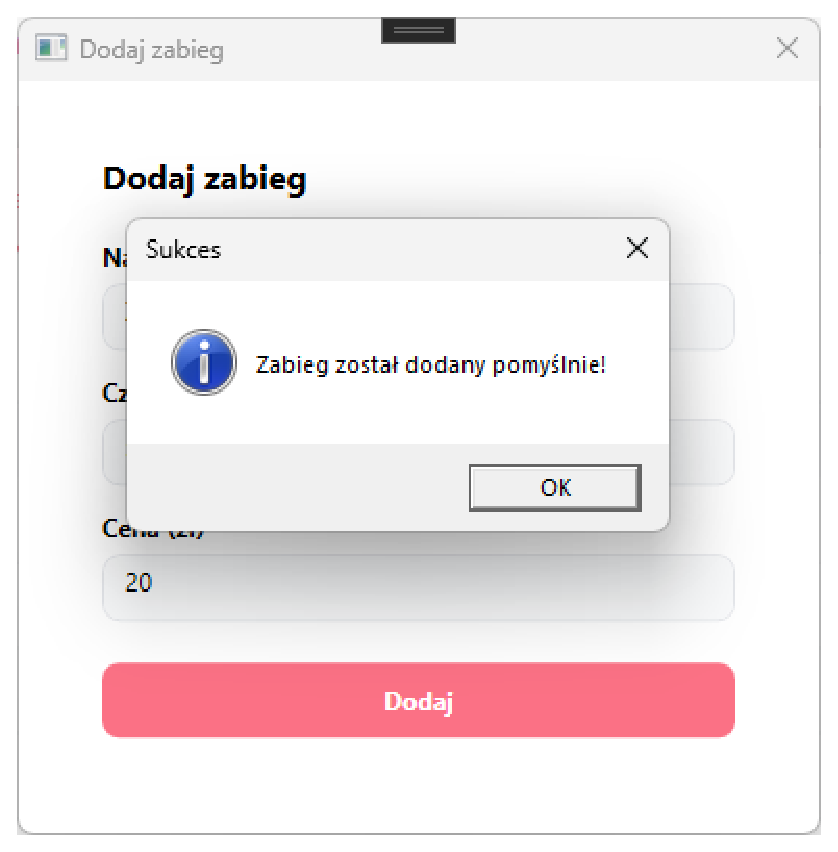
\includegraphics[width=0.55\linewidth]{figures/Admin/fig_051.eps}
\caption{Komunikat potwierdzający pomyślne dodanie zabiegu.\label{fig51}}
\end{figure}

Po kliknięciu przycisku X przy wybranym zabiegu aplikacja wyświetla okno dialogowe z prośbą o potwierdzenie operacji, informując 
że usunięcie zabiegu spowoduje również usunięcie powiązanych rezerwacji. Po potwierdzeniu zabieg zostaje trwale usunięty z systemu.

\begin{figure}[H]
\centering
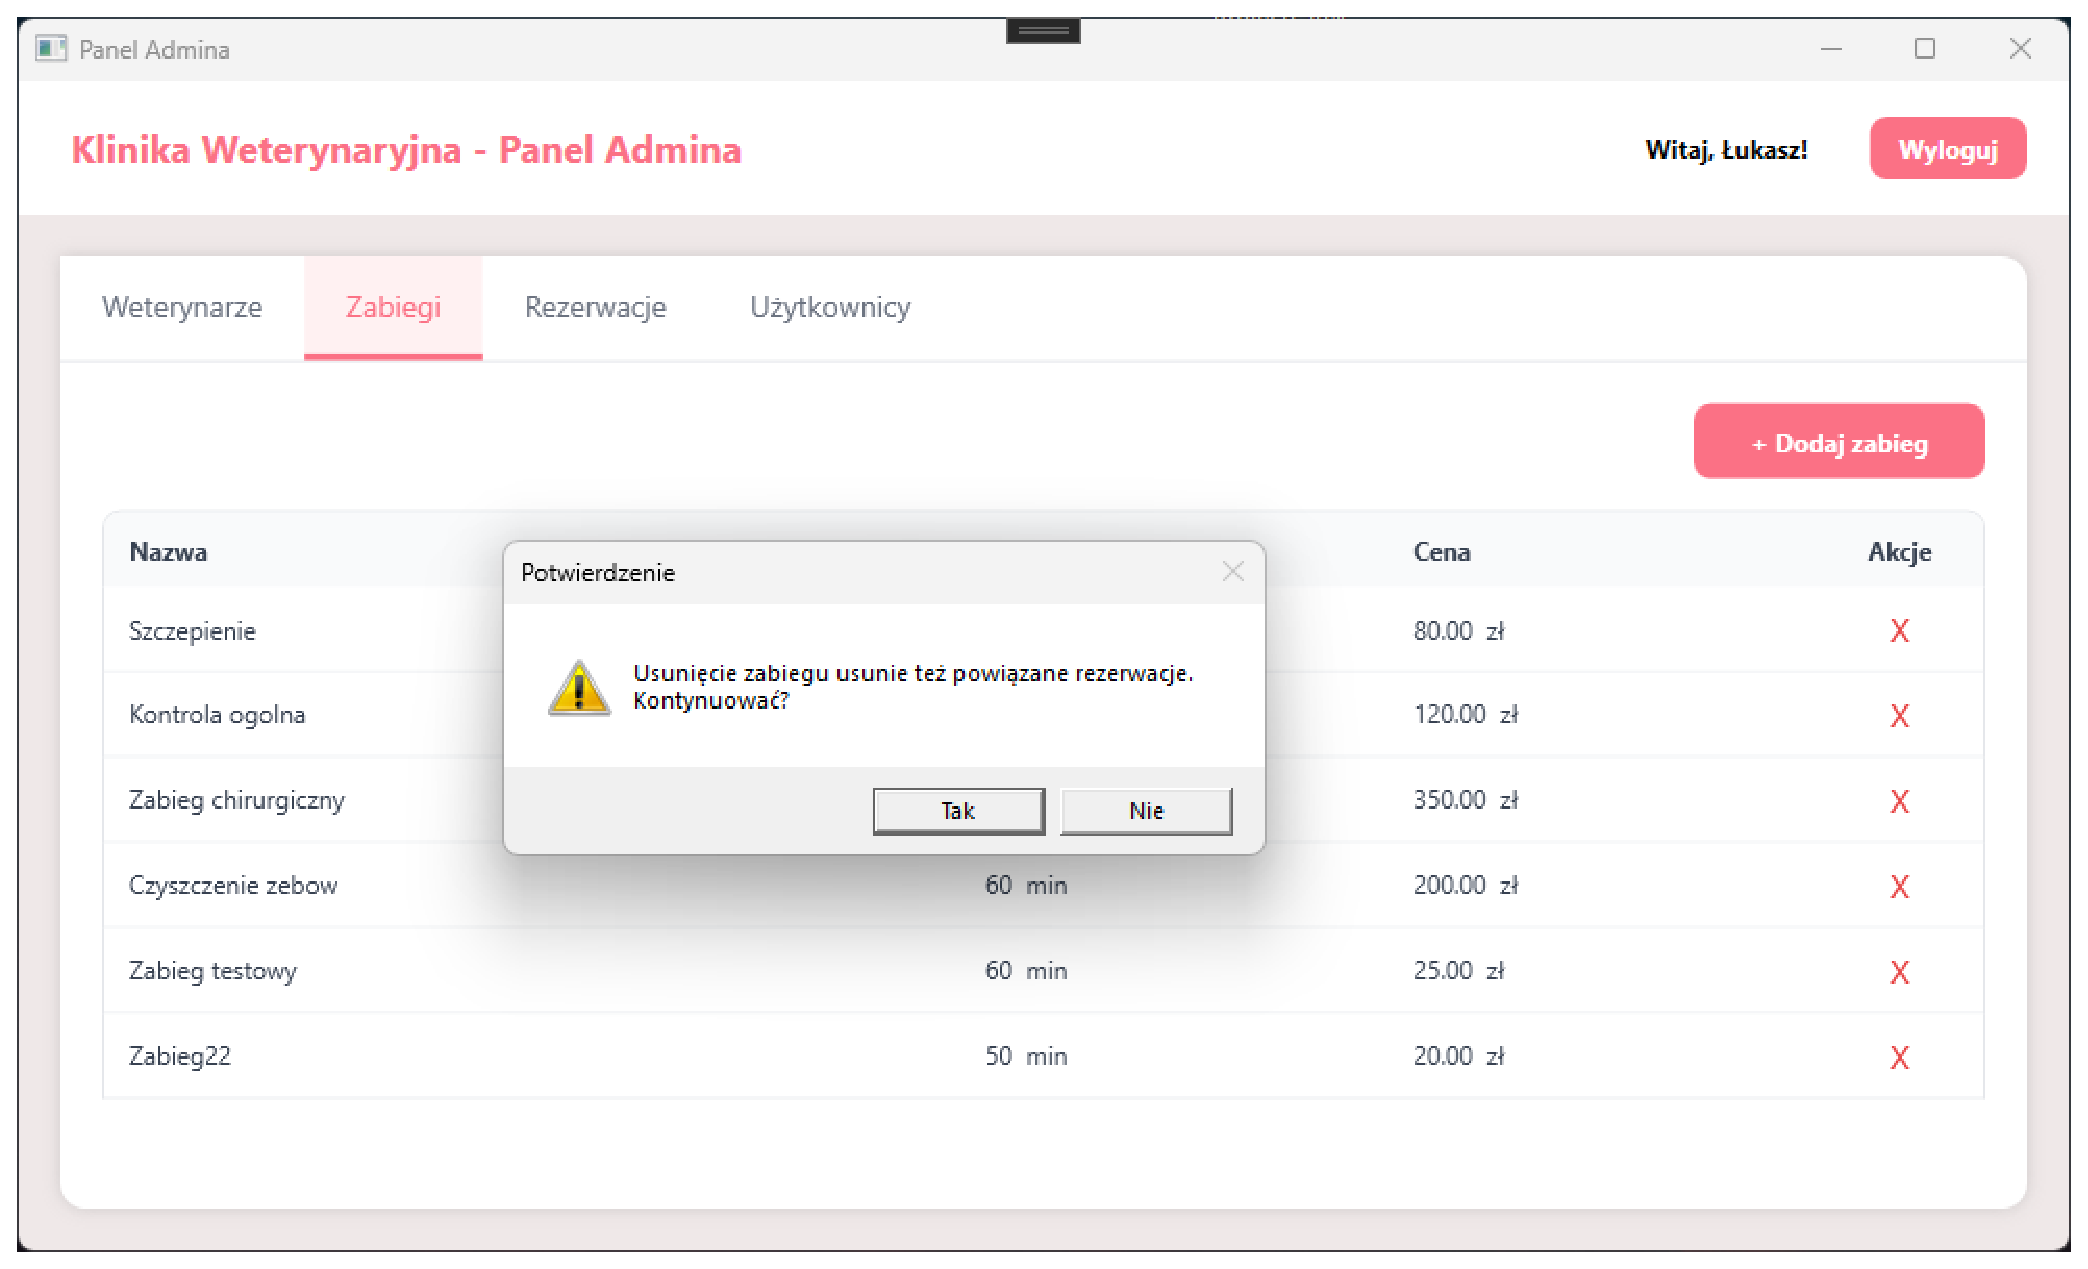
\includegraphics[width=0.9\linewidth]{figures/Admin/fig_052.eps}
\caption{Okno potwierdzenia usunięcia zabiegu.\label{fig52}}
\end{figure}

\textbf{Zakładka "Rezerwacje"}

Zakładka "Rezerwacje" wyświetla listę wszystkich rezerwacji wizyt w systemie. Dla każdej rezerwacji 
prezentowane są informacje takie jak data, godzina, imię i nazwisko weterynarza, imię pupila, nazwa zabiegu, imię i nazwisko 
właściciela oraz aktualny status wizyty. Administrator może zmieniać status każdej rezerwacji bezpośrednio z poziomu listy przy użyciu 
listy rozwijanej z trzema opcjami: Zarezerwowany, Zrealizowany oraz Anulowany. Nad listą dostępne są 
filtry: filtr daty, filtr weterynarza oraz filtr statusu, a także przycisk Wyczyść filtry resetujący wszystkie filtry do wartości domyślnych.

\begin{figure}[H]
\centering
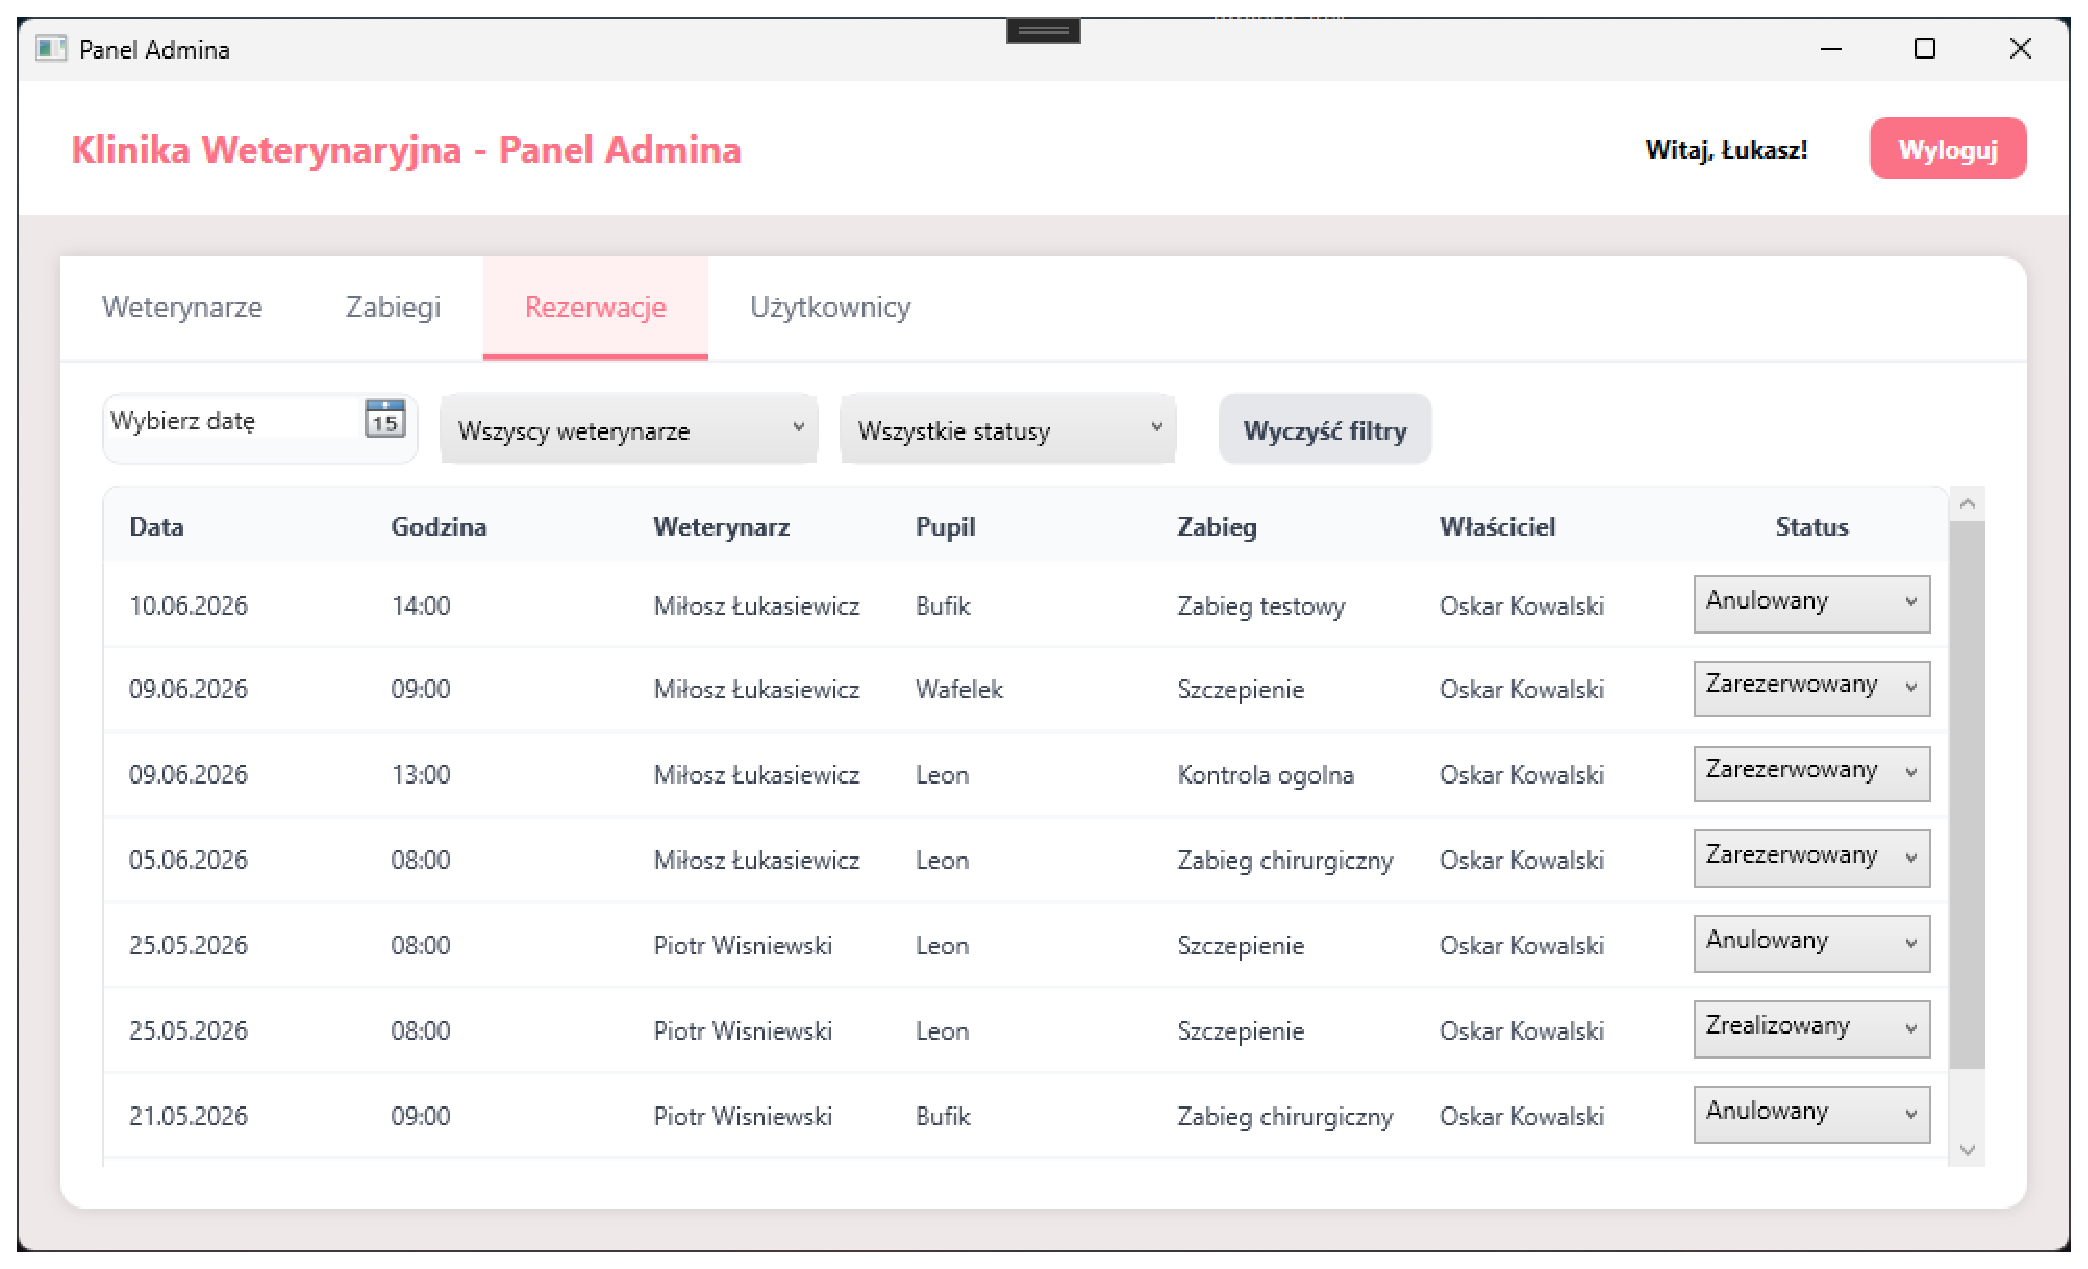
\includegraphics[width=0.9\linewidth]{figures/Admin/fig_053.eps}
\caption{Widok zakładki Rezerwacje w panelu administratora.\label{fig53}}
\end{figure}

Filtr daty umożliwia wyświetlenie wyłącznie rezerwacji z wybranego dnia. Poniżej przedstawiono widok po zastosowaniu 
filtra daty na dzień 25.05.2026 czyli lista zawiera tylko rezerwacje z tego dnia.

\begin{figure}[H]
\centering
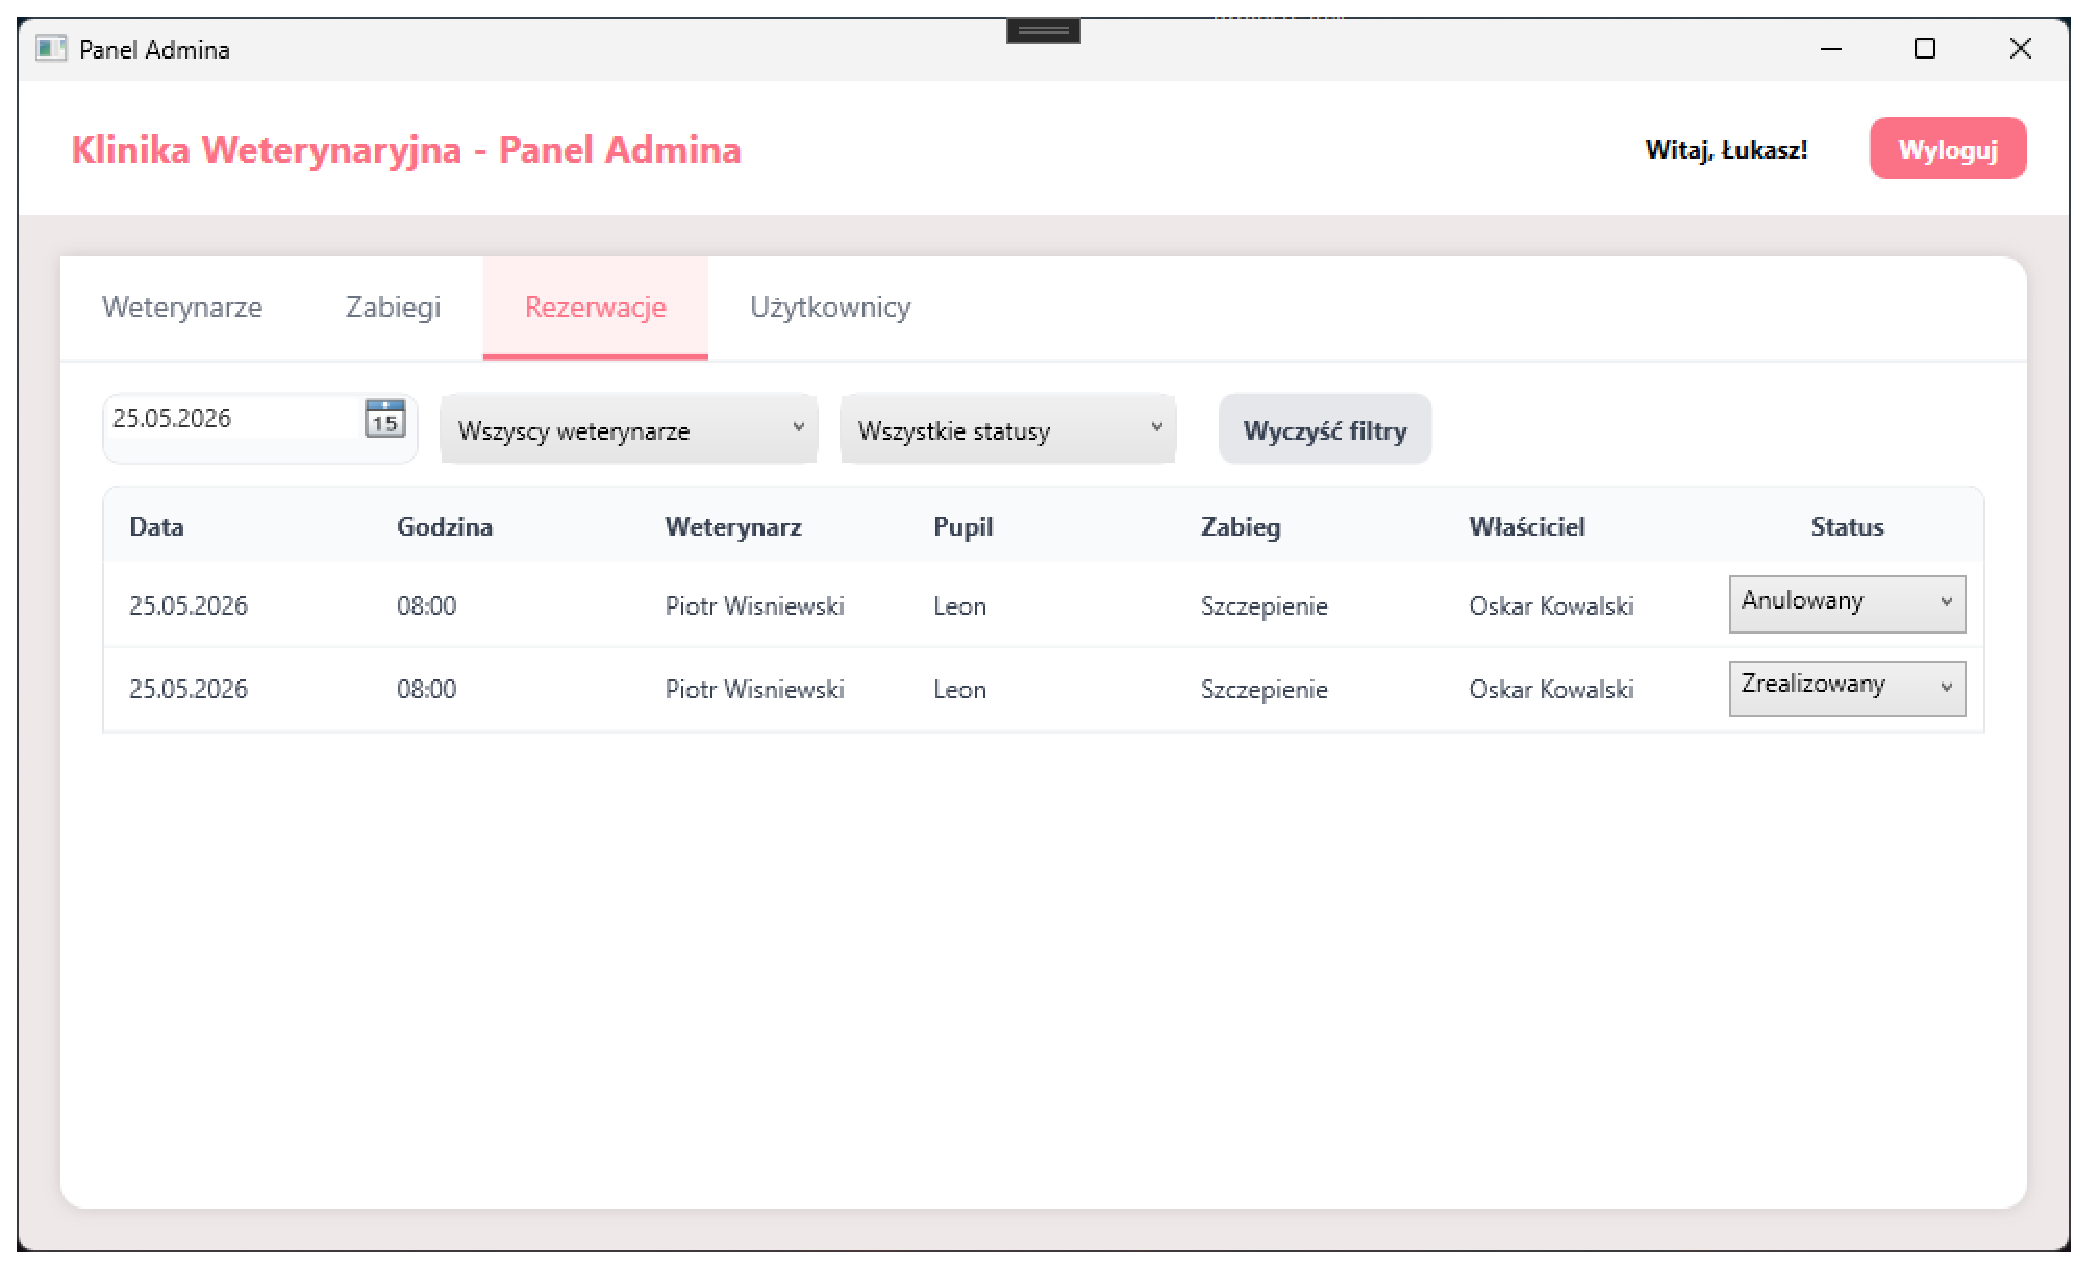
\includegraphics[width=0.9\linewidth]{figures/Admin/fig_054.eps}
\caption{Widok zakładki Rezerwacje po filtrowaniu po dacie.\label{fig54}}
\end{figure}

Filtr weterynarza umożliwia wyświetlenie wyłącznie rezerwacji przypisanych do wybranego weterynarza. 
Poniżej przedstawiono widok po wybraniu weterynarza Miłosz Łukasiewicz czyli lista zawiera tylko jego rezerwacje.

\begin{figure}[H]
\centering
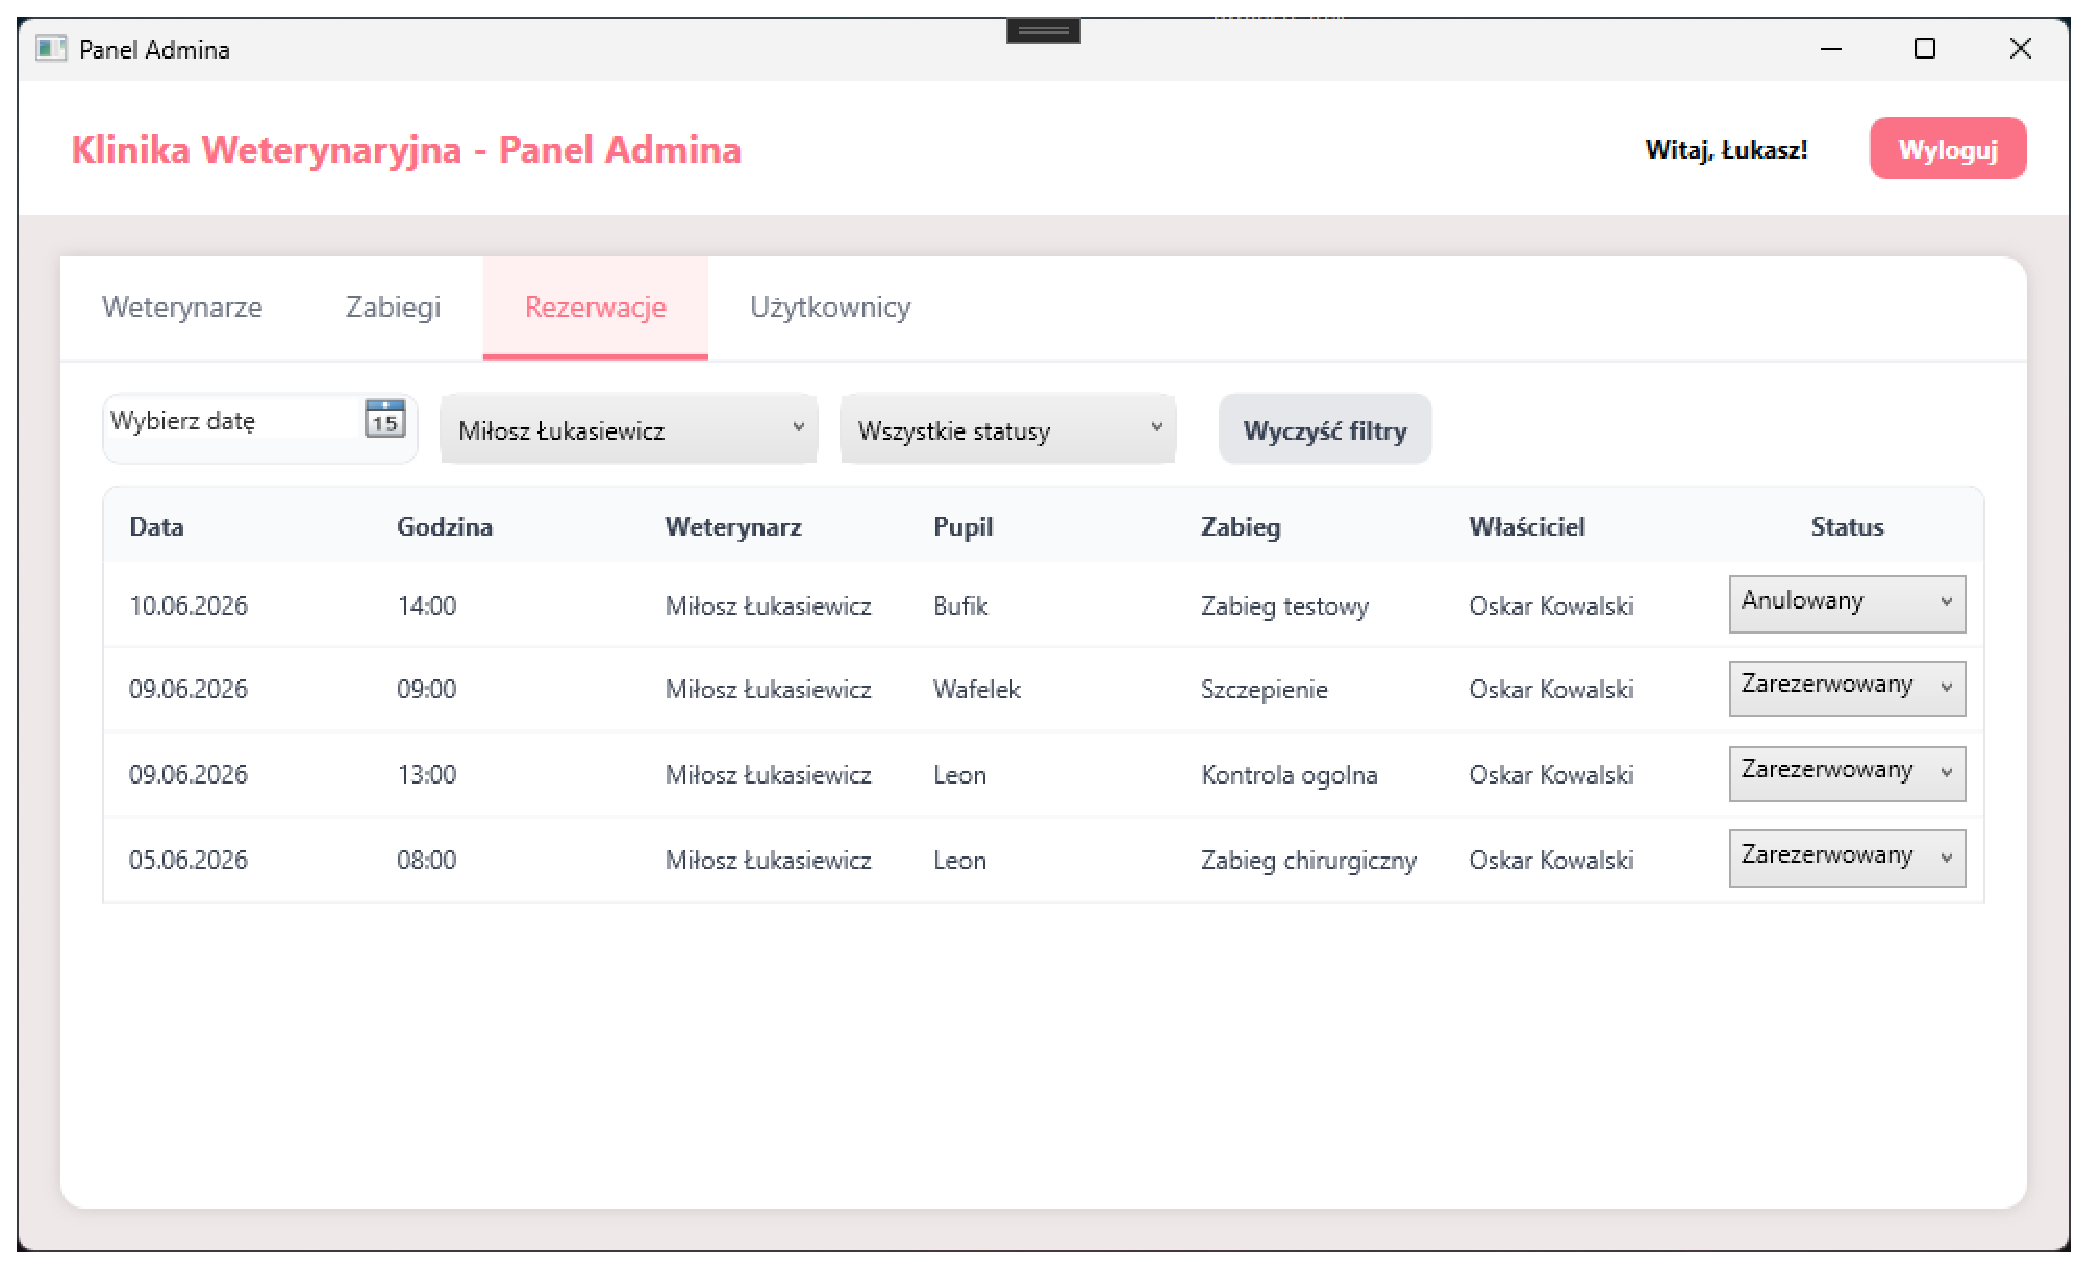
\includegraphics[width=0.9\linewidth]{figures/Admin/fig_055.eps}
\caption{Widok zakładki Rezerwacje po filtrowaniu po weterynarzu.\label{fig55}}
\end{figure}

Filtry można łączyć, poniżej przedstawiono widok po jednoczesnym zastosowaniu 
filtra weterynarza (Miłosz Łukasiewicz) oraz filtra statusu (Anulowany), co pozwala 
precyzyjnie odnaleźć konkretne rezerwacje spełniające oba kryteria.

\begin{figure}[H]
\centering
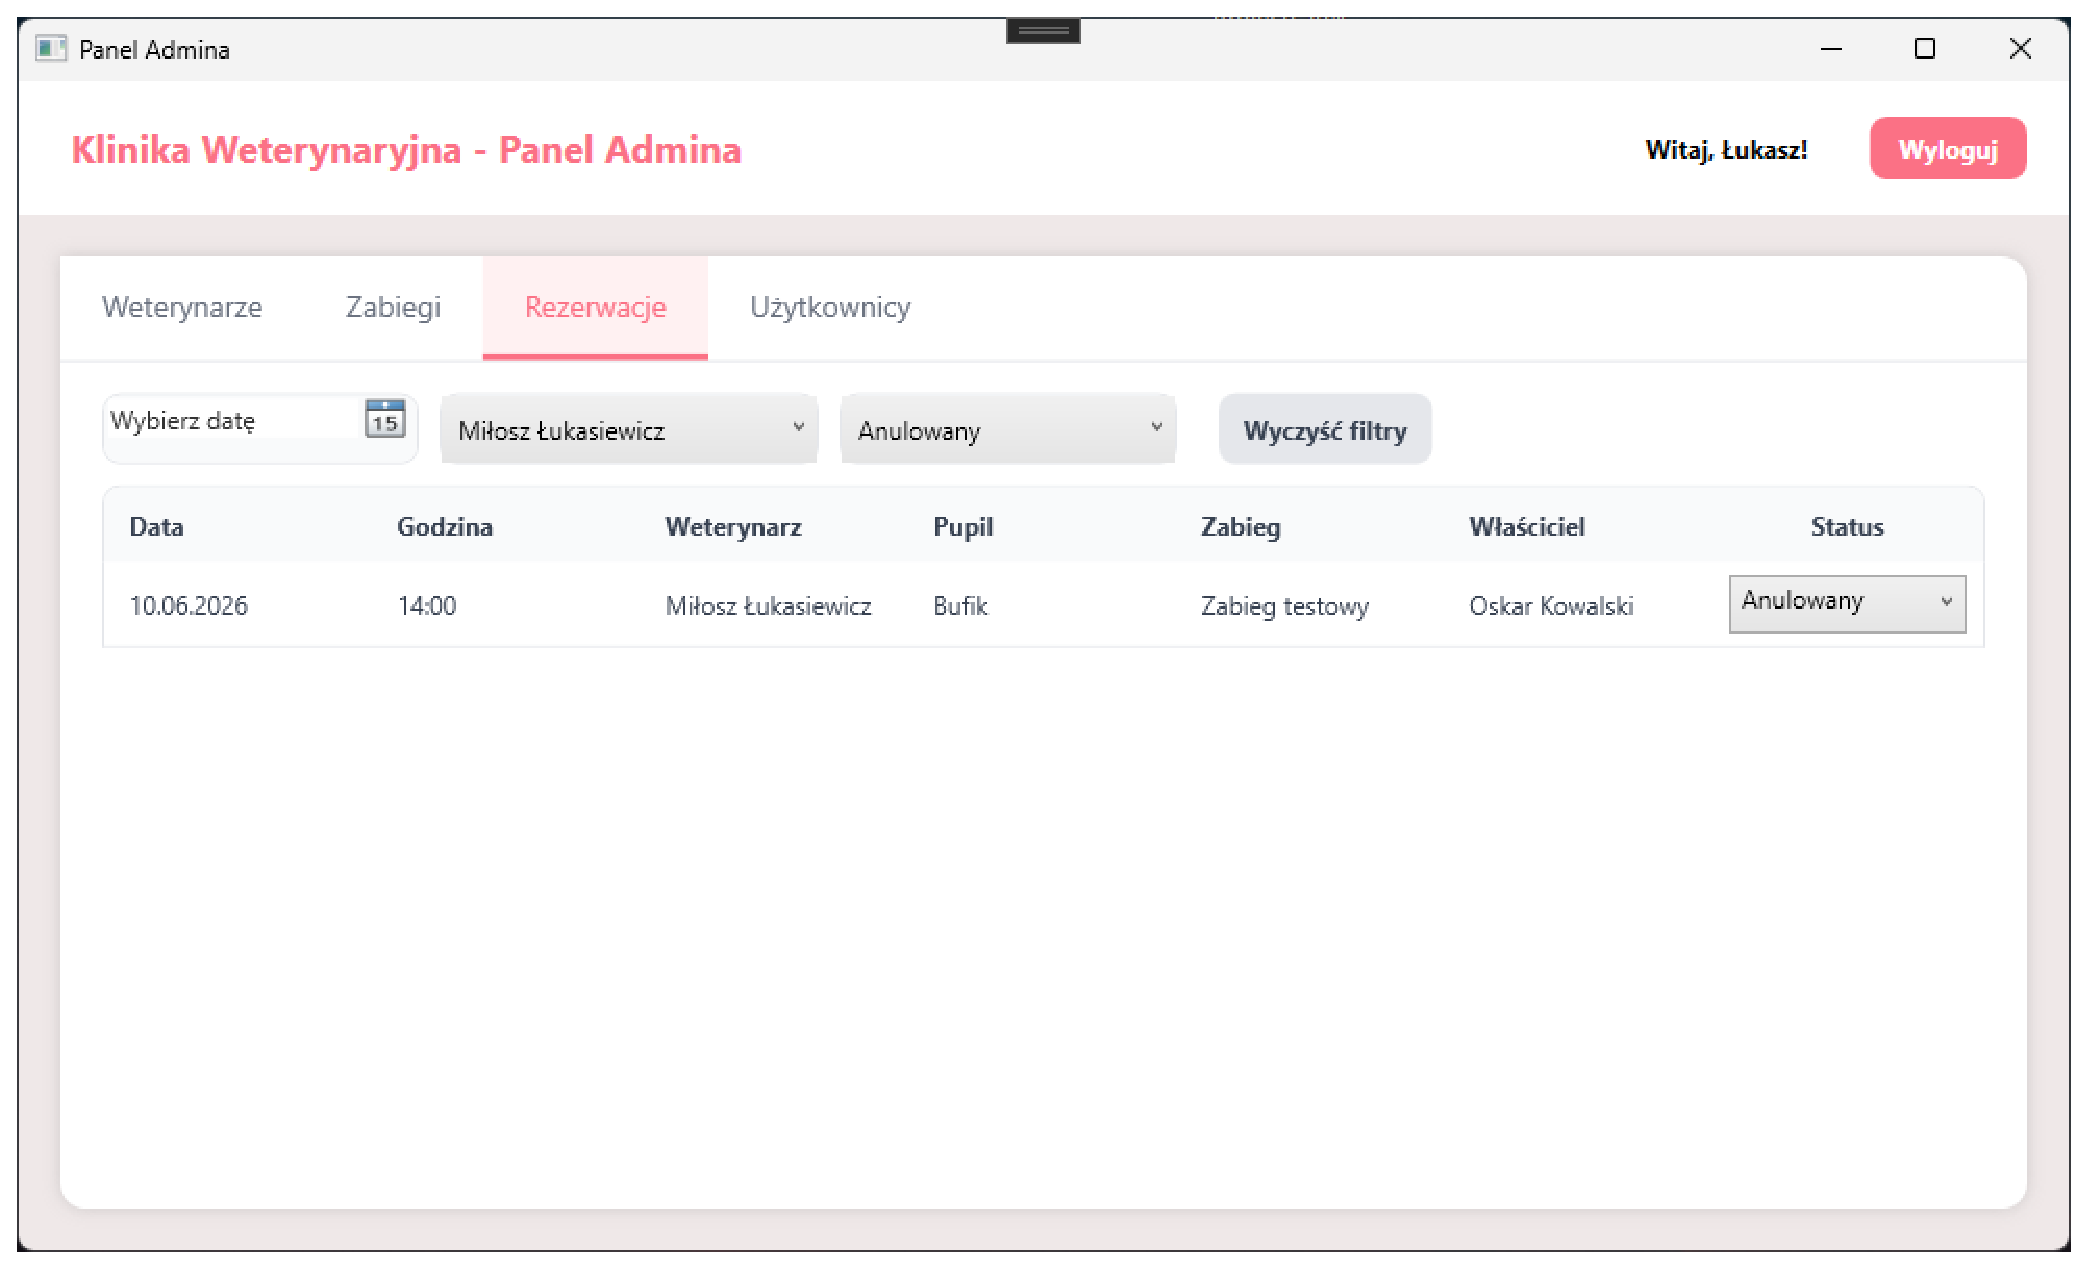
\includegraphics[width=0.9\linewidth]{figures/Admin/fig_056.eps}
\caption{Widok zakładki Rezerwacje po filtrowaniu po weterynarzu i statusie.\label{fig56}}
\end{figure}

\textbf{Zakładka "Użytkownicy"}

Zakładka "Użytkownicy" wyświetla listę wszystkich zarejestrowanych użytkowników systemu z rolą Uzytkownik. Dla każdego 
użytkownika prezentowane są informacje takie jak imię, nazwisko, adres e-mail, numer telefonu oraz aktualne saldo konta. 
Przy każdym użytkowniku dostępny jest przycisk X umożliwiający usunięcie użytkownika z systemu.

\begin{figure}[H]
\centering
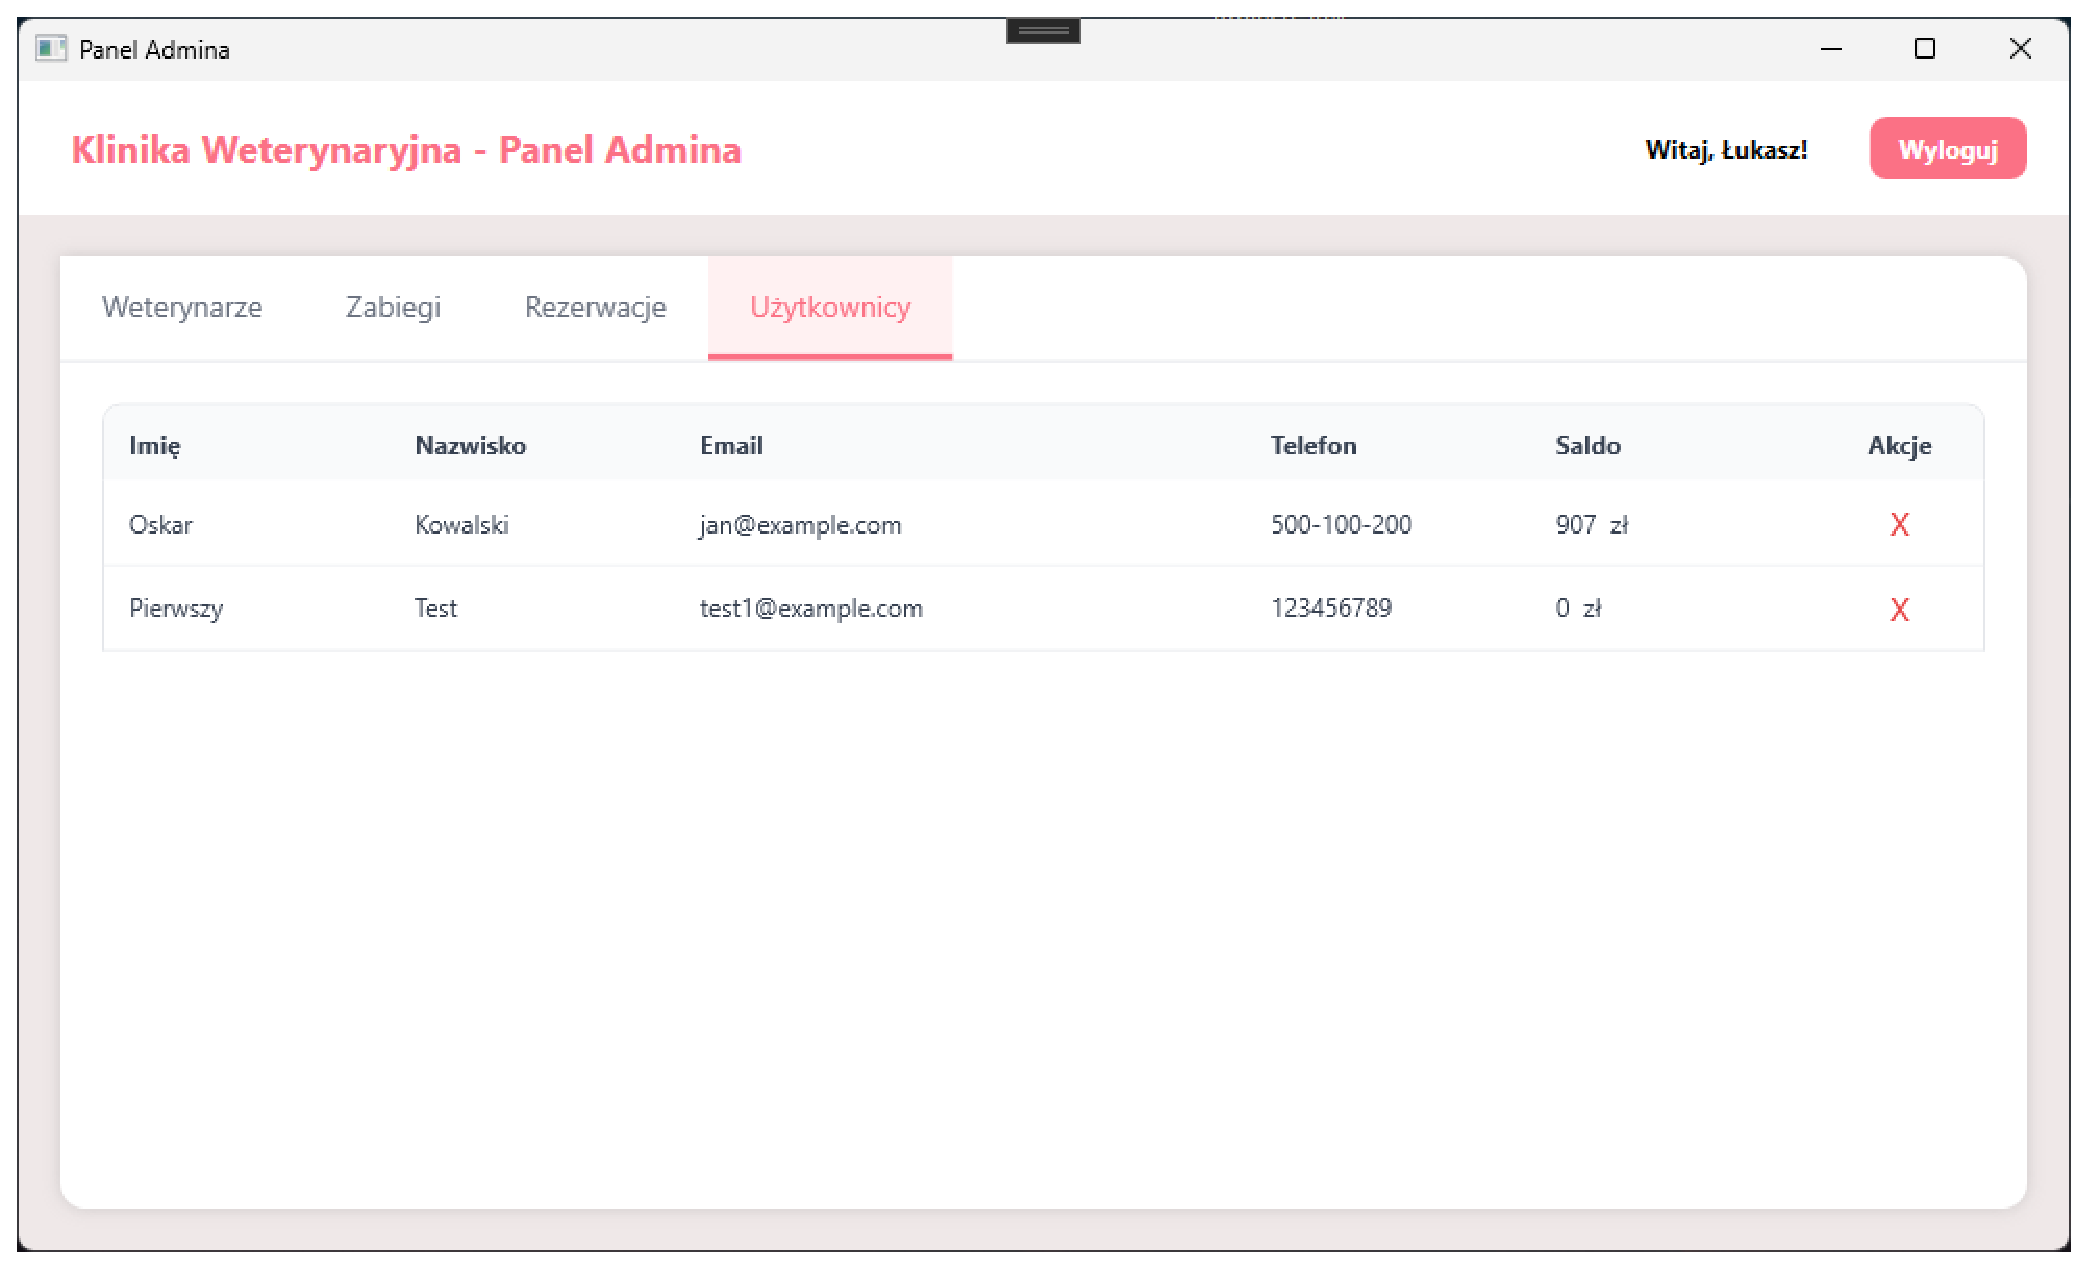
\includegraphics[width=0.9\linewidth]{figures/Admin/fig_057.eps}
\caption{Widok zakładki Użytkownicy w panelu administratora.\label{fig57}}
\end{figure}

Po kliknięciu przycisku X przy wybranym użytkowniku aplikacja wyświetla okno dialogowe z prośbą o 
potwierdzenie operacji, informując że usunięcie użytkownika spowoduje również usunięcie 
jego pupili i rezerwacji. Po potwierdzeniu użytkownik zostaje trwale usunięty z systemu 
wraz ze wszystkimi powiązanymi danymi, a lista użytkowników jest automatycznie odświeżana.

\begin{figure}[H]
\centering
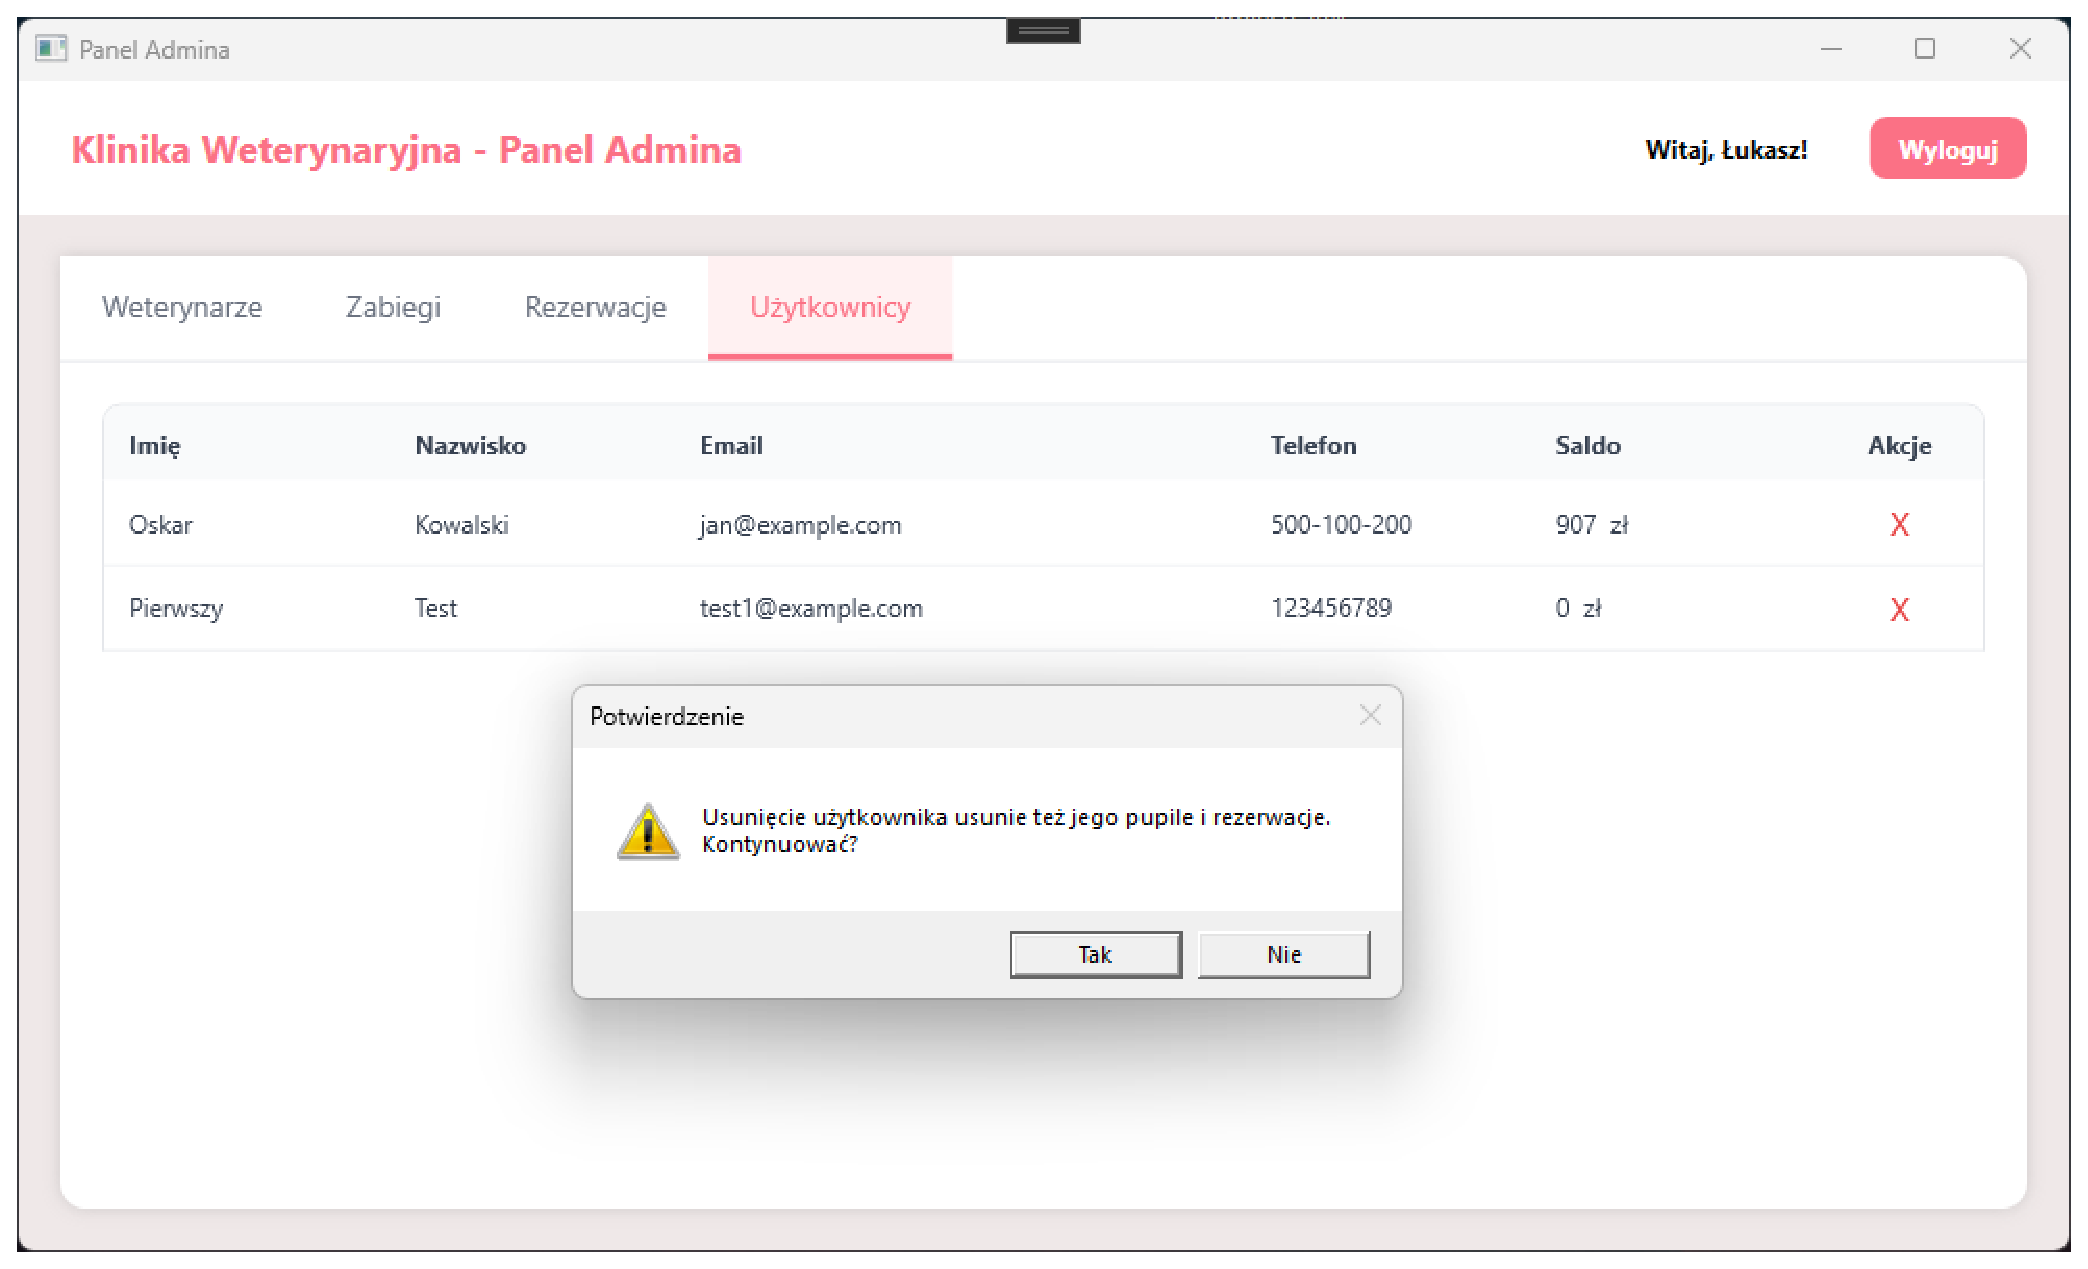
\includegraphics[width=0.9\linewidth]{figures/Admin/fig_058.eps}
\caption{Okno potwierdzenia usunięcia użytkownika.\label{fig58}}
\end{figure}

\section{Uruchomienie aplikacji}

\begin{enumerate}
\item Sklonować/Pobrać repozytorium projektu z GitHub: 
\url{https://github.com/lukaszwarzocha/Programowanie_Obiektowe2.git}
\item Otworzyć folder Projekt\_PO\_KW w Visual Studio Insiders.
\item Utworzyć bazę danych SQL Server o nazwie "klinika\_weterynaryjna" i zaimportować do niej strukturę 
oraz dane z pliku schema.sql znajdującego się w katalogu Dokumentacja.
\item Upewnić się że connection string w pliku Database.cs jest poprawny:
\begin{lstlisting}
Server=localhost;Database=klinika_weterynaryjna;
Trusted_Connection=True;TrustServerCertificate=True;
\end{lstlisting}
\item Przywrócić pakiety NuGet. W tym celu kliknąć prawym przyciskiem myszy na rozwiązanie w Eksploratorze rozwiązań, a następnie wybrać 
Menedżer pakietów NuGet $\rightarrow$ Przywróć pakiety NuGet.
\item Zbudować rozwiązanie: Kompilacja $\rightarrow$ Kompiluj rozwiązanie lub skrótem klawiszowum Ctrl+B.
\item Uruchomić aplikację klawiszem F5 lub przyciskiem Start.
\end{enumerate}

\textbf{Dane do logowania}

W celu zalogowania się na konto administratora należy wykorzystać następujące dane:
\begin{itemize}
\item Login: admin@example.com
\item Hasło: haslo123
\end{itemize}

W celu zalogowania się na konto użytkownika można wykorzystać następujące dane:
\begin{itemize}
\item Login: jan@example.com
\item Hasło: haslo1234
\end{itemize}






\chapter{Podsumowanie}

Do prac zrealizowanych w aplikacji można zaliczyć przede wszystkim utworzenie panelu logowania, rejestracji, użytkownika i administratora z 
walidacją pól oraz obsługą błędów. 

\vspace{5pt}

\textbf{Panel użytkownika umożliwia:}

\begin{itemize}
\item Wyświetlanie imienia oraz aktualnego salda konta,
\item Przeglądanie i edycję danych osobowych oraz zmianę hasła,
\item Dodawanie, edycję wieku pupili oraz ich usuwanie,
\item Rezerwację wizyty w trzech krokach: wybór pupila i zabiegu, wybór weterynarza oraz wybór terminu z kalendarza dostępności,
\item Weryfikację salda konta przed dokonaniem rezerwacji,
\item Przeglądanie historii wizyt wraz z ich statusami,
\item Anulowanie zarezerwowanych wizyt,
\item Doładowanie salda konta,
\item Opcję wylogowania.
\end{itemize}

\vspace{5pt}

\textbf{Panel administratora umożliwia:}

\begin{itemize}
\item Wyświetlanie imienia zalogowanego administratora,
\item Dodawanie weterynarzy wraz z godzinami pracy oraz usuwanie ich z systemu,
\item Zarządzanie zabiegami przypisanymi do weterynarzy,
\item Dodawanie nowych zabiegów do oferty kliniki oraz ich usuwanie,
\item Przeglądanie wszystkich rezerwacji z możliwością filtrowania po dacie, weterynarzu i statusie,
\item Zmianę statusu rezerwacji,
\item Automatyczną aktualizację statusu przeterminowanych rezerwacji przy uruchomieniu aplikacji,
\item Przeglądanie wszystkich zarejestrowanych użytkowników wraz z ich saldem konta,
\item Usuwanie użytkowników wraz z kaskadowym usunięciem ich pupili i rezerwacji,
\item Opcję wylogowania.
\end{itemize}

\vspace{10pt}

\textbf{Możliwymi pracami rozwojowymi w aplikacji będą między innymi:}

\begin{itemize}
\item Szyfrowanie haseł w bazie danych,
\item Dodanie panelu logowania dla weterynarzy z widokiem ich kalendarza wizyt,
\item Powiadomienia e-mail lub SMS przypominające użytkownikom o zbliżających się wizytach,
\item Rozszerzenie systemu o obsługę dodatkowych gatunków zwierząt,
\item Implementacja systemu ocen i opinii weterynarzy przez użytkowników,
\item Rozbudowa panelu administratora o liczne statystyki.
\end{itemize}
%\begin{center}
%
\includegraphics[width=\textwidth]{ProjectLatex/oswiadczenie.pdf}
%\end{center}



\renewcommand{\emph}[1]{\textit{#1}}
\addcontentsline{toc}{section}{\textbf{Bibliografia}}
\bibliographystyle{plain}
\nocite{*}
\bibliography{bibliografia}

% Przywrócenie działania `ulem`
\renewcommand{\emph}[1]{\uline{#1}}

\clearpage
\addcontentsline{toc}{section}{\textbf{Spis rysunków}}
\listoffigures
\clearpage

\addcontentsline{toc}{section}{\textbf{Spis tabel}}
\listoftables
\clearpage
\clearpage

\addcontentsline{toc}{section}{\textbf{Spis listingów}}
\lstlistoflistings
\clearpage

\addcontentsline{toc}{section}{\textbf{Oświadczenie studenta o samodzielności pracy}}

\begin{center}
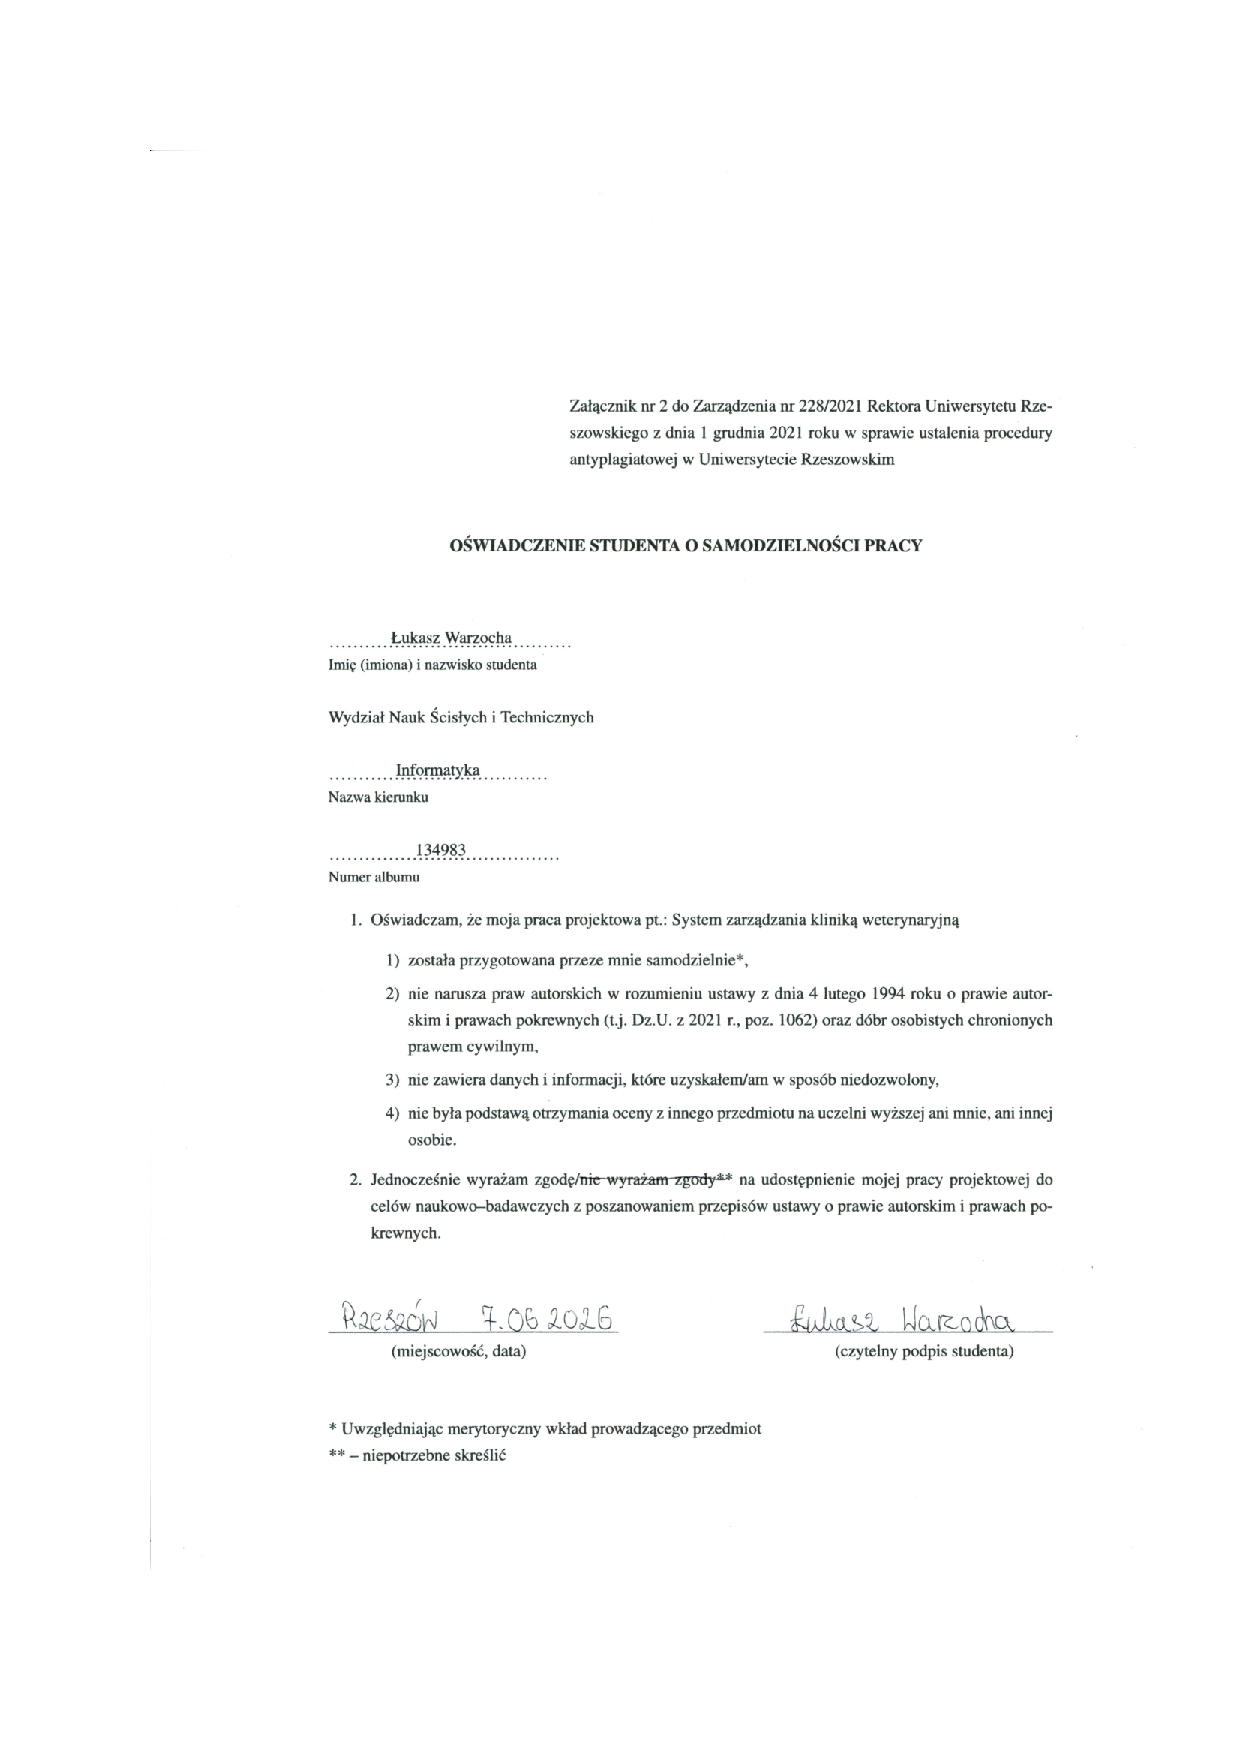
\includegraphics[width=\textwidth]{oswiadczenie.pdf}
\end{center}

\clearpage
\end{document}